\documentclass{article}
\usepackage{makeidx}
\usepackage{tabularx,colortbl}
\usepackage[dvipsnames]{xcolor}
\usepackage{flushend}
\usepackage{cite}
\usepackage{amsmath}
\usepackage{amssymb}
\usepackage{epsfig}
\usepackage{stmaryrd}
\usepackage{url}
\usepackage{amsmath}
\usepackage{bm}
\usepackage{amsthm}
\usepackage{amssymb}
\usepackage{multirow}
\usepackage{latexsym}
\usepackage{graphics}
\usepackage{graphicx}
\usepackage{enumitem}
\usepackage{comment}
\usepackage{longtable}
\usepackage{supertabular}
\usepackage{times}
\usepackage{listings}
\usepackage{subfigure}
\usepackage{color}
\usepackage{booktabs}
\usepackage{balance}
\usepackage{xspace}
\usepackage[ruled, vlined, linesnumbered]{algorithm2e}
\usepackage[autostyle]{csquotes}
\usepackage[]{algorithm2e}
\usepackage{authblk}
\newtheorem{theorem}{Theorem}
\newtheorem{definition}{Definition}
\newcommand{\mkeyword}[1]{\mbox{\texttt{#1}}}
\DeclareMathOperator{\kuop}{uop}
\DeclareMathOperator{\kbop}{bop}
\DeclareMathOperator{\kite}{ite}
\DeclareMathOperator{\kpre}{pre}
\DeclareMathOperator{\dom}{dom}
\DeclareMathOperator{\ktrue}{true}
\DeclareMathOperator{\kfalse}{false}
\DeclareMathOperator{\kselect}{select}
\DeclareMathOperator{\ran}{range}
\newcommand{\lbb}{[\![}
\newcommand{\rbb}{]\!]}
\newcommand{\expr}{\phi}
\newcommand{\exprS}{\Phi}
\newcommand{\mats}[1]{\textcolor{red}{#1}}
\newcommand{\janet}[1]{\textcolor{blue}{#1}}
\newcommand{\darren}[1]{\textcolor{green}{#1}}
\newcommand{\danielle}[1]{\textcolor{orange}{#1}}

\sloppypar
\widowpenalty10000



\begin{document}

\definecolor{gold}{rgb}{0.90,.66,0}
\definecolor{dgreen}{rgb}{0,0.6,0}
\newcommand{\stateequiv}{\equiv_{s}}
\newcommand{\traceequiv}{\equiv_{\sigma}}
\newcommand{\ta}{\text{TA}}
\newcommand{\cta}{\text{TA$_{C}$}}
\newcommand{\tta}{\text{TA$_{T}$}}
\newcommand{\ucalg}{\texttt{\small{IVC\_UC}}}
\newcommand{\ucbfalg}{\texttt{\small{IVC\_UCBF}}}


%
\title{Architectural Modeling and Analysis for Safety Engineering}
\author[1]{Danielle Stewart}
\author[2]{Jing (Janet) Liu}
\author[2]{Darren Cofer}
\author[1]{Mats Heimdahl}
\author[1]{Michael W. Whalen}
\author[3]{Michael Peterson}
\affil[1]{University of Minnesota Department of Computer Science and Engineering}
\affil[2]{Collins Aerospace: Trusted Systems - Enterprise Engineering}
\affil[3]{Collins Aerospace: Flight Controls Safety Engineering - Avionics}
\setcounter{Maxaffil}{0}
\renewcommand\Affilfont{\itshape\small}
\maketitle
\newpage
\tableofcontents
\newpage
\listoffigures
\listoftables
\listofalgorithms
\newpage

\begin{abstract}
%Mats' abstract
Model-based development tools are increasingly being used 
for system-level development of safety-critical systems. Architectural 
and behavioral models  provide important information 
that can be leveraged to improve the system
safety analysis process. Model-based design artifacts 
produced in early stage development activities can be used to perform system safety analysis,
reducing costs and providing accurate results throughout
the system life-cycle. In this report we describe an extension 
to the Architecture Analysis and Design Language (AADL) that 
supports modeling of system behavior under failure conditions. This 
\emph{Safety Annex} enables the independent modeling of component 
failures and allows safety engineers to weave various types of 
fault behavior into the nominal system model. The accompanying tool support 
uses model checking to propagate errors from their source to
 their effect on %top-level 
 safety properties without the need to add 
separate propagation specifications. %Our tools are also able to 
%compute minimal cut sets for the top level properties which are used to produce faults trees 
%familiar to safety engineers and certification authorities.  
The tool also captures all minimal set of fault combinations that can cause violation of the safety properties, that can be compared to qualitative and quantitative objectives as part of the safety assessment process.
We describe the Safety Annex, illustrate its use with a representative 
example, and discuss and demonstrate the tool support enabling an 
analyst to investigate the system behavior under failure conditions.	

\end{abstract}


\section{Introduction}
\label{sec:intro}

%This paper describes a new methodology with tool support for model based safety analysis. It is implemented as a {\em Safety Annex} for the Architecture Analysis and Design Language (AADL). The Safety Annex provides the ability to describe faults and faulty component behaviors in AADL models. In contrast to previous AADL-based approaches, the Safety Annex leverages a formal description of the nominal system behavior to propagate faults in the system. This approach ensures consistency with the rest of the system development process and simplifies the work of safety engineers. The language for describing faults is extensible and allows safety engineers to weave various types of faults into the nominal system model. The Safety Annex supports the injection of faults into component level outputs, and the resulting behavior of the system can be analyzed using model checking through the Assume-Guarantee Reasoning Environment (AGREE).

System safety analysis techniques are well-established and are a required activity in the development of safety-critical systems. Model-based systems engineering (MBSE) methods and tools based on formal methods now permit system-level requirements to be specified and analyzed early in the development process~\cite{NFM2012:CoGaMiWhLaLu,CAV2015:BoCiGrMa}. While model-based development methods are widely used in the aerospace industry, they are only recently being applied to system safety analysis.  

%How can we leverage these model-based methods and tools to perform safety analysis based on models of the system architecture and initial functional decomposition? Can these design models be integrated into the safety analysis process to help guarantee accurate and consistent results?
%Seeking solutions to these questions are especially important as the amount of safety-critical hardware and software in various domains has drastically increased due to the demand for greater autonomy, capability, and connectedness.

In this paper, we describe a {\em Safety Annex} for the Architecture Analysis and Design Language (AADL)~\cite{FeilerModelBasedEngineering2012} that provides the ability to reason about faults and faulty component behaviors in AADL models. In the Safety Annex approach, we use formal assume-guarantee contracts to define the nominal behavior of system components. The nominal model is then verified using the Assume Guarantee Reasoning Environment (AGREE)~\cite{NFM2012:CoGaMiWhLaLu}. The Safety Annex  provides a way to weave faults into the nominal system model and analyze the behavior of the system in the presence of faults. The Safety Annex also provides a library of common fault node definitions that is customizable to the needs of system and safety engineers. Our approach adapts the work of Joshi et. al in
~\cite{Joshi05:Dasc} to the AADL modeling language, and provides a domain specific language for the kinds of analysis performed manually in previous work~\cite{Stewart17:IMBSA}.  %More information on the approach is available in~\cite{Stewart17:IMBSA}, and the tool and relevant documentation can be found at: \small \url{https://github.com/loonwerks/AMASE/}. \normalsize

There are other tools purpose-built for safety analysis, including AltaRica~\cite{PROSVIRNOVA2013127}, smartIFlow~\cite{info8010007} and xSAP~\cite{DBLP:conf/tacas/BittnerBCCGGMMZ16}. These notations are separate from the system development model. Other tools extend existing system models, such as HiP-HOPS~\cite{CHEN201391} and the AADL Error Model Annex, Version 2 (EMV2)~\cite{EMV2}. EMV2 uses enumeration of faults in each component and explicit propagation of faulty behavior to perform safety analysis. The required propagation relationships must be manually added to the system model and can become complex, leading to potential omissions and inconsistencies.

In contrast, the Safety Annex supports model checking and quantitative reasoning by attaching behavioral faults to components and then using the normal behavioral propagation and proof mechanisms built into the AGREE AADL annex. This allows users to reason about the evolution of faults over time, and produce counterexamples demonstrating how component faults lead to system failures. It can serve as the shared model to capture system design and safety-relevant information, and produce both qualitative and quantitative description of the causal relationship between faults/failures and system safety requirements.
%
Thus, the contributions of the Safety Annex and this paper are:
\begin{itemize}
\item Close integration of behavioral fault analysis into an {\em architectural design language} AADL, which allows close connection between system and safety analysis and system generation from the model (unlike AltaRica, smartIFlow, and xSAP),
\item support for {\em behavioral specification of faults} and their {\em implicit propagation} through behavioral relationships in the model, in contrast to existing AADL-based annexes (HiP-HOPS and EMV2),
\item additional support for {\em explicit} propagation of faults to capture binding relationships between hardware and software and logical and physical communications beyond what is supported in xSAP, and
\item guidance on integration into a traditional safety analysis process.
\end{itemize}
%\mike{What are our contributions?}


\section{Preliminaries}
\label{sec:prelims}
One of our goals is to transition the tools we have developed into use by the safety engineers who perform safety assessment of avionics products. Therefore, we need to understand how the tools and the models will fit into the existing safety assessment and certification process.
\subsection{Safety Assessment Process}
\label{subsec:process}

%ARP4754A, the Guidelines for Development of Civil Aircraft and Systems~\cite{SAE:ARP4754A}, has been recognized by the Federal Aviation Administration (FAA) as 
%an ``acceptable method for establishing a development assurance process''~\cite{AC:20-174}. It provides guidance on applying development assurance at each hierarchical level throughout the development life cycle of highly-integrated/complex aircraft systems.

ARP4754A, the Guidelines for Development of Civil Aircraft and Systems~\cite{SAE:ARP4754A}, provides guidance on applying development assurance at each hierarchical level throughout the development life cycle of highly-integrated/complex aircraft systems, and has been recognized by the Federal Aviation Administration (FAA) as an acceptable method to establish the assurance process.

%Figure~\ref{fig:arp4754a_process} from [ref. ARP4754A] demonstrates the ARP4754A process flow.

The safety assessment process is a starting point at each hierarchical level of the development life cycle, and is tightly coupled with the system development and verification processes. It is used to show compliance with certification requirements, and for meeting a company's internal safety standards. ARP4761, the Guidelines and Methods for Conducting Safety Assessment Process on Civil Airborne Systems and Equipment~\cite{SAE:ARP4761},  identifies a systematic means to show compliance. The guidelines presented in ARP4761 include industry accepted safety assessment processes (Functional Hazard Assessment (FHA), Preliminary System Safety Assessment (PSSA), and System Safety Assessment (SSA)), and safety analysis methods to conduct the safety assessment, 
such as Fault Tree Analysis (FTA), Failure Modes and Effect Analysis (FMEA), and Common Cause Analysis (CCA).

A prerequisite of performing the safety assessment of a system design is to understand how the system is intended to work, primarily focusing on the integrity of the outputs and the availability of the system. The safety engineers then use the acquired understanding to conduct safety analysis, construct the safety analysis artifacts, and compare the analysis results with established safety objectives and safety-related requirements. 

%In practice, prior to performing the safety assessment of a system, the safety engineers are often equipped with the domain knowledge about the system, but do not necessarily have detailed knowledge of the current system is implemented. Acquiring the required knowledge about the behavior and implementation of each software function in a system can be time-consuming. 

In practice, prior to performing the safety assessment of a system, the safety engineers are often equipped with the domain knowledge about the system, but do not necessarily have detailed knowledge of how the software functions are designed. Acquiring the required knowledge about the behavior and implementation of each software function in a system can be time-consuming.

For example, in a recent project it took one of our safety engineers two days to understand how the software in a Stall Warning System was intended to work. The primary task includes connecting the signal and function flows to relate the input and output signals from end-to-end and understanding the causal effect between them. This is at least as much time as was required to construct the safety analysis artifacts and perform the safety analysis itself. In another instance, it took a safety engineer several months to finalize the PSSA document for a Horizontal Stabilizer Control System, because of two major design revisions requiring multiple rounds of reviews with system, hardware, and software engineers to establish complete understanding of the design %implementation 
details.

Industry practitioners have come to realize the benefits and importance of
using models to assist the safety assessment process (either by augmenting the existing system design model, or by building a separate safety model), and a revision of the ARP4761 to include {\em model based safety analysis} is under way.
Capturing failure modes in models and generating safety analysis artifacts directly from models could greatly improve communication and synchronization between system designer and safety engineers, and provide the ability to more accurately analyze complex systems. 

We believe that using a single unified model to conduct both system development and safety analysis can help reduce the gap in comprehending the system behavior and transferring the knowledge between the system designers and the safety analysts. It maintains a living model that captures the current state of the system design as it moves through the system development lifecycle.
%Figure~\ref{fig:arp4754a_process}.
It also allows all participants of the ARP4754A process to be able to communicate and review the system design using a ``single source of truth.''

A model that supports both system design and safety analysis must describe both the system design information (e.g., system architecture, functional behavior) and safety-relevant information (e.g., failure modes, failure rates).  It must do this in a way that keeps the two types of information distinguishable, yet allows them to interact with each other.

\begin{figure}[t!]
	\vspace{-0.19in}
	\centering
	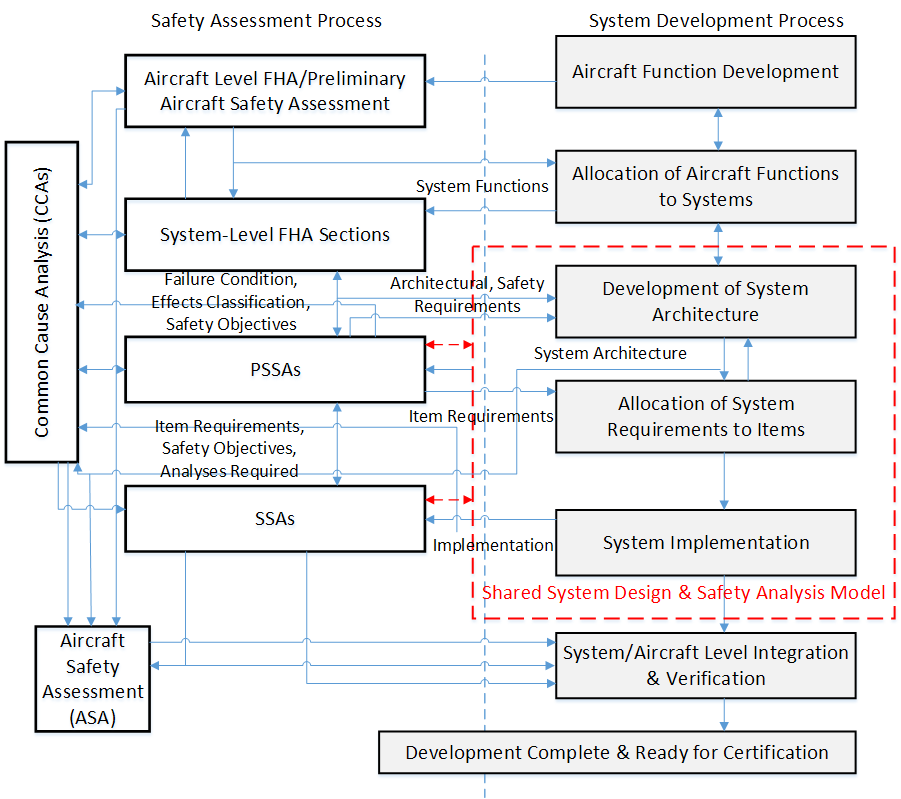
\includegraphics[trim=0 9 0 5,clip,width=0.85\textwidth]{images/Safety_Assessment_Process.png}
	%\vspace{0.4in}
	\caption{Using the Shared System/Safety Model in the ARP4754A Safety Assessment Process}
	\label{fig:proposed_safety_process}
\end{figure}

Figure~\ref{fig:proposed_safety_process} presents our proposed use of this shared system design and safety analysis model in the context of the ARP4754A Safety Assessment Process Model (derived from Figure 7 of ARP4754A). The shared model is one of the system development artifacts from the ``Development of System Architecture'' and ``Allocation of System Requirements to Item'' activities in the System Development Process, which interacts with the PSSAs and SSAs activities in the Safety Assessment Process. The shared model can serve as an interface to capture the information from the system design and implementation that is relevant for the safety analysis.

\begin{figure}[t!]
	\vspace{-0.19in}
	\centering
	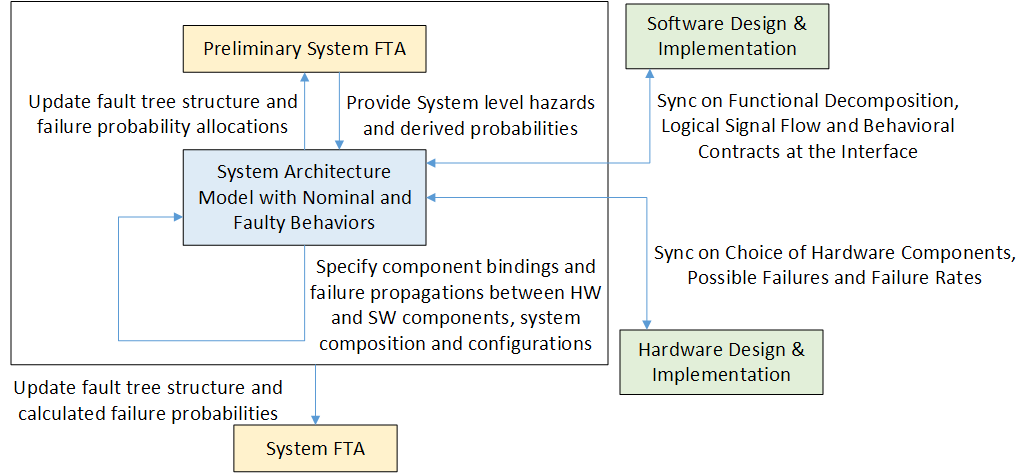
\includegraphics[width=0.9\textwidth]{images/FTA_MBD_Workflow.png}
	%\vspace{-0.19in}
	\caption{Example Interactions between the Shared System/Safety Model and the FTAs}
	\label{fig:interaction_with_FTA}
\end{figure}

Figure~\ref{fig:interaction_with_FTA} shows how the preliminary FTAs and final system FTAs (artifacts from the PSSA and SSA activities in the Safety Assessment Process) can guide and be updated from the shared model.
%\darren{Maybe we need a couple of sentences to explain what's happening in the figure.}
The shared model is expected to be created and maintained in sync with the software and hardware design and implementation, and guided by the hazard and probability information from the preliminary system FTA. The analysis results from checking the system level properties on the shared model are then used to update the preliminary system FTA. This process continues iteratively until the system safety property is satisfied with the desired fault tolerance and failure probability achieved. The effort needed to update the final system FTA from the preliminary system FTA would be greatly reduced.




\subsection{Modeling Language for System Design}
\label{subsec:aadl-agree}
Figure~\ref{fig:proposed_safety_process} presents our proposed use of a single unified model to support both system design and safety analysis. It describes both system design and safety-relevant information 
that are kept distinguishable and yet are able to interact with each other. The shared model is a living model that captures the current state of the system design as it moves through the development lifecycle, allowing all participants of the \gls{arp}4754A process to be able to communicate and review the system design. Safety related information can be generated directly through automated analysis on the model. This provides the capability to more accurately analyze complex systems. The generated safety information includes counterexamples which show causal failure scenarios and minimal sets of fault combinations that cause the failure condition to occur.

\begin{figure}[t!]
	
	\centering
	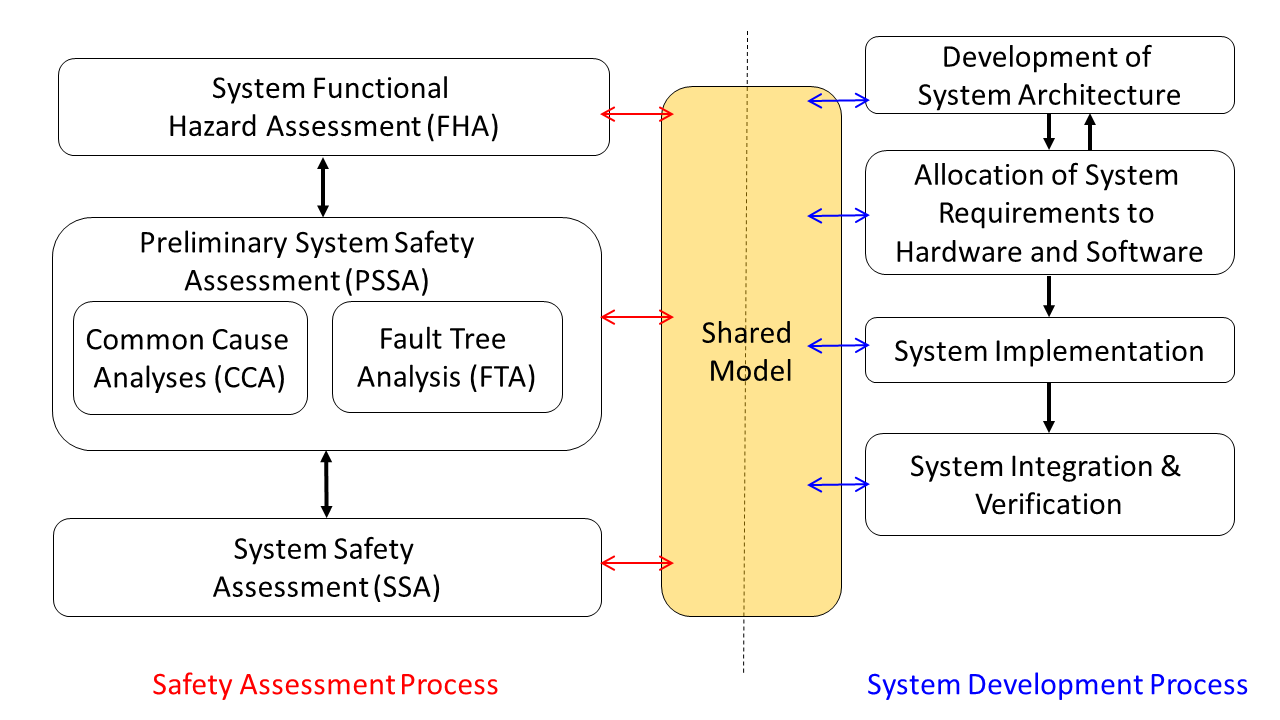
\includegraphics[trim=0 5 0 5,clip,width=0.85\textwidth]{images/process3.png}
	
	\caption{Use of the Shared System/Safety Model in the ARP4754A Safety Assessment Process}
	\label{fig:proposed_safety_process}
\end{figure}

We are using the Architectural Analysis and Design Language (AADL)~\cite{FeilerModelBasedEngineering2012} to construct system architecture models.  \gls{aadl} is an SAE International standard that defines a language and provides a unifying framework for describing the system architecture for ``performance-critical, embedded, real-time systems''~\cite{AADL_Standard}. From its conception, \gls{aadl} has been applied to the design and construction of avionics systems.  
Rather than being merely descriptive, \gls{aadl} models can be made specific enough to support system-level code generation.  Thus, results from analyses conducted, including the new safety analysis proposed here, correspond to the system that will be built from the model.  

An \gls{aadl} model describes a system in terms of a hierarchy of components and their interconnections, where each component can either represent a logical entity (e.g., application software functions, data) or a physical entity (e.g., buses, processors, memory). An \gls{aadl} model can be extended with language annexes to provide a richer set of modeling elements for various system design and analysis needs (e.g., performance-related characteristics, configuration settings, dynamic behaviors). The language definition is sufficiently rigorous to support formal analysis tools that allow for early phase error/fault detection.

The \gls{agree}~\cite{NFM2012:CoGaMiWhLaLu} is a tool for formal analysis of behaviors in \gls{aadl} models.  \gls{agree} is implemented as an \gls{aadl} annex and annotates \gls{aadl} components with formal behavioral contracts. Each component's contracts can include assumptions and guarantees about the component's inputs and outputs respectively, as well as predicates describing how the state of the component evolves over time. \gls{agree} translates an \gls{aadl} model and the behavioral contracts into Lustre~\cite{Halbwachs91:IEEE} and then queries the JKind
model checker~\cite{2017arXiv171201222G} to conduct the back-end analysis. The analysis %is
can be performed compositionally following the architecture hierarchy such that analysis at a higher level is based on the components at the next lower level.  When compared to monolithic analysis (i.e., analysis of the flattened model composed of all components), the compositional approach allows the analysis to scale to much larger systems~\cite{NFM2012:CoGaMiWhLaLu}. 

%In the avionics context, the software functions/applications, the hardware equipment, and the system that is composed of their integration can all be represented as components connected to/composed of/bind to other components in a hierarchical AADL model. AGREE contracts can be used to capture the functional requirements at each level of the hierarchy. Once the model has been reviewed and the requirements captured have been validated, the back-end analysis can be conducted to verify if each level of the model implements its higher level requirements correctly.

%AADL with the AGREE extension serves as a good candidate as the modeling language for describing the system design aspects of a shared system design and safety analysis model. 
%In our prior work~\cite{Stewart17:IMBSA}, we added an initial failure effect modeling capability to the AADL/AGREE language and tool set.  We are continuing this work so that our tools and methodology can be used to satisfy system safety objectives of ARP4754A and ARP4761.  

\begin{comment}
In particular, our goals are to:

\begin{itemize}
	\item Provide a comprehensive, qualitative description of the causal relationship between basic failure events and system level safety requirements.
	\item Provide an accurate, quantitative description of the contribution relationship between failure rates of the fault tree basic events and numerical probability requirements at the system level.
\end{itemize}
\end{comment}
%The remainder of the paper describes our approach towards both of the goals.





\subsection{Model-Based Safety Assessment Process Supported by Formal Methods}
\label{subsec:process}
We propose a model-based safety assessment process backed by formal methods to help safety engineers with early detection of the design issues.  This process uses a single unified model to support both system design and safety analysis. It is based on the following steps:

\begin{enumerate}
	\item System engineers capture the critical information in a shared AADL/AGREE model:  high-level hardware and software architecture, nominal behavior at the component level, and safety requirements at the system level.% (e.g., inhibit throttle movement during critical takeoff phase).
	\item System engineers use the backend model checker to verify that the safety requirements are satisfied by the nominal design model. 
	\item Safety engineers use the Safety Annex to augment the nominal model with the component failure modes. % (e.g., processor failure, input signal corrupted).  
	In addition, safety engineers specify the fault hypothesis for the analysis which corresponds to how many simultaneous faults the system must be able to tolerate.
	\item Safety engineers use the backend model checker to analyze if the safety requirements and fault tolerance objectives are satisfied by the design in the presence of faults. % (e.g., if the system is resilient to a single failure). 
	If the design does not tolerate the specified number of faults (or probability threshold of fault occurrence), then the tool produces counterexamples leading to safety requirement violation in the presence of faults, %and also
	 as well as all minimal set of fault combinations that can cause the safety requirement to be violated.
	%produces fault trees showing smallest set of faults that may lead to the safety requirement being violated. 
	\item The safety engineers examine the results to assess the validity of the fault combinations and the fault tolerance level of the system design. If a design change is warranted, the model will be updated with the latest design change and the above process is repeated.
\end{enumerate}

There are other tools purpose-built for safety analysis, including AltaRica~\cite{PROSVIRNOVA2013127}, smartIFlow~\cite{info8010007} and xSAP~\cite{DBLP:conf/tacas/BittnerBCCGGMMZ16}. These tools and their accompanying notations are separate from the system development model. Other tools extend existing system models, such as HiP-HOPS~\cite{CHEN201391} and the AADL Error Model Annex, Version 2 (EMV2)~\cite{EMV2}. EMV2 uses enumeration of faults in each component and explicit propagation of faulty behavior to perform error analysis. The required propagation relationships must be manually added to the system model and can become complex and lead to mistakes in the analysis.

In contrast, the Safety Annex supports model checking and quantitative reasoning by attaching behavioral faults to components and then using the normal behavioral propagation and proof mechanisms built into the AGREE AADL annex.  This allows users to reason about the evolution of faults over time, and produce counterexamples demonstrating how component faults lead to failures.
Our approach adapts the work of Joshi et. al
~\cite{Joshi05:Dasc} to the AADL modeling language.  Stewart, et. al provide more information on the approach~\cite{Stewart17:IMBSA}, and the tool and relevant documentation can be found at: \small \url{https://github.com/loonwerks/AMASE/}. \normalsize

%\subsection{Comparison with EMV2}
\label{subsec:comparison_with_EMV2}

The AADL language has previously been extended to provide some fault modeling and analysis capabilities using its Error Model Annex, Version 2 (EMV2)~\cite{EMV2}.  EMV2 focuses on injection and propagation of discrete faults for generation of fault trees, rather than on analysis of system behavior in the presence of faults. In order for a component to have an impact on the rest of the system, all faults must be explicitly propagated through each component by applying fault types on each of the output ports. When using this type of fault analysis, the safety analyst must understand the system  behavior and component functions well enough to specify how a failure will propogate through the system, what the destination components reaction to said failure will be, and correctly implement these propagations. In EMV2, every possible component failure must be specified in this way. As a contrast, the Safety Annex provides two ways in which to specify these faults. The explicit propagation capability in the Safety Annex is meant to capture hardware faults and faults that occur due to colocated components. In every other instance, implicit propagation is used through the behavior model. In related work, comparisons with other related toolsets is explored in more depth. 














\iffalse

The AADL language has previously been extended to provide some fault modeling and analysis capabilities using its Error Model Annex, Version 2 (EMV2)~\cite{EMV2}.  EMV2 focuses on injection and propagation of discrete faults for generation of fault trees, rather than on analysis of system behavior in the presence of faults. 
To illustrate some of the key differences between our approach and the EMV2 approach, Figure~\ref{fig:comparison_with_EMV2} shows a simplified example based on an aircraft Wheel Brake System (WBS). The WBS model is described in greater detail in ~\cite{Stewart17:IMBSA} and in Section \ref{sec:case_study}. The code fragments in the figure extracted from EMV2, AGREE, and the Safety Annex do not represent the complete code.

\begin{figure}[t]
	\vspace{-0.19in}
	\centering
	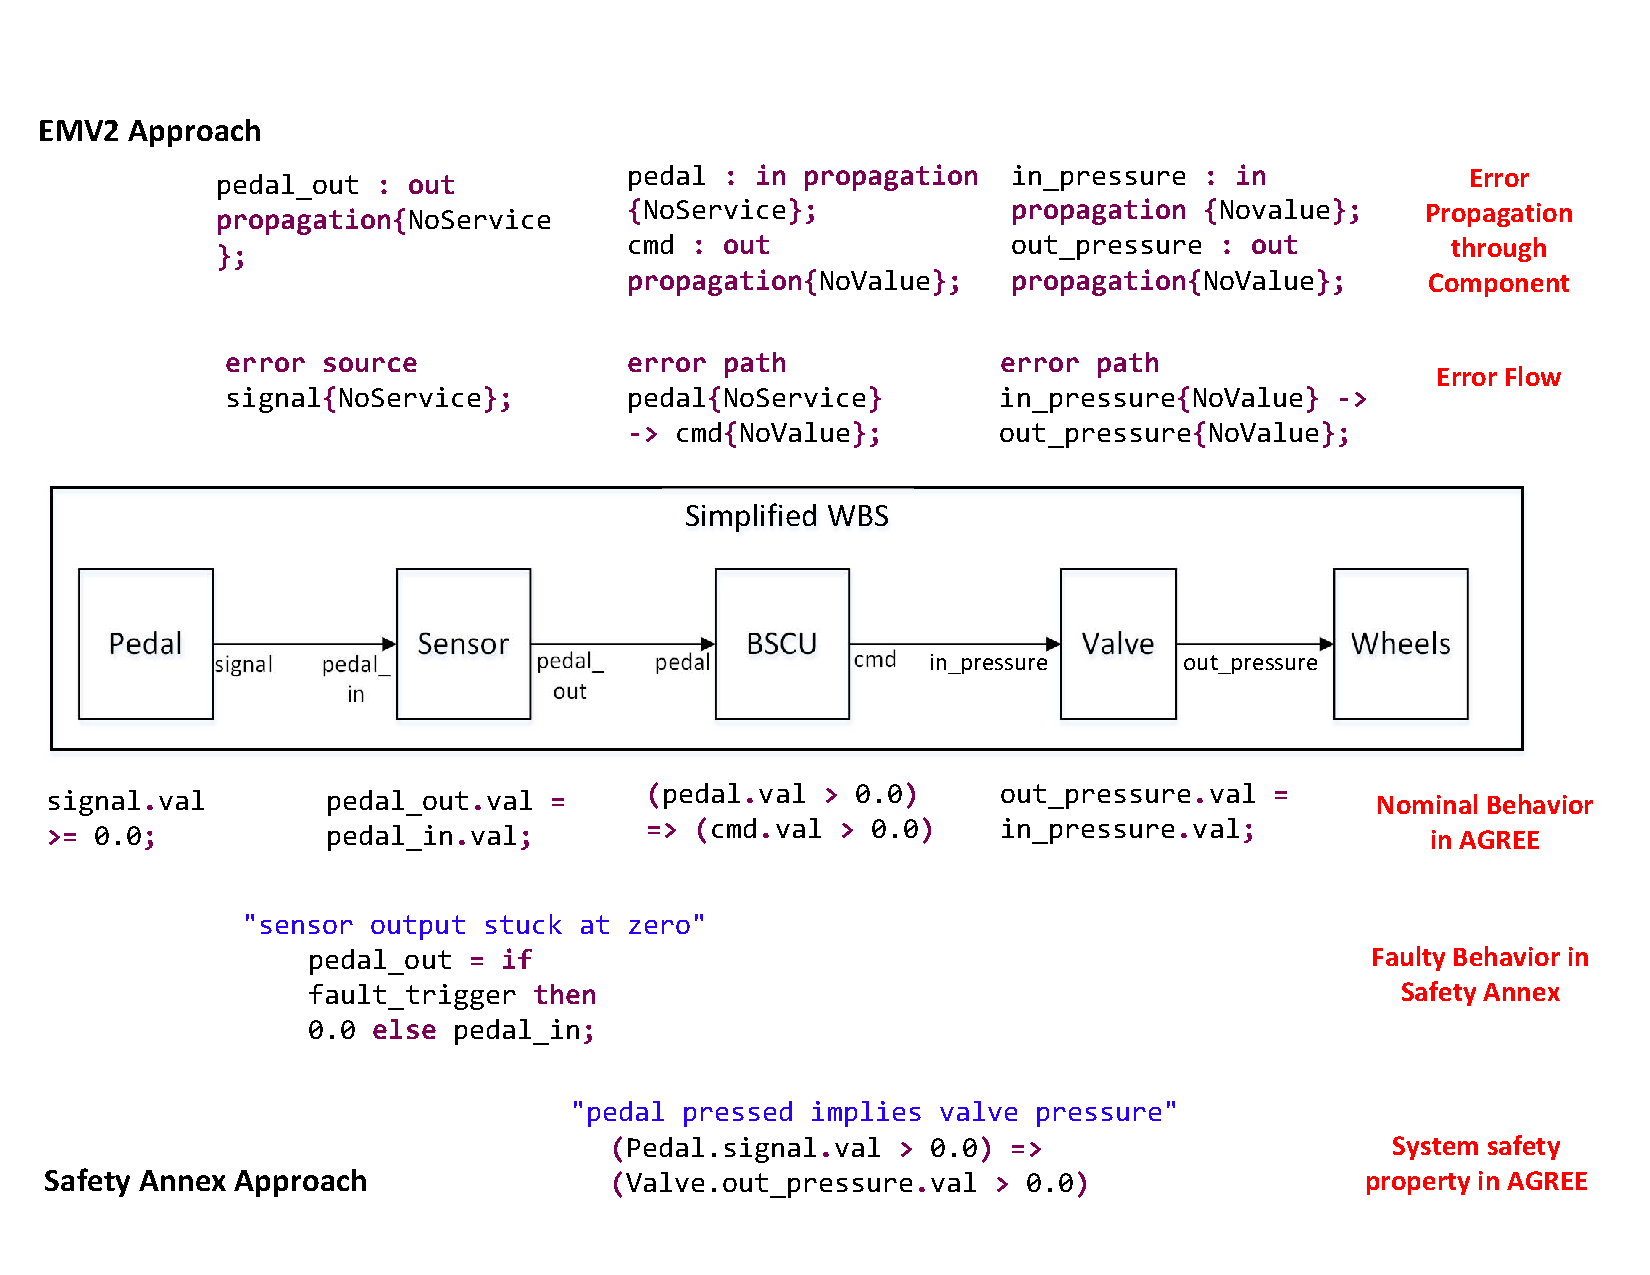
\includegraphics[trim=0 9 0 5,clip,width=\textwidth]{images/Comparison_with_EMV2.pdf}
	%\vspace{0.4in}
	\caption{Differences between Safety Annex and EMV2}
	\label{fig:comparison_with_EMV2}
\end{figure} 

In our simplified WBS system, the physical signal from the Pedal component in detected by the Sensor, and the pedal position value is passed to the Braking System Control Unit (BSCU) components.  The BSCU generates a pressure command to the Valve component which applies hydraulic brake pressure to the Wheels. In this example, we use the general term ``fault'' to denote all component errors, hardware failures, and system faults captured by both approaches.

In the EMV2 approach (top half of Figure~\ref{fig:comparison_with_EMV2}), all faults must be explicitly propagated through each component (by applying fault types on each of the output ports) in order for a component to have an impact on the rest of the system. In the example, the ``NoService'' fault is explicitly allowed by the EMV2 declarations to propagate through all of the components.  These fault types are essentially tokens that do not capture any analyzable behavior.  At the system level, analysis tools supporting the EMV2 annex can aggregate the fault flow and propagation information from different components to compose an overall fault flow diagram or fault tree.

In the Safety Annex approach (bottom half of Figure~\ref{fig:comparison_with_EMV2}), faults are captured as faulty behaviors that augment the system behavioral model in AGREE contracts.  When a fault is triggered, the output behavior of the Sensor component is modified, in this case resulting a ``stuck at zero'' error. The behavior of the BSCU receives a zero input and proceeds as if the pedal has not been pressed. This will cause the top level system contract to fail: {\em pedal pressed implies brake pressure output is positive}. No explicit fault propagation is necessary since the faulty behavior itself propagates through the system just as in the nominal system model. The effects of any triggered fault are manifested through analysis of the AGREE contracts. 


 \fi





\subsection{Comparison with Proposed MBSA Appendix to ARP4761A}
\label{sec:mbsa_appendix_review}

ARP4754A, the Guidelines for Development of Civil Aircraft and Systems~\cite{SAE:ARP4754A}, provides guidance on applying development assurance at each hierarchical level throughout the development life cycle of highly-integrated/complex aircraft systems. ARP4761, the Guidelines and Methods for Conducting Safety Assessment Process on Civil Airborne Systems and Equipment~\cite{SAE:ARP4761},  identifies a systematic means to show compliance. A Model Based Safety Analysis (MBSA) appendix has been drafted to the upcoming revision of ARP4761 to provide concepts and processes with Model Based Safety Analysis.

We have reviewed the draft appendix and found that our approach is consistent with the MBSA appendix in the following ways:

\begin{itemize}
	\item The common goal is to use MBSA for an equivalent analysis to the traditional safety analysis methods (e.g., Fault Trees) to support safety assessment processes.
	\item Both use an analytical model of the system to capture failure propagation. In the model, system architecture, nominal and faulty functional behaviors are captured. The model evolves as the system design evolves.
	\item Both use software application/tools to perform analysis on the model and generate outputs (e.g., failure sequences, minimal cut sets that result in the failure condition under analysis). The MBSA appendix also mentioned that model checking can be used to perform an exhaustive exploration of the state space of the model.
	\item Outputs generated from the analysis are to be compared to qualitative and/or quantitative objectives and requirements as part of the safety assessment process. Furthermore, the outputs drive evolution of system design. 
\end{itemize}

Our approach goes beyond what is envisioned in the MBSA appendix in the following ways:

\begin{itemize}
	\item The MBSA Appendix is not advocating a single unified model used by both system development and safety assessment activities. The model is safety specific and driven by the types of safety assessment to be conducted. However, the initial safety model may be derived from the system design model, and may be closer to the design at the lower levels of the design process.
	\item In the MBSA Appendix, the failure propagation modeling focuses on the inside internal flows in the components, which is similar to the bottom-up method in Failure Modes and Effects Analysis. Different components are connected by inputs and outputs, and no behavioral constraints are specified on data entering and exiting components. This leaves inter-component propagation to be explored by the analysis.
\end{itemize}

In summary, our approach provides a new way to do safety analysis. It uses an unified model that is shared by system development and safety assessment. The model captures architecture and behavioral information for propagation within components and between components. It is a property driven approach that is consistent between system verification and safety analysis.










































\section{Fault Modeling with the Safety Annex}
\label{sec:fault_modeling}

To demonstrate the fault modeling capabilities of the Safety Annex we will use the Wheel Brake System (WBS) described in AIR6110~\cite{AIR6110}.  This system is a well-known example that has been used as a case study for safety analysis, formal verification, and contract based design~\cite{DBLP:conf/cav/BozzanoCPJKPRT15, 10.1007/978-3-319-11936-6-7, CAV2015:BoCiGrMa, Joshi05:SafeComp}. The preliminary work for the safety annex was based on a simple model of the WBS~\cite{Stewart17:IMBSA}. To demonstrate a more complex fault modeling process, we constructed a functionally and structurally equivalent AADL version of the more complex WBS NuSMV/xSAP models~\cite{DBLP:conf/cav/BozzanoCPJKPRT15}.    

\begin{figure}[h!]
	\centering
	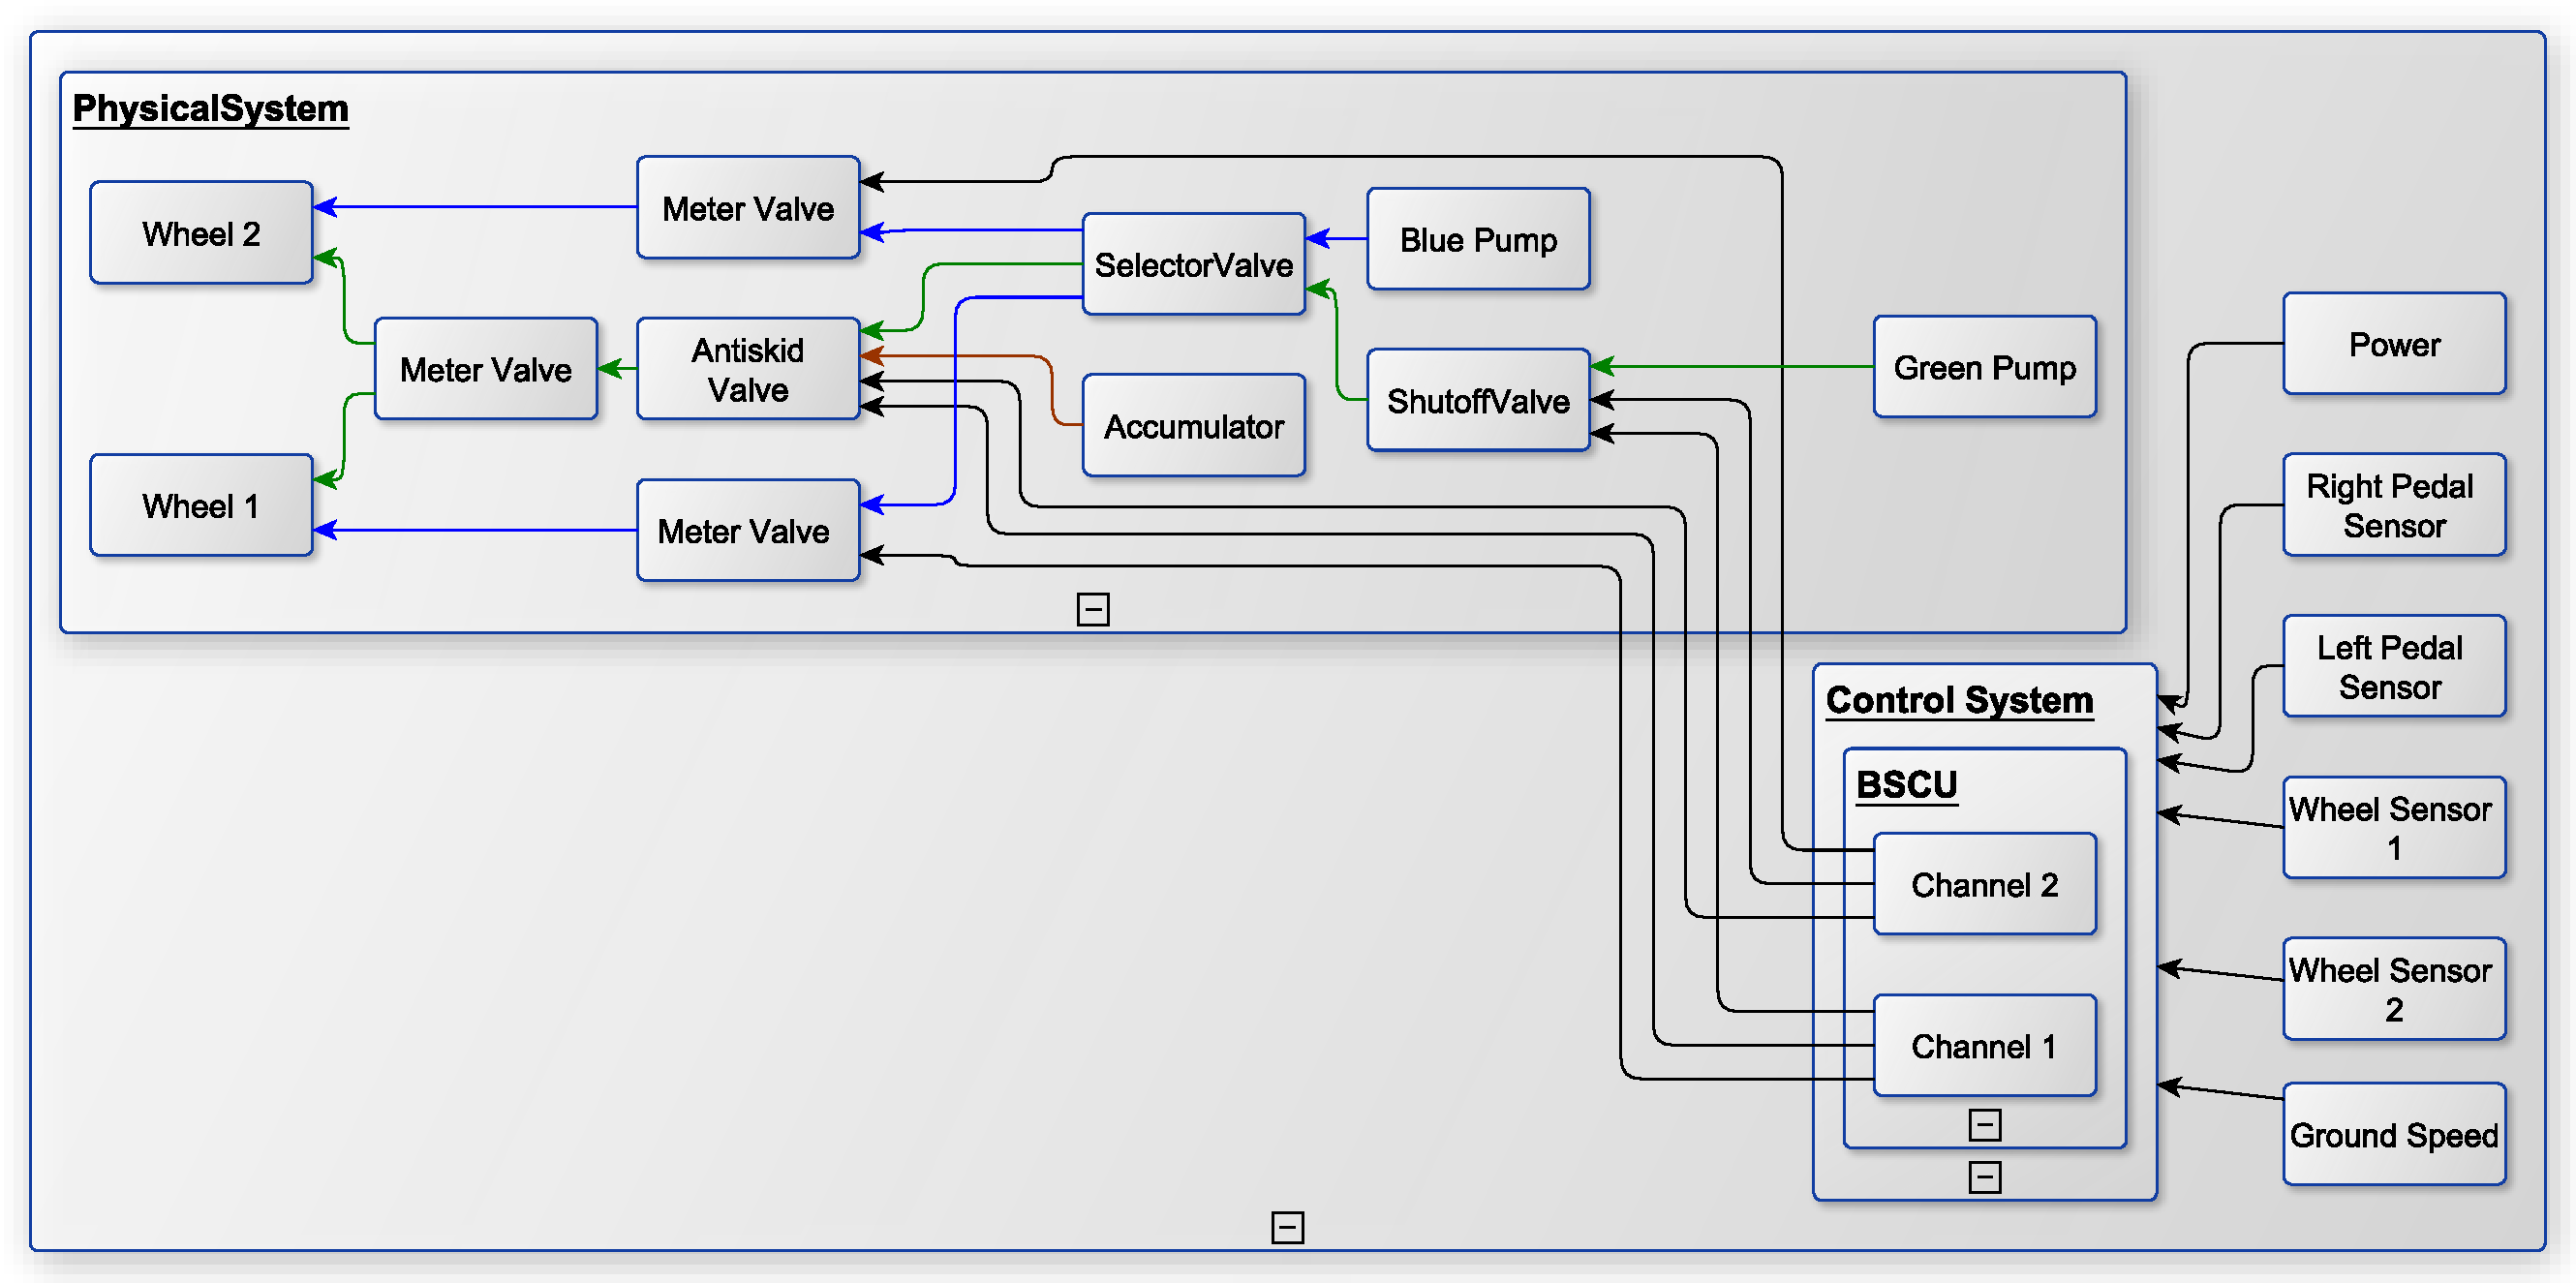
\includegraphics[trim=0 9 0 5,clip,width=\textwidth]{images/wbs_arch4_diagram.pdf}
	\caption{Wheel Brake System}
	\label{fig:wbs}
\end{figure} 

The WBS is composed of two main parts: the Line Replaceable Unit control system and the electro-mechanical physical system.
The control system electronically controls the physical system and contains a redundant
channel of the Braking System Control Unit (BSCU) in case a detectable fault occurs in the active channel.
 It also commands antiskid braking. % in case of skidding on the ground. 
 The physical system consists of the hydraulic circuits running from hydraulic pumps to wheel brakes as well as valves that control the hydraulic fluid flow. This system provides braking force to each of the eight wheels of the aircraft. The wheels are all mechanically braked in pairs (one pair per landing gear). For simplicity, Figure~\ref{fig:wbs} displays only two of the eight wheels. 

There are three operating modes in the WBS model:

\begin{itemize}
	\renewcommand{\labelitemi}{\textbullet}
	\item In \textit{normal} mode, the system is composed of a \textit{green} hydraulic pump and one meter valve per each of the eight wheels. Each of the meter valves are controlled through electronic commands coming from the active channel of the BSCU. These signals provide braking and antiskid commands for each wheel. The braking command is determined through a sensor on the pedal and the antiskid command is determined by the \textit{Wheel Sensors}. 
	\item In \textit{alternate} mode, the system is composed of a \textit{blue} hydraulic pump, four meter valves, and four antiskid shutoff valves, one for each landing gear. The meter valves are mechanically commanded through the pilot pedal corresponding to each landing gear. If the selector detects lack of pressure in the green circuit, it switches to the blue circuit. 
	\item In \textit{emergency} mode, the system mode is entered if the \textit{blue} hydraulic pump fails. The accumulator pump has a reserve of pressurized hydraulic fluid and will supply this to the blue circuit in emergency mode. 
\end{itemize}

The WBS architecture model in AADL contains 30 different kinds of components, 169 component instances, and a model depth of 5 hierarchical levels. 


%If the BSCU channel becomes invalid, the shutoff valve closes and we move into alternate mode. Once this system switches into alternate mode, it does not return to normal operation mode.

%There are three operating modes in the WBS model. In \textit{normal} mode, the system uses the \textit{green} hydraulic circuit. The normal system is composed of the green hydraulic pump and one meter valve per each of the eight wheels. Each of the meter valves are controlled through electronic commands coming from the active channel of the BSCU. These signals provide braking and antiskid commands for each wheel. The braking command is determined through a sensor on the pilot pedal position and is labeled as \textit{Left/Right Pedal Sensor} in Figure~\ref{fig:wbs} and the antiskid command is determined by the \textit{Wheel Sensors}. 

%In \textit{alternate} mode, the system uses the \textit{blue} hydraulic circuit. The alternate system is composed of the blue hydraulic pump, four meter valves, and four antiskid shutoff valves: one for each landing gear. The meter valves are mechanically commanded through the pilot pedal corresponding to each landing gear. If the system detects lack of pressure in the green circuit, the BSCU channel commands the selector valve to switch to the blue circuit. 
%If the BSCU channel becomes invalid, the shutoff valve closes and we move into alternate mode. Once this system switches into alternate mode, it does not return to normal operation mode.

%The last mode of operation of the WBS is the \textit{emergency} mode. This mode is entered if the blue hydraulic pump fails. The accumulator pump has a reserve of pressurized hydraulic fluid and will supply this to the blue circuit in emergency mode.

%The model contains 30 different kinds of components, 169 component instances, a model depth of 5 hierarchical levels.  The model includes one top-level assumption and  11 top-level system properties, with 113 guarantees allocated to subsystems.  There are a total of 33 different fault types and 141 fault instances within the model.  The large number of fault instances is due to the redundancy in the system design and its replication to control 8 wheels.

The behavioral model is encoded using the AGREE annex and the behavior is based on descriptions found in AIR6110. The top level system properties are given by the requirements and safety objectives in AIR6110. All of the subcomponent contracts support these system safety objectives through the use of assumptions on component input and guarantees on the output. The WBS behavioral model in AGREE annex includes one top-level assumption and  11 top-level system properties, with 113 guarantees allocated to subsystems.  

An example system safety property is to ensure that there is no inadvertent braking of any of the wheels. This is based on a failure condition described in AIR6110 is \textit{Inadvertent wheel braking on one wheel during takeoff shall be less than 1E-9 per takeoff}. 
Inadvertent braking means that braking force is applied at the wheel but the pilot has not pressed the brake pedal.  In addition, the inadvertent braking requires that power and hydraulic pressure are both present, the plane is not stopped, and the wheel is rolling (not skidding). The property is stated in AGREE such that inadvertent braking does \textit{not} occur, as shown in Figure \ref{fig:inadvertent_braking}. 

\begin{figure}[h!]
	%\vspace{-0.2in}
	\begin{center}
		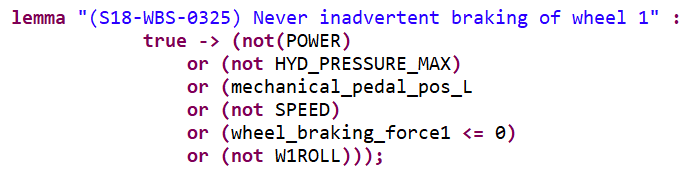
\includegraphics[width=.7\textwidth]{images/inadvertent_braking.png}
	\end{center}
	\vspace{-0.3in}
	\caption{AGREE Contract for Top Level Property: Inadvertent Braking}
	\label{fig:inadvertent_braking}
	%\vspace{-0.2in}
\end{figure}


\subsection{Component Fault Modeling}

The usage of the terms error, failure, and fault are defined in ARP4754A and are described here for ease of understanding~\cite{SAE:ARP4754A}. An \textit{error} is a mistake made in implementation, design, or requirements. A \textit{fault} is the manifestation of an error and a \textit{failure} is an event that occurs when the delivered service of a system deviates from correct behavior. If a fault is activated under the right circumstances, that fault can lead to a failure. The terminology used in EMV2 differs slightly for an error: an error is a corrupted state caused by a fault. The error propagates through a system and can  manifest as a failure. In this report, we use the ARP4754A terminology with the added definition of \textit{error propagation} as used in EMV2. An error is a mistake made in design or code and an error propagation is the propagation of the corrupted state caused by an active fault. 

The Safety Annex is used to add possible faulty behaviors to a component model. Within the AADL component instance model, an annex is added which contain the fault definitions for the given component. The flexibility of the fault definitions allows the user to define numerous types of fault \textit{nodes} by utilizing the AGREE node syntax. A library of common fault nodes has been written and is available in the project GitHub repository~\cite{SAGithub}. Examples of such faults include valves being stuck open or closed, output of a software component being nondeterministic, or power being cut off.  When the fault analysis requires fault definitions that are more complex, these nodes can easily be written and used in the model. 

When a fault is activated by its specified triggering conditions, it modifies the output of the component. This faulty behavior may violate the contracts of other components in the system, including assumptions of downstream components. The impact of a fault is computed by the AGREE model checker when the safety analysis is run on the fault model. 

The majority of faults that are connected to outputs of components are known as \textit{symmetric}. That is, whatever components receive this faulty output will receive the same faulty output value. Thus, this output is seen symmetrically. An alternative fault type is \textit{asymmetric}. This pertains to a component with a 1-n output: one output which is sent to many receiving components. This fault can present itself differently to the receiving components. For instance, in a boolean setting, one component might see a true value and the rest may see false. This is also possible to model using the keyword \textit{asymmetric}. For more information on fault definitions and modeling possibilities, we refer readers to the Safety Annex Users Guide\cite{SAGithub}.

As an illustration of fault modeling using the Safety Annex, we look at one of the components important to the inadvertent braking property: the brake pedal. When the mechanical pedal is pressed, a sensor reads this information and passes an electronic signal to the BSCU which then commands hydraulic pressure to the wheels. 

%Figure~\ref{fig:sensor} 
Figure~\ref{fig:sensor} shows the AADL pedal sensor component with a contract for its nominal behavior. The sensor has only one input, the mechanical pedal position, and one output, the electrical pedal position. 
A property that governs the behavior of the component is that the mechanical position should always equal the electronic position. (The expression \textit{true $\rightarrow$ property} in AGREE is true in the initial state and then afterwards it is only true if property holds.)

\begin{figure}[h!]
	\hspace*{-2cm}
	%\vspace{-0.55in} 
	\begin{center}
		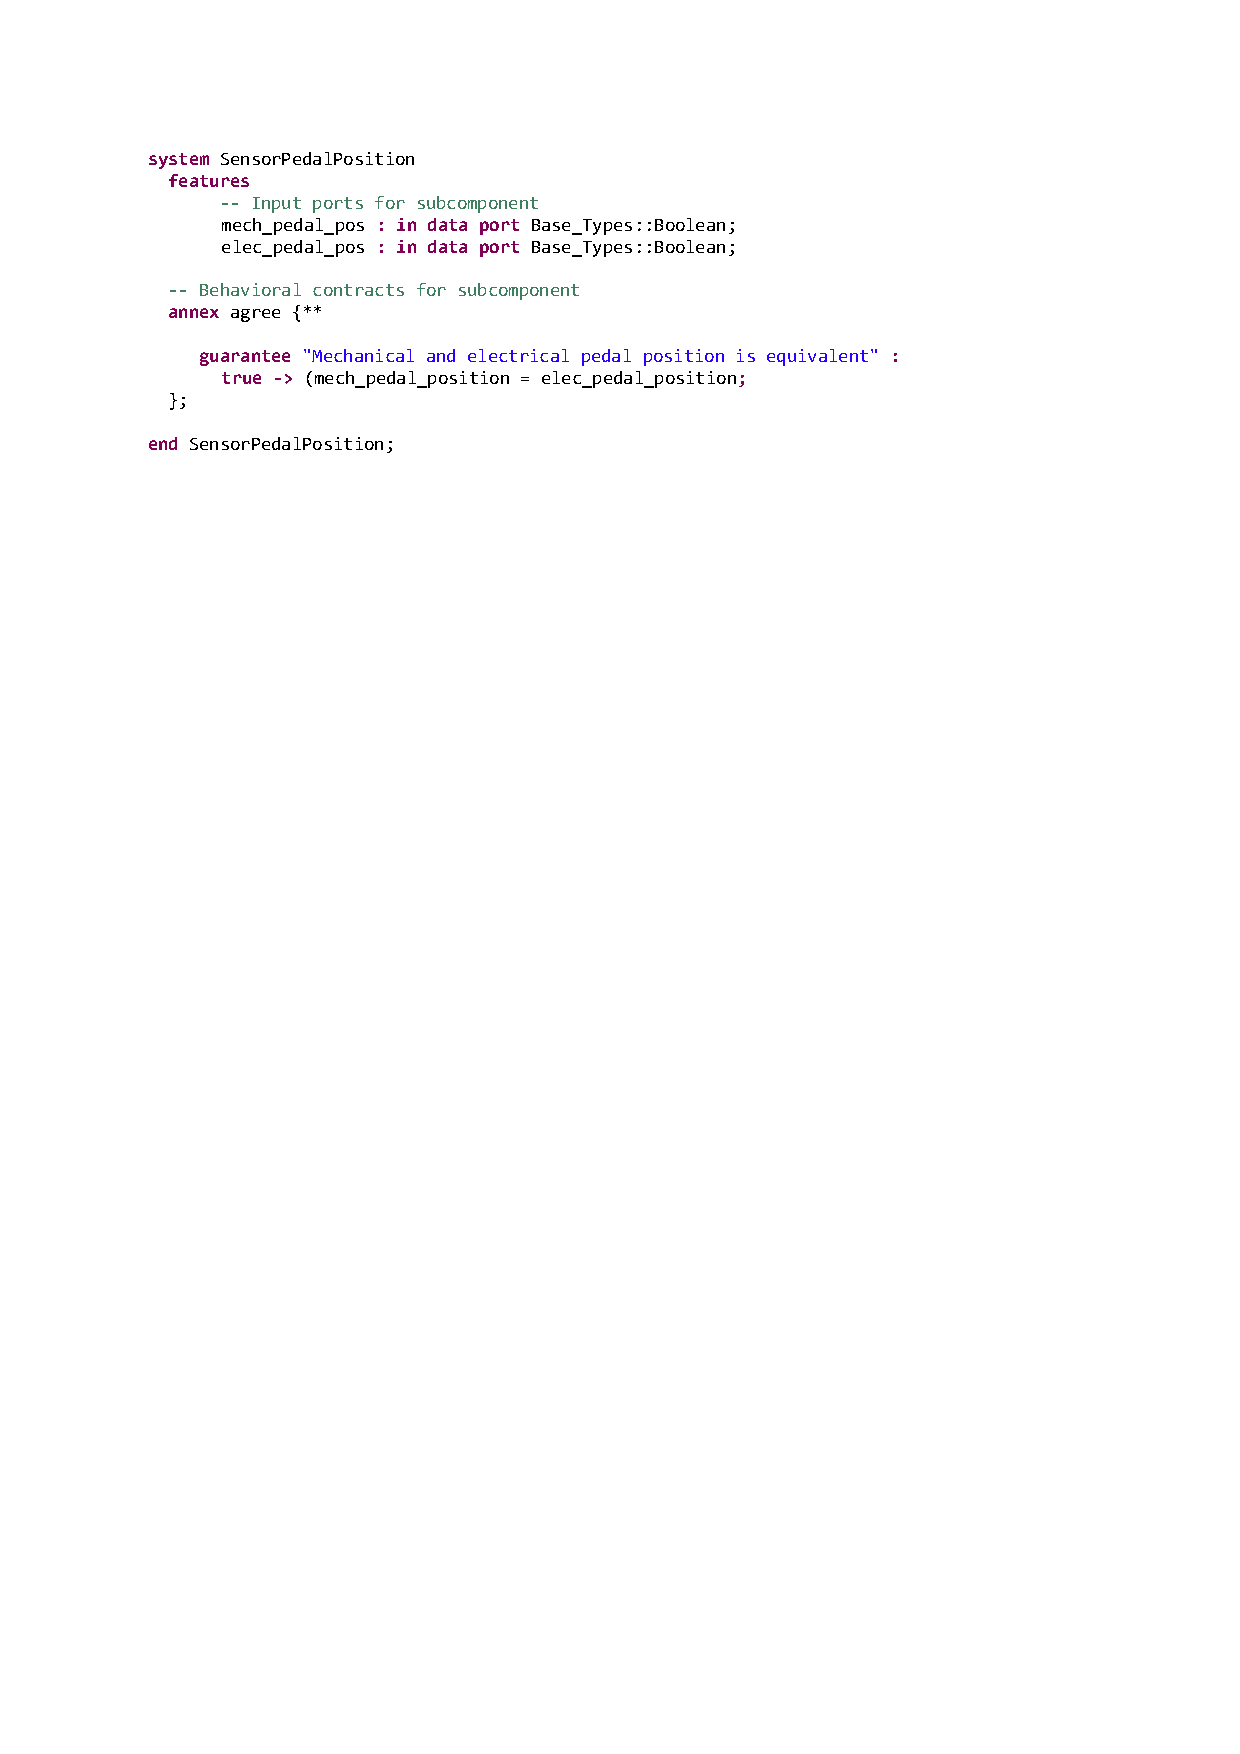
\includegraphics[trim=0 640 -10 70,clip,width=1.5\dimexpr\textwidth-2cm\relax]{images/system_sensor.pdf}
		\vspace{-0.3in}
		\caption{An AADL System Type: The Pedal Sensor}
		\label{fig:sensor}
	\end{center}
	\vspace{-0.2in}
\end{figure}

One possible failure for this sensor is inversion of its output value. This fault can be triggered with probability $5.0\times 10^{-6}$ as described in AIR6110 (in reality, the component failure probability is 
collected from hardware specification sheets).  
The Safety Annex definition for this fault is shown in Figure~\ref{fig:sensorFault}. Fault behavior is defined through the use of a fault node called \textit{inverted\_fail}.  When the fault is triggered, the nominal output of the component (\textit{elec\_pedal\_position}) is replaced with its failure value (\textit{val\_out}). 

\begin{figure}[h!]
	\hspace*{-2cm}
	%\vspace{-0.5in} 
	\begin{center}
		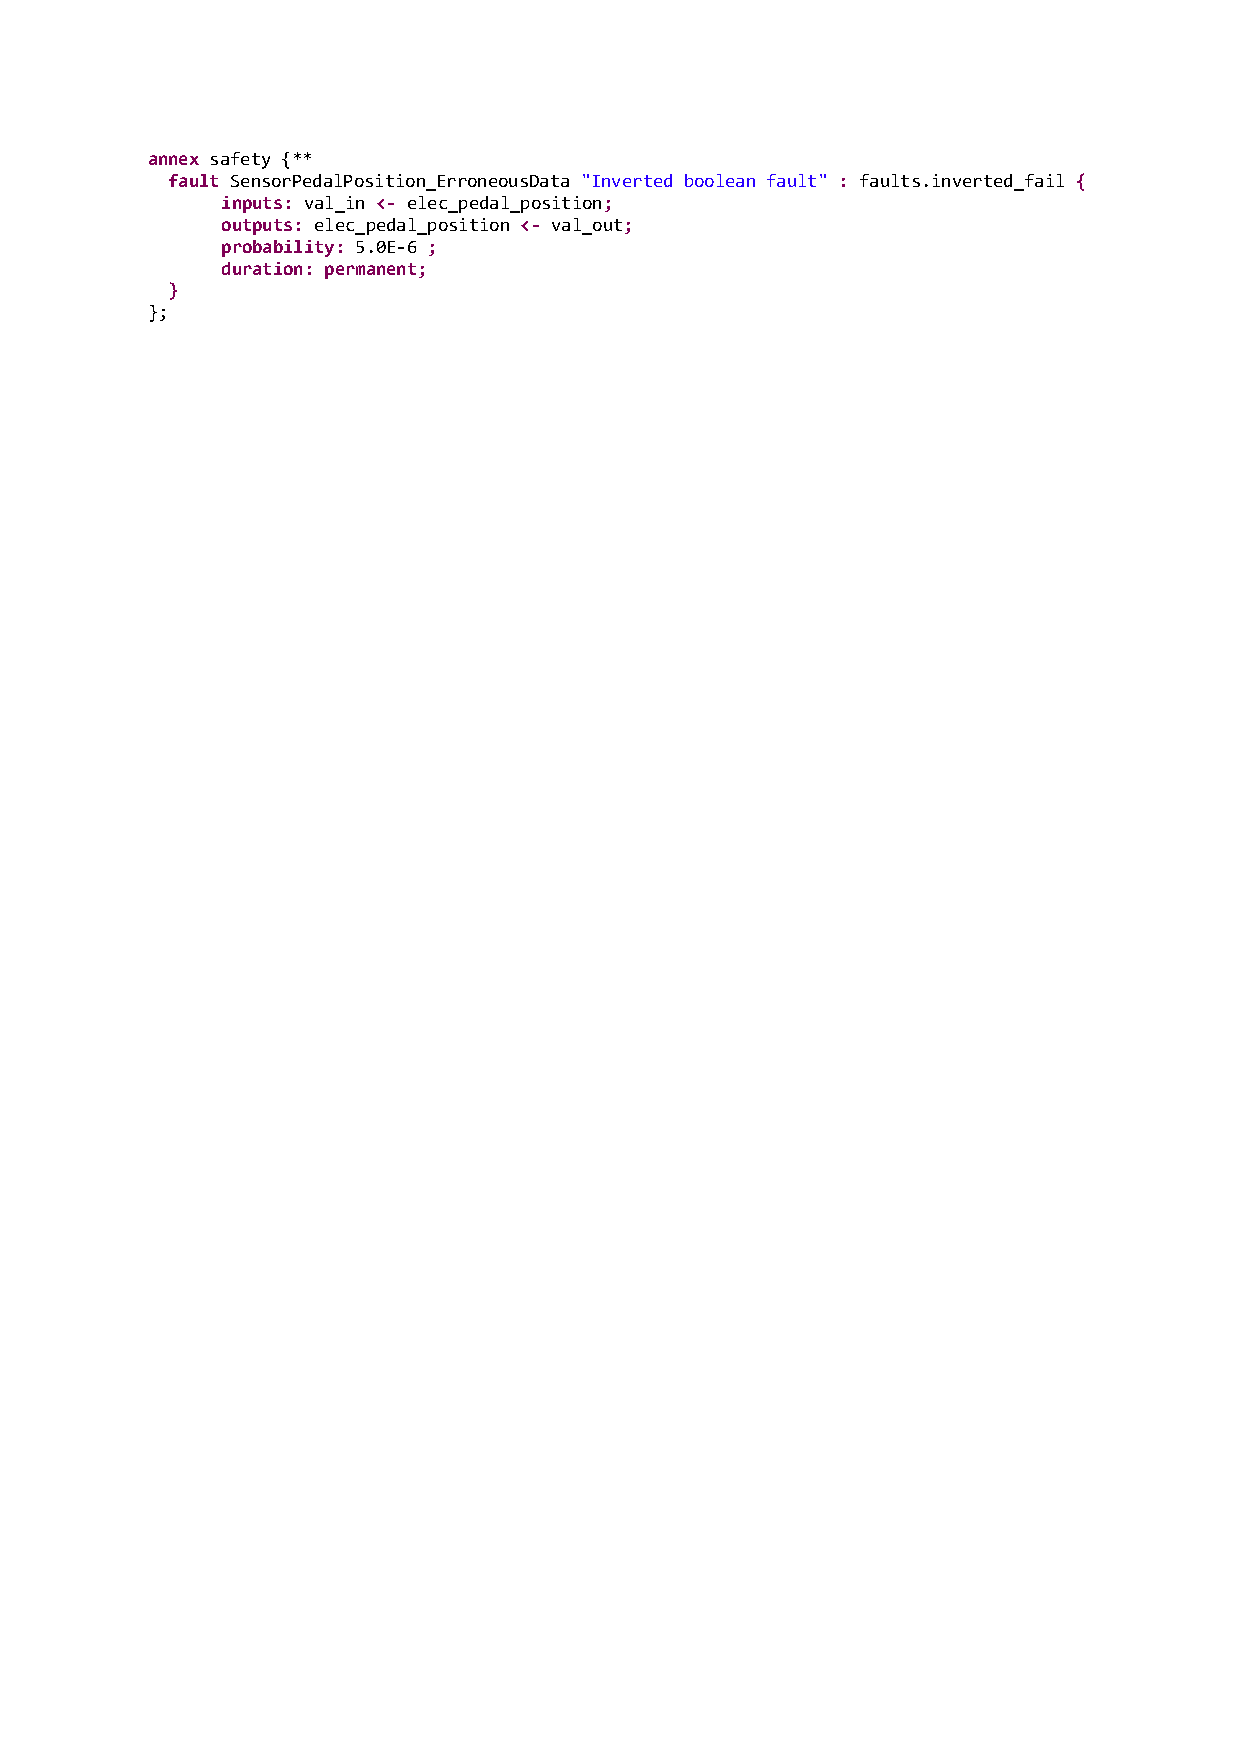
\includegraphics[trim=0 680 -10 70,clip,width=1.5\dimexpr\textwidth-2cm\relax]{images/safetyannex_sensorfault.pdf}
		\vspace{-0.2in}
		\caption{The Safety Annex for the Pedal Sensor}
		\label{fig:sensorFault}
	\end{center}
	\vspace{-0.2in}
\end{figure}

The WBS fault model expressed in the Safety Annex contains a total of 33 different fault types and 141 fault instances. The large number of fault instances is due to the redundancy in the system design and its replication to control 8 wheels.

\subsection{Implicit %Failure
	Error Propagation}
In the Safety Annex approach, faults are captured as faulty behaviors that augment the system behavioral model in AGREE contracts. No explicit %fault
error propagation is necessary since the faulty behavior itself propagates through the system just as in the nominal system model. The effects of any triggered fault are manifested through analysis of the AGREE contracts. 

On the contrary, in the AADL Error Model Annex, Version 2 (EMV2)~\cite{EMV2} approach, all errors must be explicitly propagated through each component (by applying fault types on each of the output ports) in order for a component to have an impact on the rest of the system. To illustrate the key differences between implicit %failure
error propagation provided in the Safety Annex and the explicit %failure 
error propagation provided in EMV2, we use a simplified behavioral flow from the WBS example using code fragments from EMV2, AGREE, and the Safety Annex. 

\begin{figure}[t]
	\hspace*{-2cm}
	\vspace{-0.19in}
	\centering
	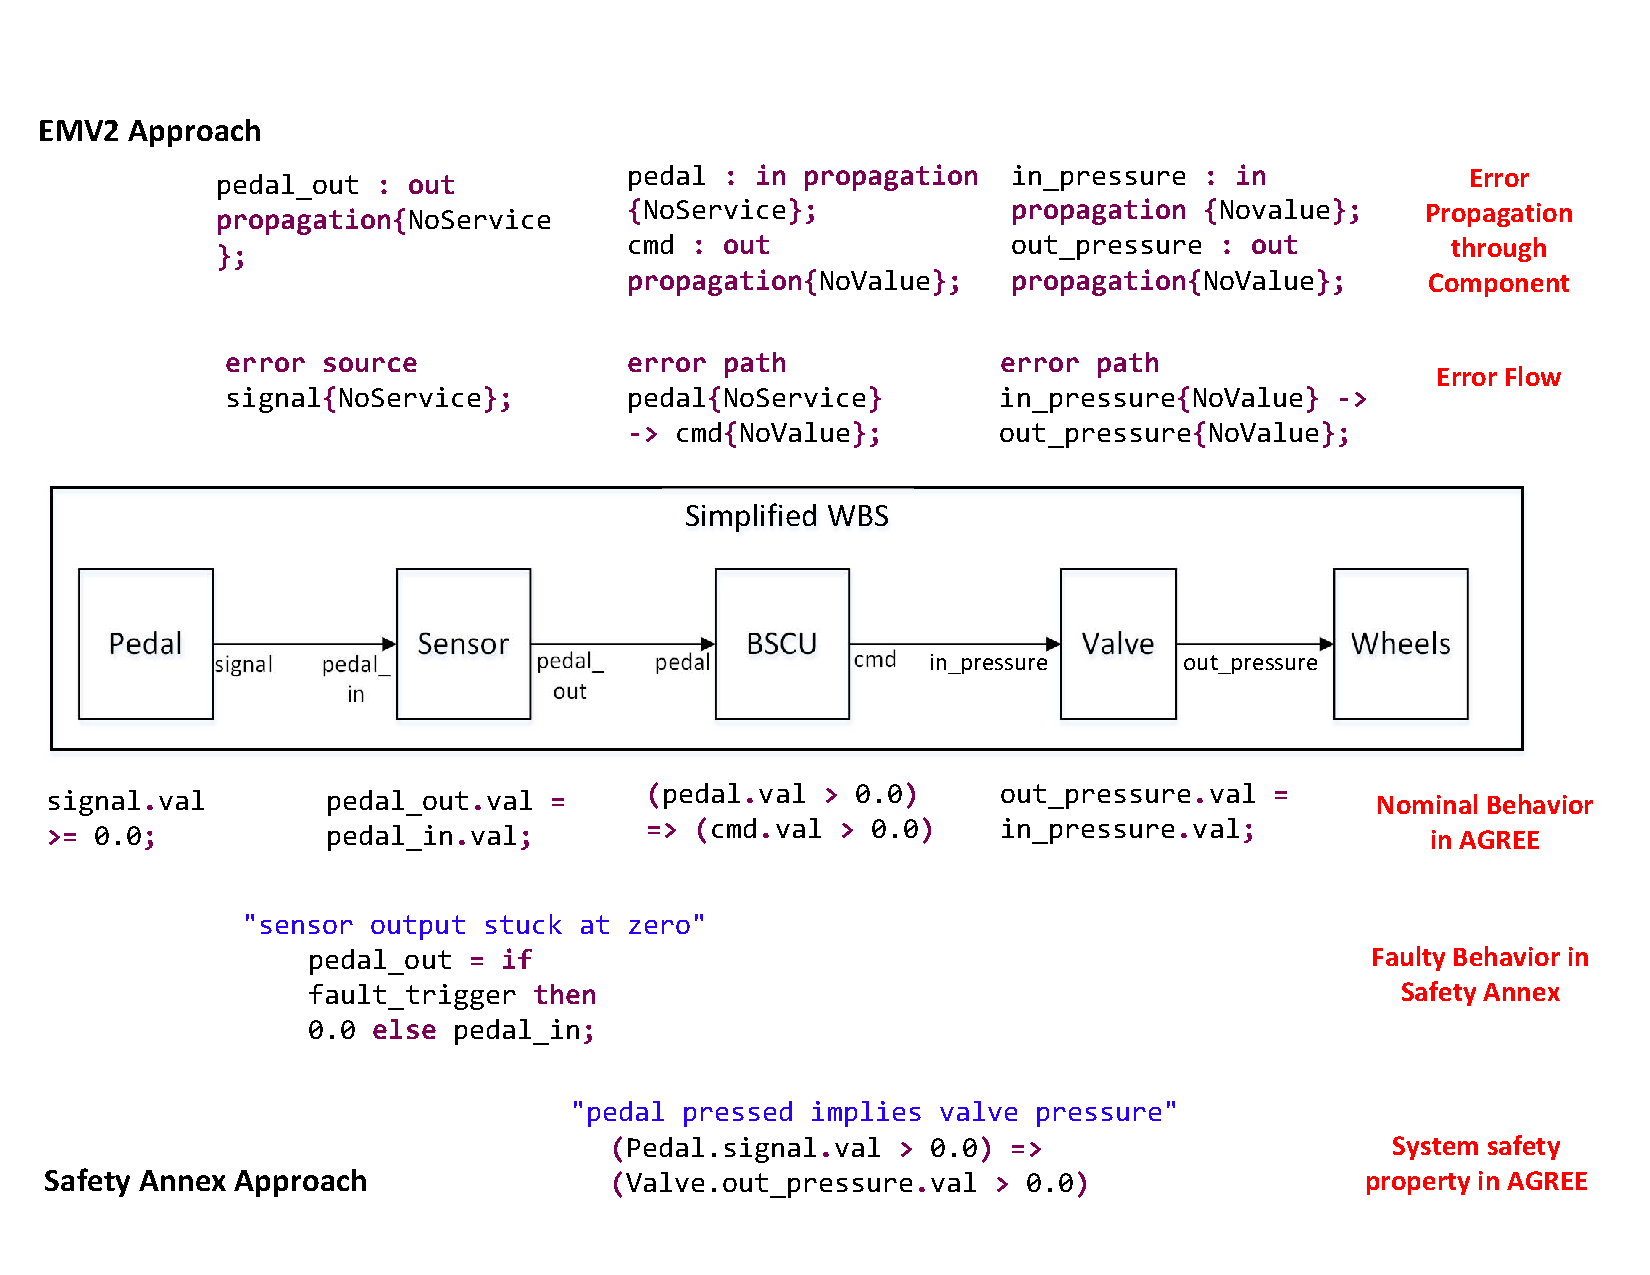
\includegraphics[trim=0 9 0 5,clip,width=\textwidth]{images/Comparison_with_EMV2.pdf}
	%\vspace{-0.3in}
	\caption{Differences between Safety Annex and EMV2}
	\label{fig:comparison_with_EMV2}
	%\vspace{-0.2in}
\end{figure} 

In this simplified WBS system, the physical signal from the Pedal component is detected by the Sensor and the pedal position value is passed to the Braking System Control Unit (BSCU) components.  The BSCU generates a pressure command to the Valve component which applies hydraulic brake pressure to the Wheels. 

In the EMV2 approach (top half of Figure~\ref{fig:comparison_with_EMV2}), the ``NoService'' fault is explicitly propagated through all of the components. These fault types are essentially tokens that do not capture any analyzable behavior. At the system level, analysis tools supporting the EMV2 annex can aggregate the propagation information from different components to compose an overall fault flow diagram or fault tree. 

When a fault is triggered in the Safety Annex (bottom half of Figure~\ref{fig:comparison_with_EMV2}), the output behavior of the Sensor component is modified. In this case the result is a ``stuck at zero'' error. The behavior of the BSCU receives a zero input and proceeds as if the pedal has not been pressed. This will cause the top level system contract to fail: {\em pedal pressed implies brake pressure output is positive}.

\begin{comment}
%\subsection{Comparison to the AADL Error Annex}

The AADL language has previously been extended to provide some fault modeling and analysis capabilities using its Error Model Annex, Version 2 (EMV2)~\cite{EMV2}.  EMV2 focuses on injection and propagation of discrete faults for generation of fault trees, rather than on analysis of system behavior in the presence of faults. 
To illustrate some of the key differences between our approach and the EMV2 approach, Figure~\ref{fig:comparison_with_EMV2} shows a simplified  behavioral flow with code fragments from EMV2, AGREE, and the Safety Annex. 

\begin{figure}[t]
	\vspace{-0.45in}
	\centering
	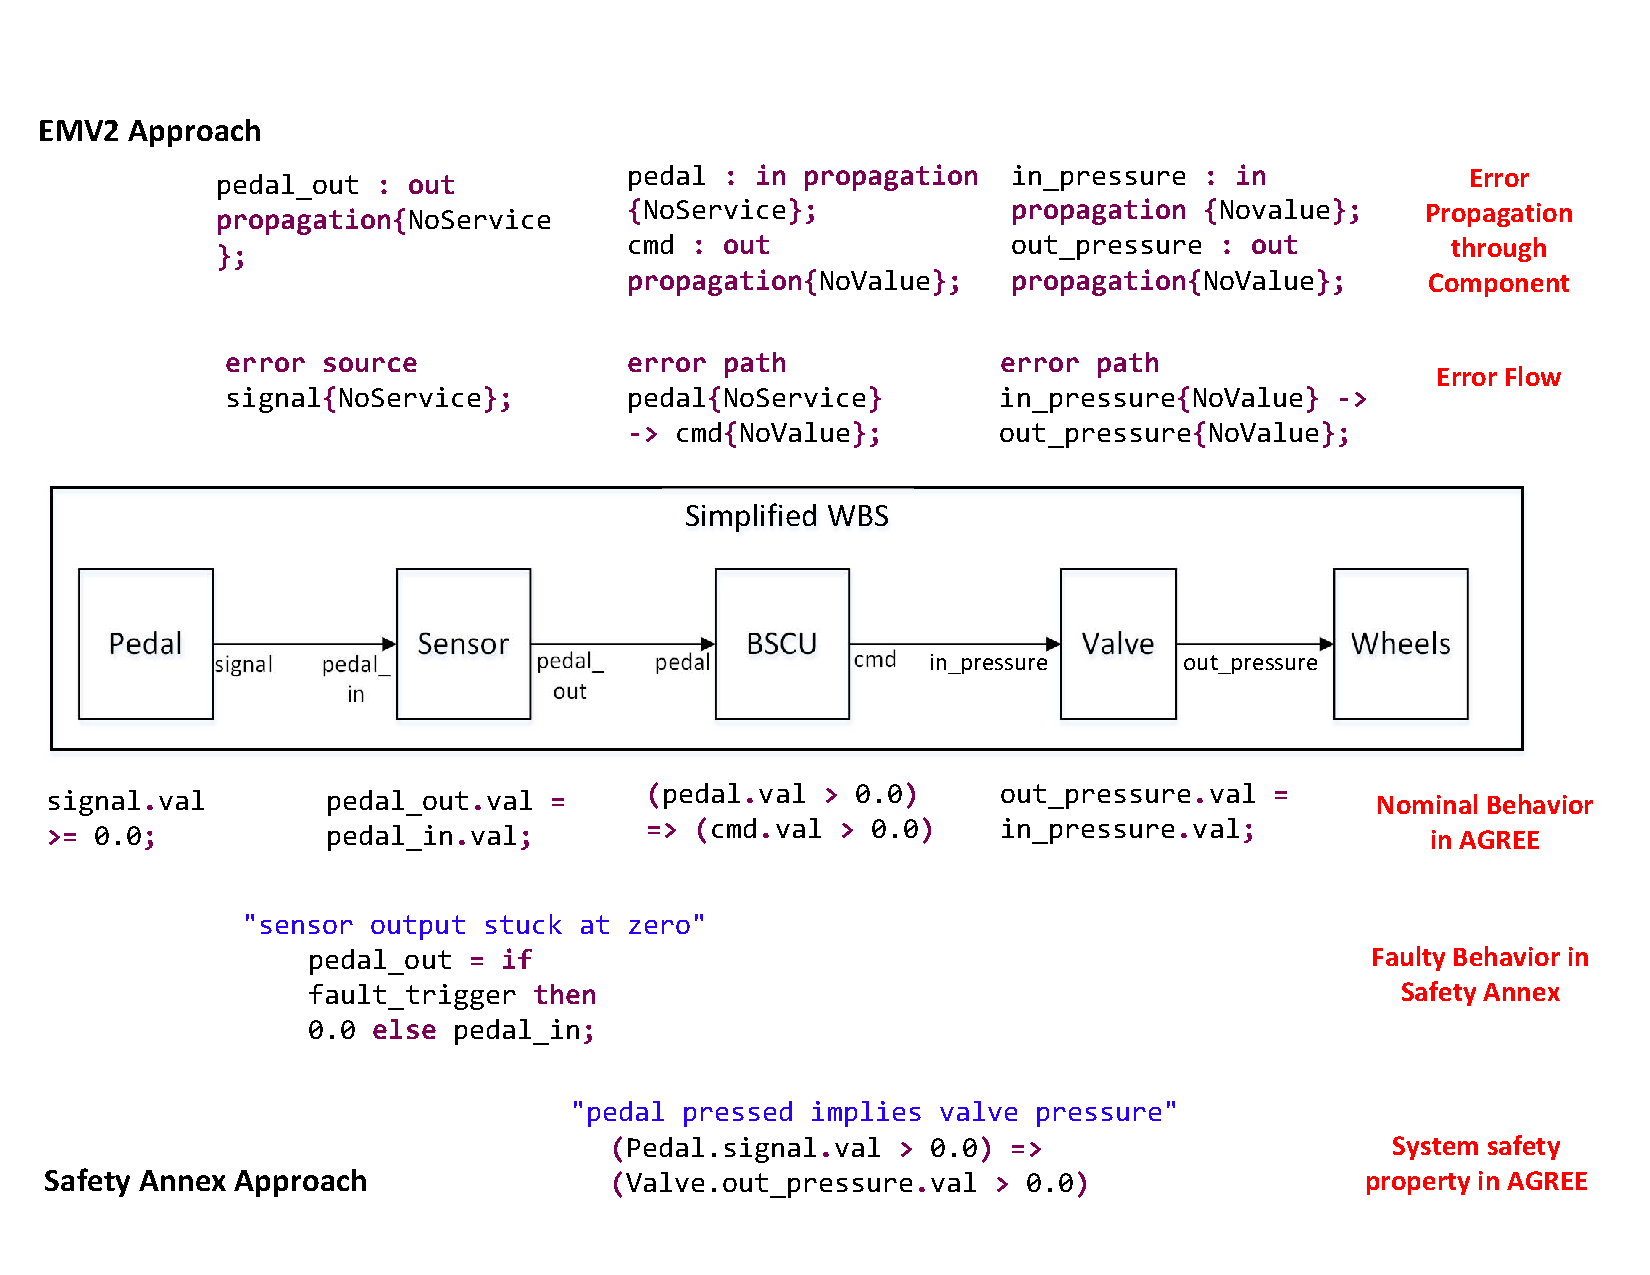
\includegraphics[trim=0 9 0 5,clip,width=\textwidth]{images/Comparison_with_EMV2.pdf}
	%\vspace{0.4in}
	\caption{Differences between Safety Annex and EMV2}
	\label{fig:comparison_with_EMV2}
\end{figure} 

In this simplified WBS system, the physical signal from the Pedal component is detected by the Sensor, and the pedal position value is passed to the Braking System Control Unit (BSCU) components.  The BSCU generates a pressure command to the Valve component which applies hydraulic brake pressure to the Wheels. 

In the EMV2 approach (top half of Figure~\ref{fig:comparison_with_EMV2}), all errors must be explicitly propagated through each component (by applying fault types on each of the output ports) in order for a component to have an impact on the rest of the system. In the example, the ``NoService'' fault is explicitly allowed by the EMV2 declarations to propagate through all of the components.  These fault types are essentially tokens that do not capture any analyzable behavior.  At the system level, analysis tools supporting the EMV2 annex can aggregate the fault flow and propagation information from different components to compose an overall fault flow diagram or fault tree.

In the Safety Annex approach (bottom half of Figure~\ref{fig:comparison_with_EMV2}), faults augment the system behavioral model through the AGREE contracts.  When a fault is triggered, the output behavior of the Sensor component is modified, in this case resulting a ``stuck at zero'' error. The behavior of the BSCU receives a zero input and proceeds as if the pedal has not been pressed. This will cause the top level system contract to fail: {\em pedal pressed implies brake pressure output is positive}. No explicit propagation is necessary since the faulty behavior propagates through the system just as in the nominal system model. The system and component failures are manifested through analysis of the AGREE contracts. 
\end{comment}

\subsection{Explicit %Failure 
	Error Propagation} 
%Faults
Failures in hardware (HW) components can trigger behavioral faults in the system components that depend on them. For example, a CPU %fault
Failure may trigger faulty behavior in the threads bound to that CPU. In addition, a %fault
failure in one HW component may trigger %faults
failure in other HW components located nearby, such as overheating, fire, or explosion
in the containment location. 
The Safety Annex provides the capability to explicitly model the impact of hardware %faults
failures on other faults, behavioral or non behavioral. The explicit propagation to non behavioral faults is similar to that provided in EMV2.

To better model %HW dependent faults 
faults at the system level dependent on HW failures, a fault model element is introduced called a \textit{hardware fault}. Users are not required to specify behavioral effects for the HW faults, nor are data ports necessary on which to apply the fault definition. An example of a model component fault declaration is shown below:
\begin{figure}[h!]
	\vspace{-0.1in}
	\begin{center}
	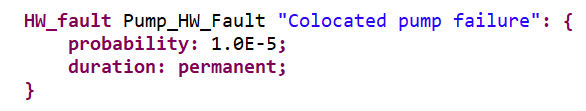
\includegraphics[width=.6\textwidth]{images/hw_fault2.png}
	\end{center}
	\vspace{-0.3in}
	%\caption{Hardware Fault Definition}
	\label{fig:hwFault}
	%\vspace{-0.2in}
	%\vspace{-0.1in}
\end{figure}

Users specify dependencies between the HW component faults and faults that are defined in other components, either HW or SW. The hardware fault then acts as a trigger for dependent faults. This allows a simple propagation from the faulty HW component to the SW components that rely on it, affecting the behavior on the outputs of the affected SW components.

%As an example, we will look yet again at the WBS. 
In the WBS example, assume that both the green and blue hydraulic pumps are located in the same compartment in the aircraft and an explosion in this compartment rendered both pumps inoperable.
%An accident took place and the green (normal) hydraulic pump took the force of an explosion. When the green hydraulic pump exploded, the pump shrapnel flew into the blue pump and it became from then on unoperable. 
The HW fault definition can be modeled first in the green hydraulic pump component as shown in Figure~\ref{fig:hwFault}. The activation of this fault triggers the activation of related faults as seen in the \textit{propagate\_to} statement shown below. % in Figure~\ref{fig:hwFaultProp}. 
Notice that these pumps need not be connected through a data port in order to specify this propagation. %Furthermore, the probability of the HW fault activation can be specified. 

\begin{figure}[h!]
	\vspace{-0.1in}
	\begin{center}
		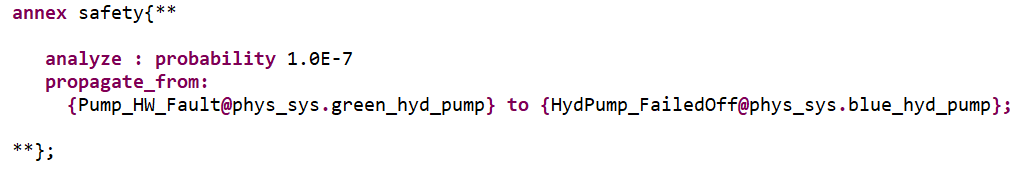
\includegraphics[width=1.0\textwidth]{images/hw_prop_stmt.png}
	\end{center}
	\vspace{-0.3in}
	%\caption{Hardware Fault Propagation Statement}
	\label{fig:hwFaultProp}
	%\vspace{-0.2in}
	%\vspace{-0.1in}
\end{figure}

The fault dependencies are specified in the system implementation where the system configuration that causes the dependencies becomes clear (e.g., binding between SW and HW components, co-location of HW components). 
%This is because fault propagations are typically tied to the way components are connected or bound together; this information may not be available when faults are being specified for individual components. Having fault propagations specified outside of a component’s fault statements also makes it easier to reuse the component in different systems. 



\subsection{Fault Analysis Statements}
%An annotation in the AADL model determines the fault analysis statement (also referred to in this report as the fault hypothesis). This may specify either a maximum number of faults that can be active at any point in execution:
The fault analysis statement (also referred to as the fault hypothesis) resides in the AADL system implementation that is selected for verification. This may specify either a maximum number of faults that can be active at any point in execution:

\begin{figure}[h!]
	\vspace{-0.1in}
	%\begin{center}
		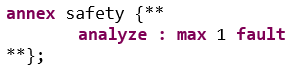
\includegraphics[width=0.4\textwidth]{images/hypothesisMaxN.png}
	%\end{center}
	\vspace{-0.1in}
	%%\caption{Max N Faults Analysis Statement}
	\label{fig:hypothesisMaxN}
\end{figure}
or that the only faults to be considered are those whose probability of simultaneous occurrence is above some probability threshold: 

\begin{figure}[h!]
	\vspace{-0.1in}
	%\begin{center}
		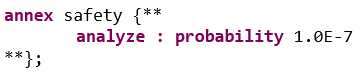
\includegraphics[width=0.5\textwidth]{images/hypothesisProb.png}
	%\end{center}
	\vspace{-0.1in}
	%\caption{Probability Analysis Statement}
	%\label{fig:hypothesisProb}
\end{figure}

Tying back to the fault tree analysis in traditional safety analysis, the former is analogous to restricting the cutsets to a specified maximum number of terms, and the latter is analogous to restricting the cutsets to only those whose probability is above some set value. In the former case, we assert that the sum of the true {\em fault\_\_trigger} variables is at or below some integer threshold.  In the latter, we determine all combinations of faults whose probabilities are above the specified probability threshold, and describe this as a proposition over {\em fault\_\_trigger} variables. 
%
With the introduction of dependent faults, active faults are divided into two categories: independently active (activated by its own triggering event) and dependently active (activated when the faults they depend on become active). The top level fault hypothesis applies to independently active faults. Faulty behaviors augment nominal behaviors whenever their corresponding faults are active (either independently active or dependently active).











\section{Byzantine Fault Modeling}
\label{sec:byzantine}
A \textit{Byzantine} or \textit{asymmetric} fault is a fault that presents different symptoms to different observers~\cite{Driscoll-Byzantine-Fault}. In our modeling environment, asymmetric faults may be associated with a component that has a 1-n output to multiple other components. In this configuration, a \textit{symmetric} fault will result in all destination components seeing the same faulty value from the source component. To capture the behavior of asymmetric faults (``different symptoms to different observers''), it was necessary to extend our fault modeling mechanism in AADL. 

\subsection{Implementation of Asymmetric Faults}
To illustrate our implementation of asymmetric faults, assume a source component A has a 1-n output connected to four destination components (B-E) as shown in Figure~\ref{fig:commNodes} under ``Nominal System.'' If a symmetric fault was present on this output, all four connected components would see the same faulty behavior. An asymmetric fault should be able to present arbitrarily different values to the connected components. 

To this end, ``communication nodes'' are inserted on each connection from component A to components B, C, D, and E (shown in Figure~\ref{fig:commNodes} under ``Fault Model Architecture.'' From the users perspective, the asymmetric fault definition is associated with component A's output and the architecture of the model is unchanged from the nominal model architecture. Behind the scenes, these communication nodes are created to facilitate potentially different fault activations on each of these connections. The fault definition used on the output of component A will be inserted into each of these communication nodes as shown by the red circles at the communication node output in Figure~\ref{fig:commNodes}.
\begin{figure}[!htb]
        \center{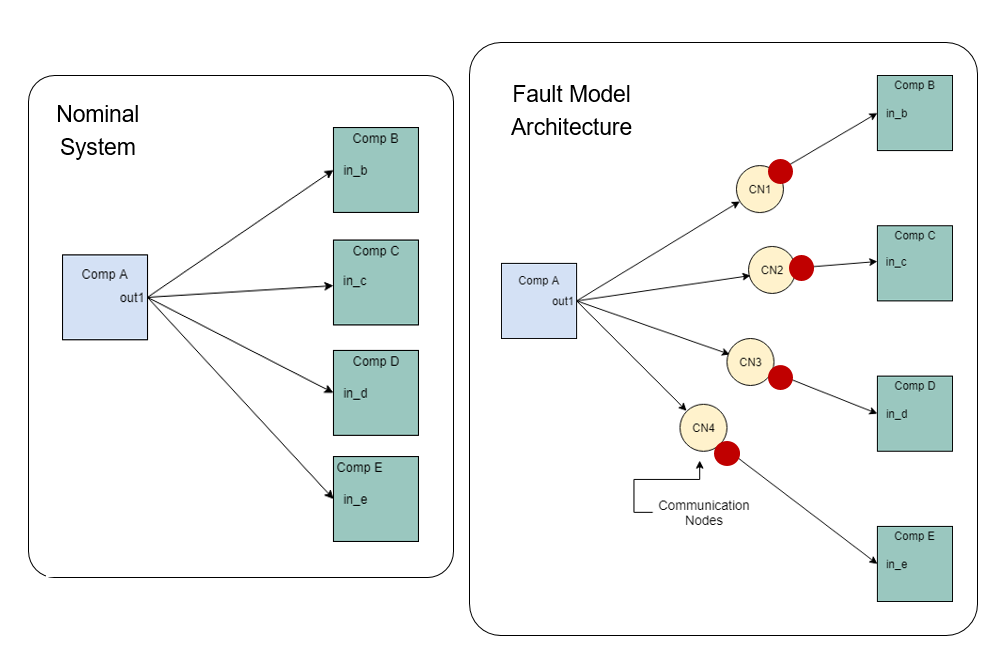
\includegraphics[width=\textwidth] {images/commNodes.png}}
        \caption{\label{fig:commNodes} Communication Nodes in Asymmetric Fault Implementation}
\end{figure}

\begin{figure}[!htb]
        \center{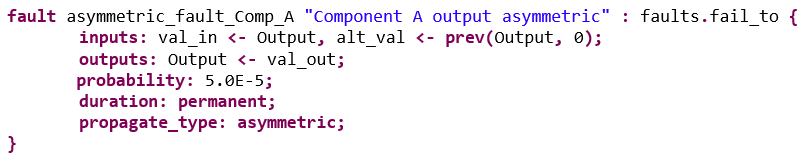
\includegraphics[width=\textwidth] {images/asymFaultDef.png}}
        \caption{\label{fig:asymFaultDef} Asymmetric Fault Definition in the Safety Annex}
\end{figure}

An asymmetric fault is defined for Component A as in Figure~\ref{fig:asymFaultDef}. This fault defines an asymmetric failure on Component A that when active, is stuck at a previous value (\textit{prev(Output, 0)}). This can be interpreted as the following: some connected components may only see the previous value of Comp A output and others may see the correct (current) value when the fault is active. This fault definition is injected into the communication nodes and which of the connected components see an incorrect value is completely nondeterministic. Any number of the communication node faults (0…all) may be active upon activation of the main asymmetric fault.

\subsection{Process ID Example}
The illustration of asymmetric fault implementation can be seen through a simple example where 4 nodes report to each other their own process ID (PID). Each node has a 1-3 connection and thus each node is a candidate for an asymmetric fault. Given this architecture, a top level contract of the system is simply that all nodes report and see the correct PID of all other nodes. Naturally in the absence of faults, this holds. But when one asymmetric fault is introduced on any of the nodes, this contract cannot be verified. What is desired is a protocol in which all nodes agree on a value (correct or arbitrary) for all PIDs. 

\subsection{The Agreement Protocol Implementation in AGREE}
In order to mitigate this problem, special attention must be given to the behavioral model. Using the strategies outlined in previous research~\cite{bracha1987asynchronous,Driscoll-Byzantine-Fault}, the agreement protocol is specified in AGREE to create a model resilient to one active Byzantine fault. 

The objective of the agreement protocol is for all correct (non-failed) nodes to eventually reach agreement on the PID values of the other nodes. There are $n$ nodes, possibly $f$ failed nodes. The protocol requires $n > 3f$ nodes to handle a single fault. The point is to achieve distributed agreement and coordinated decisions.
The properties that must be verified in order to prove the protocol works as desired are as follows: 
\begin{itemize}
	\item All correct (non-failed) nodes eventually reach a decision regarding the value they have been given.  In this solution, nodes will agree in $f+1$ time steps or rounds of communication.   
	\item If the source node is correct, all other correct nodes agree on the value that was originally sent by the source.  
	\item If the source node is failed, all other nodes must agree on some predetermined default value.  
\end{itemize}

The updated architecture of the PID example is shown in Figure~\ref{fig:PIDArch}. 
\begin{figure}[!htb]
        \center{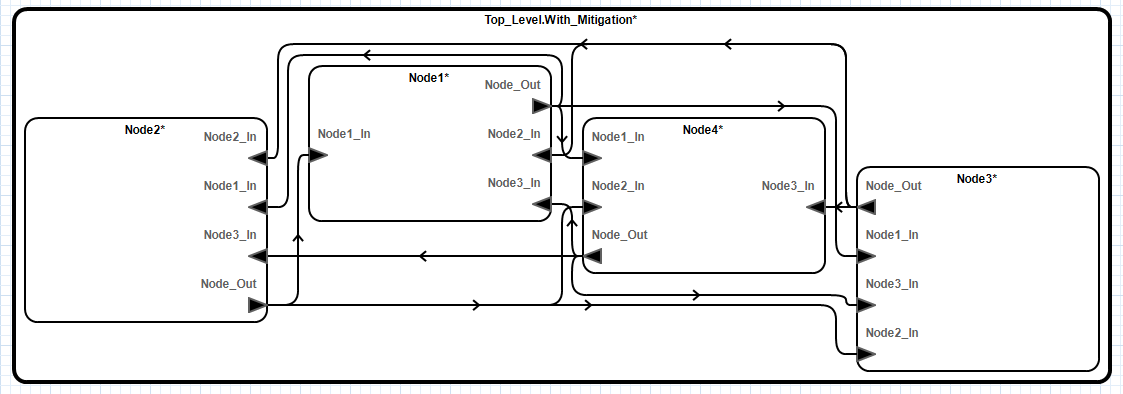
\includegraphics[width=\textwidth] {images/PIDArch.png}}
        \caption{\label{fig:PIDArch} Updated PID Example Architecture}
\end{figure}

Each node reports its own PID to all other nodes in the first round of communication. In the second round, each node informs the others what they saw in terms of %everyones
everyone's PIDs. %Thus, new connections are added for this second round of communication.
The outputs from a node are described in Figure~\ref{fig:NodeOutputsPID}. %\janet{The figure needs to be updated, as node 2 sends to node 1, 2, 3; and node 3 sends to node 1, 2, 4; and node 4 sends to node 1, 2, 3}
\begin{figure}[!htb]
        \center{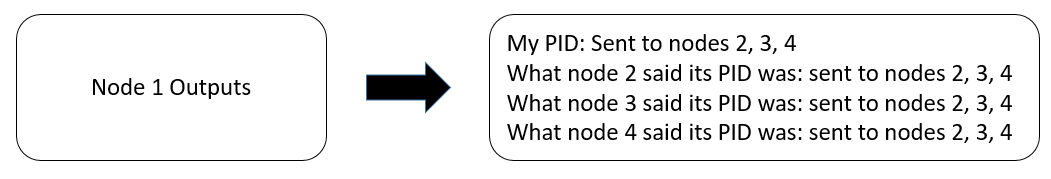
\includegraphics[width=0.9\textwidth] {images/NodeOutputsPID.png}}
        \caption{\label{fig:NodeOutputsPID} Description of the Outputs of Each Node in the PID Example}
\end{figure}
%These new connections 
These outputs are modeled as a nested data implementation in AADL and each field corresponds to a PID from a node. The AADL code fragment defining this data implementation is shown in Figure~\ref{fig:PIDNodeData}.

\begin{figure}[!htb]
        \center{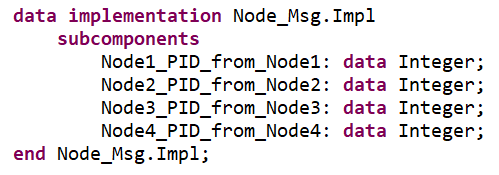
\includegraphics[width=0.7\textwidth] {images/PIDNodeData.png}}
        \caption{\label{fig:PIDNodeData} Data Implementation in AADL for Node Outputs}
\end{figure}

The fault definition for %that is inserted explicitly into the model is connected to 
each node's output and can effect the data fields arbitrarily. This is a nondeterministic fault in two ways. It is nondeterministic how many receiving nodes see incorrect values and it is nondeterministic how many of the data fields are affected by this fault. This can be accomplished through the fault definition shown in Figure~\ref{fig:PIDFaultNode} and the fault node definition in Figure~\ref{fig:PIDFaultDef}. 

\begin{figure}[!htb]
        \center{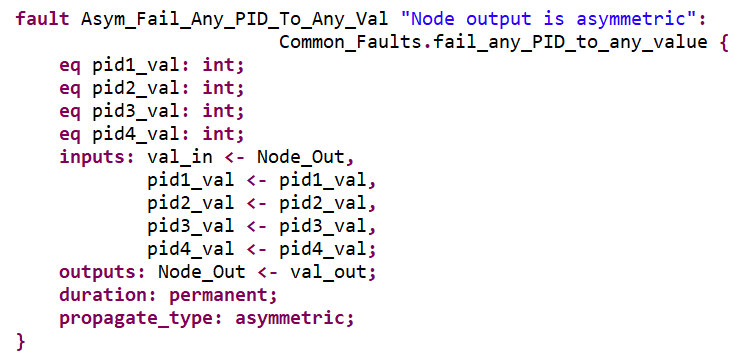
\includegraphics[width=0.9\textwidth] {images/PIDFaultNode.png}}
        \caption{\label{fig:PIDFaultNode} Fault Definition on Node Outputs for PID Example}
\end{figure}

\begin{figure}[!htb]
        \center{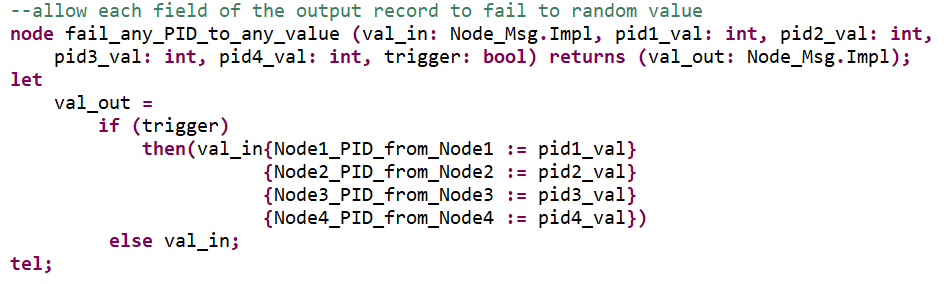
\includegraphics[width=0.9\textwidth] {images/PIDFaultDef.png}}
        \caption{\label{fig:PIDFaultDef} Fault Node Definition for PID Example}
\end{figure}

Once the fault model is in place, the implementation in AGREE of the agreement protocol is developed. As stated previously, there are two cases that must be considered in the contracts of this system. 
\begin{itemize}
	\item In the case of no active faults, all nodes must agree on the correct PID of all other nodes. 
	\item In the case of an active fault on a node, all non-failed nodes must agree on a PID for all other nodes. 
\end{itemize}

These requirements are encoded in AGREE through the use of the following contracts. Figure~\ref{fig:PIDContract1} and Figure~\ref{fig:PIDContract2} show example contracts regarding Node 1 PID. There are similar contracts for each node's PID. 
\begin{figure}[!htb]
        \center{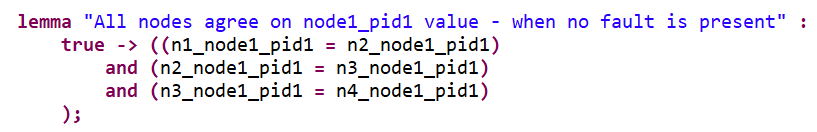
\includegraphics[width=0.9\textwidth] {images/PIDContract1.png}}
        \caption{\label{fig:PIDContract1} Agreement Protocol Contract in AGREE for No Active Faults}
\end{figure}

\begin{figure}[!htb]
        \center{\includegraphics[width=0.9\textwidth] {images/PIDCOntract2.png}}
        \caption{\label{fig:PIDContract2} Agreement Protocol Contract in AGREE Regarding Non-failed Nodes}
\end{figure}


\textbf{Referencing Fault Activation Status}
To fully implement the agreement protocol, it must be possible to describe whether or not a subcomponent is failed by specifying if any faults defined for the subcomponents is activated. In the Safety Annex, this is made possible through the use of a \textit{fault activation} statement. Users can declare boolean \textit{eq} variables in the AGREE annex of the AADL system where the AGREE verification applies to that system's implementation. %in AGREE and in the implementations Safety Annex, 
Users can then assign the activation status of specific faults to those \textit{eq} variables in Safety Annex of the AADL system implementation (the same place where the fault analysis statement resides).
%assigns this boolean \textit{eq} statement to a fault specific to a subcomponent. 
This assignment links each specified AGREE boolean variable with the 
activation status of the specified fault activation literal. %It is 
The AGREE boolean variable is true when and only when the fault is active. An example of this for the PID example is shown in Figure~\ref{fig:PID_faultActivationStmt}. %The \textit{eq} \janet{variables declared } %statements defined in AGREE are: \textit{n1\_failed, n2\_failed, n3\_failed, n4\_failed}. %, the fault name is \textit{Asym\_Fail\_Any\_PID\_To\_Any\_Value} \janet{and the fault definition applies to each of the node subcomponent instance of the top level system: \textit{node1}, \textit{node2}, \textit{node3}, \textit{node4}}. 
Each of the \textit{eq} variables declared in AGREE (i.e., \textit{n1\_failed, n2\_failed, n3\_failed, n4\_failed}) is linked to the fault activation status of the \textit{Asym\_Fail\_Any\_PID\_To\_Any\_Value} fault defined in a node subcomponent instance of the %top level 
AADL system implementation (i.e., \textit{node1}, \textit{node2}, \textit{node3}, \textit{node4}).

\begin{figure}[!htb]
        \center{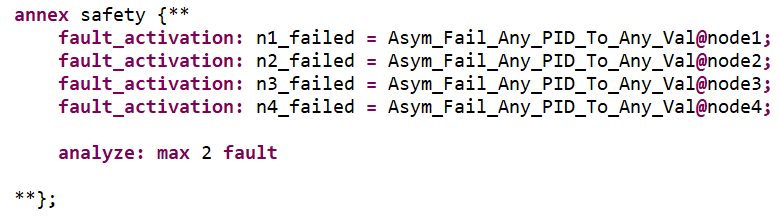
\includegraphics[width=0.9\textwidth] {images/PID_faultActivationStmt.png}}
        \caption{\label{fig:PID_faultActivationStmt} Fault Activation Statement in PID Example}
\end{figure}

\subsection{PID Example Analysis Results}
The nominal model verification shows that all properties are valid. Upon running verification of the fault model (\textit{Verify in the Presence of Faults}) with one active fault, the first four properties stating that all nodes agree on the correct value (Figure~\ref{fig:PIDContract1}) fail. This is expected since this property is specific to the case when no faults are present in the model. The remaining 4 top level properties (Figure~\ref{fig:PIDContract2}) state that all non-failed nodes reach agreement in two rounds of communication. These are verified valid when any one asymmetric fault is present. This shows that the agreement protocol was successful in eliminating a single point of asymmetric failure from the model. Furthermore, when changing the number of allowed faults to two, these properties do not hold. This is expected given the theoretical result that $3f+1$ nodes are required in order to be resilient to $f$ faults and that $f+1$ rounds of communication are needed for successful protocol implementation. %, this is not surprising. 
%\janet{Since w}e only have 4 nodes and 2 rounds of communication%. 
%\janet{, t}o be resilient to two faults would require $7$ nodes and $3$ rounds of communication. 
A summary of the results follows. 
\begin{itemize}
	\item Nominal model: All top level guarantees are verified. All nodes output the correct value and all agree. 
	\item Fault model with one active fault: The first four guarantees fail (when no fault is present, all nodes agree: shown in Figure~\ref{fig:PIDContract1}). This is expected if faults are present. The last four guarantees (all non-failed nodes agree) are verified as true with one active fault. 
	\item Fault model with two active faults: All 8 guarantees fail. This is expected since in order to be resilient up to two active faults ($f=2$), we would need $3f + 1 = 7$ nodes and $f+1 = 3$ rounds of communication. 
\end{itemize}
This model is in Github and is called PIDByzantineAgreement~\cite{SAGithub}.





\section{Implementation Overview}
\label{sec:implementation}

The safety annex is written in Java as a plug-in for the \gls{osate} \gls{aadl} toolset, which is built on Eclipse.  It is not designed as a stand-alone extension of the language, but works with behavioral contracts specified using the \gls{agree} \gls{aadl} annex~\cite{NFM2012:CoGaMiWhLaLu}. 
The architecture of the safety annex is shown in Figure~\ref{fig:plugin-arch}.

\begin{figure}
	\begin{centering}
		%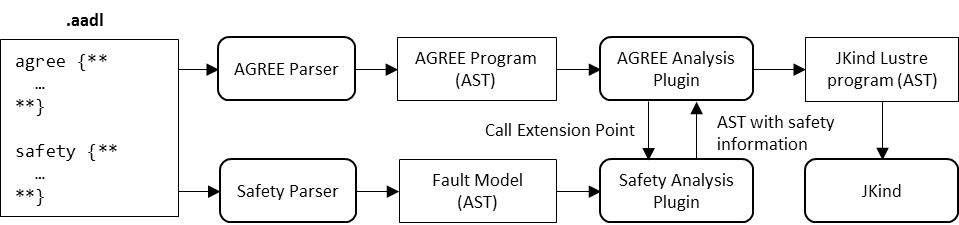
\includegraphics[trim=0 400 430 0,clip,width=0.85\textwidth]{images/arch.png}
		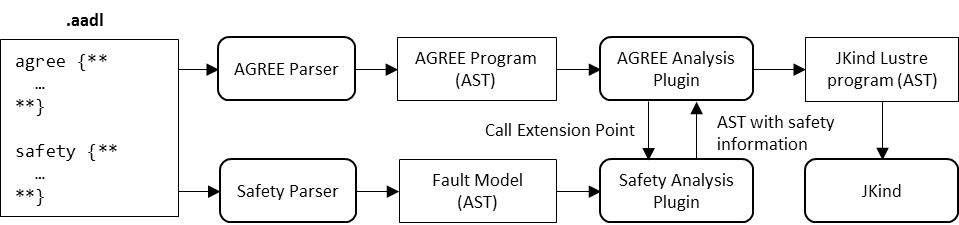
\includegraphics[width=\textwidth]{images/arch.png}
	%\vspace{-0.2in}
	\caption{Safety Annex Plug-in Architecture}
	\label{fig:plugin-arch}
	%\vspace{-0.2in}
	\end{centering}
\end{figure}

\gls{agree} contracts are used to define the nominal behaviors of system components as {\em guarantees} that hold when {\em assumptions} about the values the component's environment are met. When an \gls{aadl} model is annotated with \gls{agree} contracts and the fault model is created using the safety annex, the model is transformed through \gls{agree} into a Lustre model~\cite{Halbwachs91:IEEE} containing the behavioral extensions defined in the \gls{agree} contracts for each system component. 

%This program is intercepted by the Safety Annex plugin and fault model information is added in two ways, depending on which form of fault analysis is being run. 

%\subsection{Verification in the Presence of Faults}
When performing fault analysis, the safety annex extends the \gls{agree} contracts to allow faults to modify the behavior of component inputs and outputs. An example of a portion of an initial \gls{agree} node and its extended contract is shown in Figure~\ref{fig:lustre}. The left column of the figure shows the nominal Lustre pump definition with an \gls{agree} contract on the output. The right column shows the additional local variables for the fault (boxes 1 and 2), the assertion binding the fault value to the nominal value (boxes 3 and 4), and the fault node definition (box 5). Once augmented with fault information, the \gls{agree} model (translated into the Lustre dataflow language~\cite{Halbwachs91:IEEE}) follows the standard translation path to the model checker JKind~\cite{2017arXiv171201222G}, an infinite-state model checker for safety properties. 

\begin{figure}[h!]
	%\hspace*{-2cm}
	%\vspace{-0.3in} 
	\begin{centering}
		%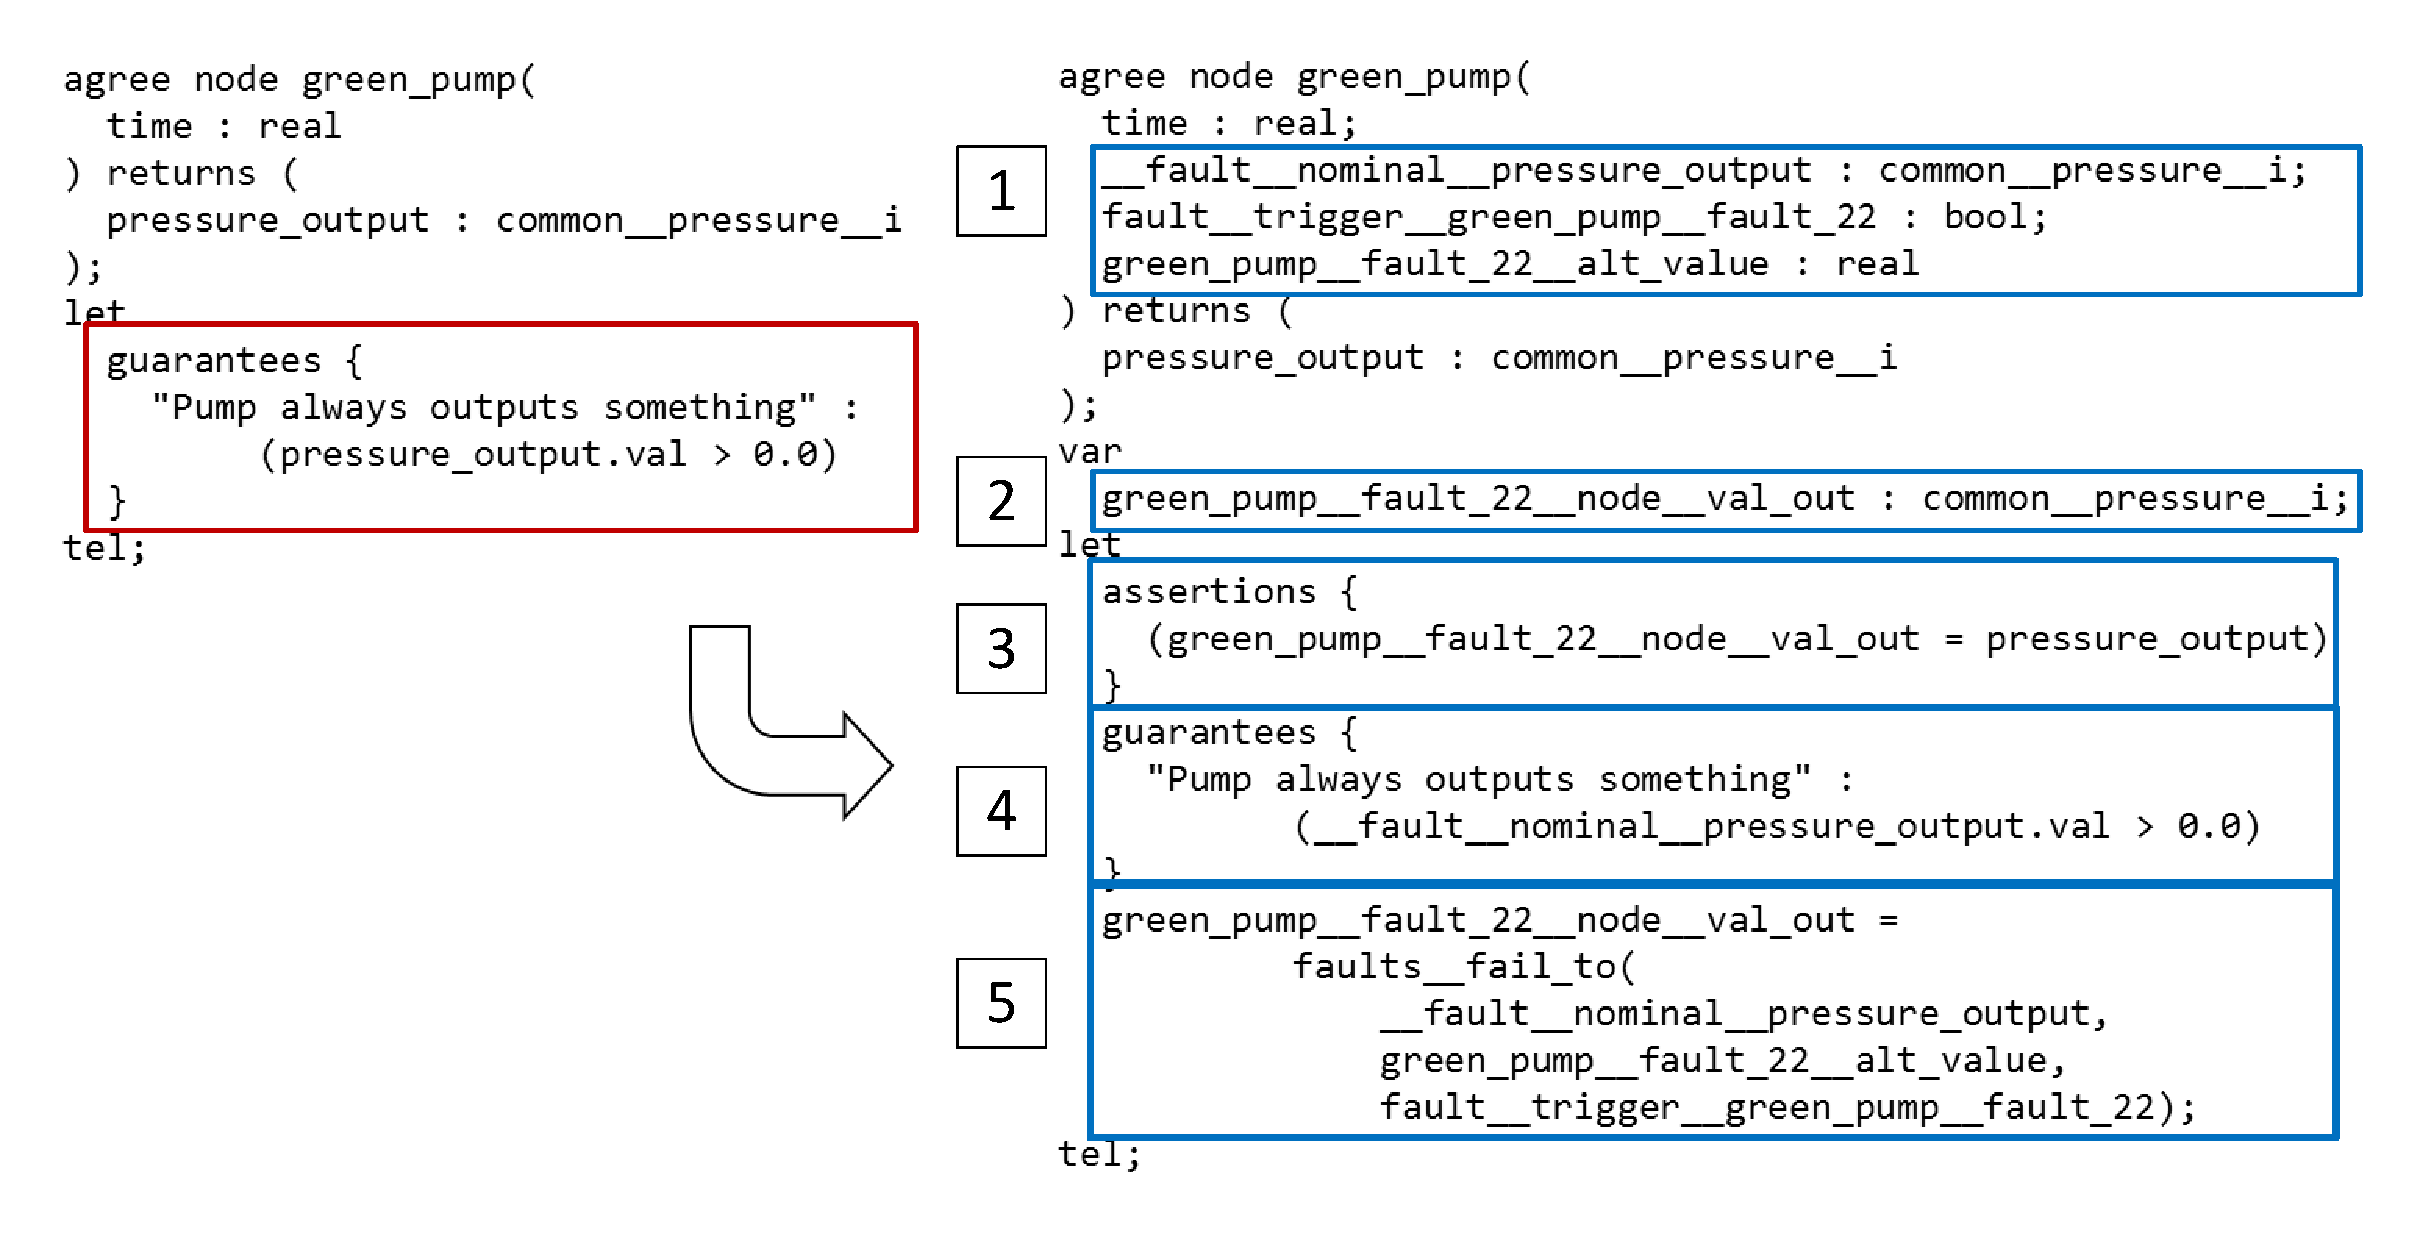
\includegraphics[trim=0 690 -10 70,clip,width=1.5\dimexpr\textwidth-2cm\relax]{images/lustre.pdf}
		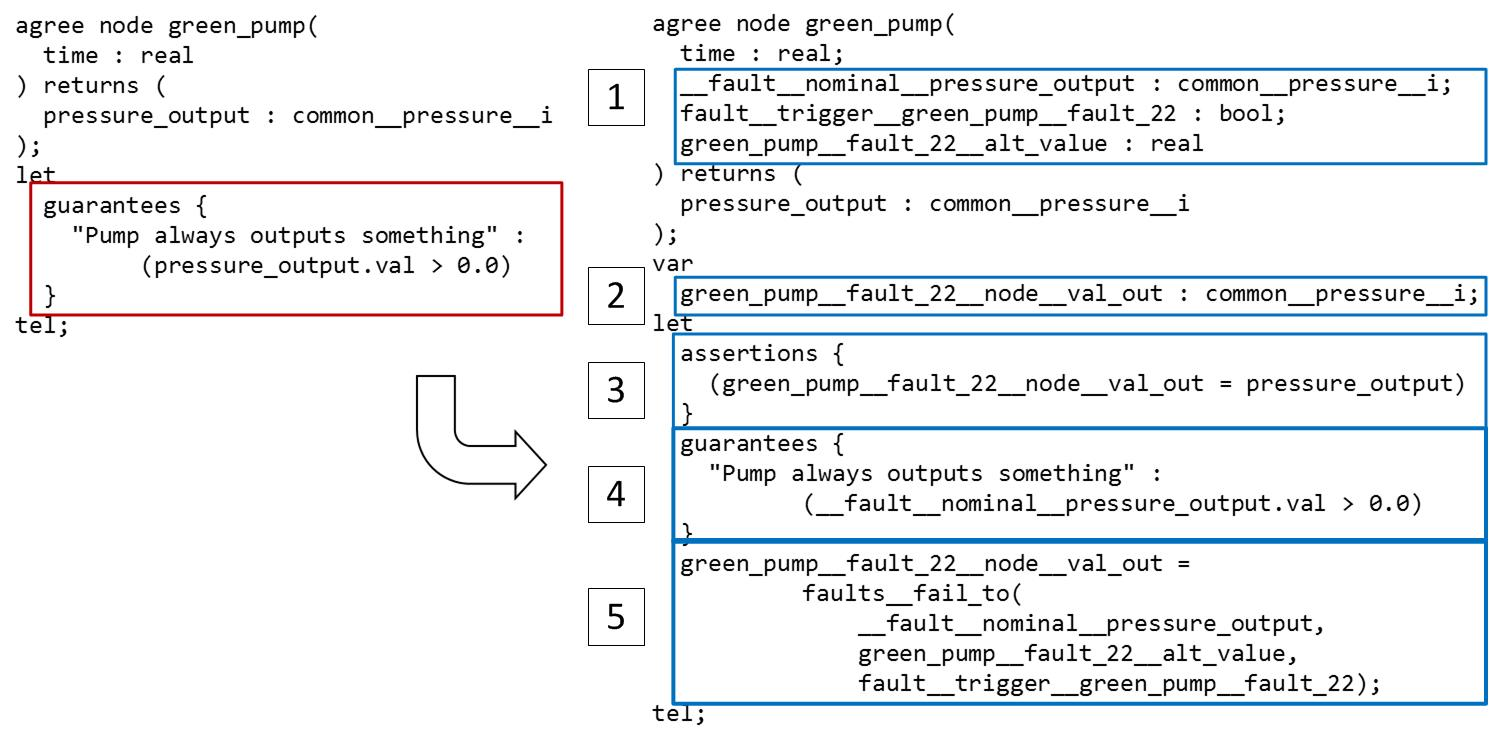
\includegraphics[width=\textwidth]{images/lustre.jpg}
		%\caption{Nominal AGREE node and its extension with faults}
		\caption{Nominal AGREE Node and Extension with Faults}
		\label{fig:lustre}
	%\vspace{-0.3in}
	\end{centering}
\end{figure}

The Lustre formulae are represented in JKind as a transition system, and reasoning is performed using $k$-induction. When performing safety analysis over the model, each fault is defined as an {\em activation literal} and given limited constraint. If the assignment to an activation literal is {\em true}, this corresponds to an active fault and potentially violated guarantee. If that assignment violates a guarantee, then this violation will be reflected in the analysis results. At a system level, it can be seen if a violated guarantee will in turn violate the top level property. Hence it is seen how active faults at leaf level components violate the system level properties. 
 
This analysis approach allows for implicit propagation of violations throughout the system. It also allows for arbitrary temporal activations of faults. There are no explicit constraints put on faults stating when an activation can occur, which allows the model checking procedure free reign to activate the faults at the worst possible times. If there are dependencies regarding fault activations, these are handled through the use of explicit error propagations (see Section~\ref{sec:fault_modeling}). While the model checker may choose various permutations of fault activation, these permutations of faults in terms of exposure time and order of occurrence are not part of the minimal cut set output of this analysis. 

The main constraint put on the model checker in terms of the activation of faults consist of {\em fault hypothesis statements}. These constrain the model by stating either the number of faults that may be active at once, or the overall probability threshold that is allowed. In the latter case, each fault has an associated probability; assuming independence, the probability of a set of faults occurring should not be less than the threshold defined. 

There are two different types of fault analysis that can be performed on a fault model: verification in the presence of faults or the generation of minimal cut sets. The Safety Annex plugin intercepts the AGREE program and adds fault model information depending on which type of fault analysis is being run.

\textbf{Verification in the Presence of Faults}: This analysis returns a counterexample if any guarantee or system level property is violated by active faults in the system. The counterexample shows a concrete scenario why a property is violated, with assignments to each signal in the model by the model checker, possibly over a multi-step progression. The augmentation from Safety Annex to the \gls{agree} program includes traceability information so that when counterexamples are displayed to users, the active faults for each component are visualized.

\textbf{Generate Minimal Cut Sets}: This analysis collects all minimal sets of fault combinations that can cause violation of a property.
%\subsection{Generate Minimal Cut Sets}
Given a complex model, it is often useful to extract traceability information related to the proof, in other words, which portions of the model were necessary to construct the proof. An algorithm was introduced by Ghassabani, et. al. to provide Inductive Validity Cores (IVCs) as a way to determine which model elements are necessary for the inductive proofs of the safety properties for sequential systems~\cite{GhassabaniGW16}. Given a safety property of the system, a model checker can be invoked in order to construct a proof of the property. The IVC generation algorithm extracts traceability information from the proof process and returns a minimal set of the model elements required in order to prove the property. Later research extended this algorithm in order to produce all Minimal Inductive Validity Cores (All-MIVCs) to provide a full enumeration of all minimal set of model elements necessary for the inductive proofs of a safety property~\cite{Ghassabani2017EfficientGO}. 

In this approach, we use the All-MIVCs algorithm to compute the minimal set of model elements (including component contracts and fault activation literals) necessary to prove the top level property, and transform them to minimal sets of faults for the violation of the top level property~\cite{nasaFinalReport}. 

To access the tool plugin, user manual, or models, see the repository located at \small \url{https://github.com/loonwerks/AMASE/}. \normalsize 

























\section{Analysis of the Model}
\label{sec:fault_analysis_2}
In this section we describe results from the nominal model analysis and the fault analysis.  

\subsection{Nominal Model Analysis}
Before performing fault analysis, users should first check that the safety properties are satisfied by the nominal design model. This analysis can be performed monolithically or compositionally in AGREE. Using monolithic analysis, the contracts at the lower levels of the architecture are flattened and used in the proof of the top level safety properties of the system. Compositional analysis, on the other hand, will perform the proof layer by layer top down, essentially breaking the larger proof into subsets of smaller problems. For a more comprehensive description of these types of proofs and analyses, see additional publications related to AGREE \cite{cofer2012compositional,QFCS15:backes} 

The WBS has a total of 13 safety properties at the top level that are supported by subcomponent assumptions and guarantees. These are shown in Table \ref{tab:safetyProperties}. Given that there are 8 wheels, contract S18-WBS-0325-wheelX is repeated 8 times, one for each wheel. The behavioral model in total consists of 36 assumptions and 246 supporting guarantees.

\begin{table}[]
\begin{tabular}{@{}ll}
\toprule
\textbf{S18-WBS-R-0321} \\Loss of all wheel braking during landing or RTO shall be less than $5.0 \times 10^{-7}$ per flight.                                    \\ \midrule 
\textbf{S18-WBS-R/L-0322}  \\ Asymmetrical loss of wheel braking (Left/Right) shall be less than $5.0 \times 10^{-7}$ per flight. \\ \midrule
\textbf{S18-WBS-0323} \\ Never inadvertent braking with all wheels locked shall be less than $1.0 \times 10^{-9}$ per takeoff.                                                                                                                                                                                                               \\ \midrule
\textbf{S18-WBS-0324}  \\ Never inadvertent braking with all wheels shall be less than $1.0 \times 10^{-9}$ per takeoff.                                                                                                            \\ \midrule
\textbf{S18-WBS-0325-wheelX} \\ Never inadvertent braking of wheel X shall be less than $1.0 \times 10^{-9}$ per takeoff.                                                                                                           .                                                                                                                 \\ \bottomrule
\end{tabular}
\caption{Safety Properties of WBS}
\label{tab:safetyProperties}
\end{table}  

\subsection{Fault Model Analysis}
There are two main options for fault model analysis using the Safety Annex. The first option injects faulty behavior allowed by faulty hypothesis into the AGREE model and returns this model to JKind for analysis. This allows for the activity of faults within the model and traceability information provides a way for users to view a counterexample to a violated contract in the presence of faults. The second option is used to generate minimal cut sets for the model. The model is annotated with fault activation that are constrained to false as well as intermediate level guarantees as model elements for consideration for the all Minimal Inductive Validity Cores (All-MIVCs)
algorithm. The All-MIVCs traces the minimal set of model elements used to produce minimal cut sets and is described in Section~\ref{sec:theory}. This subsection presents these options and discusses the analytical results obtained. 

\subsubsection{Verification in the Presence of Faults: Max N Analysis}
Using a max number of faults for the hypothesis, the user can constrain the number of simultaneously active faults in the model. The faults are added to the AGREE model for the verification. Given the constraint on the number of possible simultaneously active faults, the model checker attempts to prove the top level properties given these constraints. If this cannot be done, the counterexample provided will show which of the faults (N or less) are active and which contracts are violated. 

The user can choose to perform either compositional or monolithic analysis using a max N fault hypothesis. In compositional analysis, the analysis proceeds in a top down fashion. To prove the top level properties, the properties in the layer directly beneath the top level are used to perform the proof. The analysis proceeds in this manner. Users constrain the maximum number of faults within each layer of the model by specifying the maximum fault hypothesis statement to that layer. If any lower level property failed due to activation of faults, the property verification at the higher level can no longer be trusted because the higher level properties were proved based on the assumption that the direct sub-level contracts are valid. This form of analysis is helpful to see weaknesses in a given layer of the system. 

In monolithic analysis the layers of the model are flattened, which allows a direct correspondence between all faults in the model and their effects on the top level properties. As with compositional analysis, a counterexample shows these N or less active faults. 

\subsubsection{Verification in the Presence of Faults: Probabilistic Analysis} 
Given a probabilistic fault hypothesis, this corresponds to performing analysis with the combinations of faults whose occurrence probability is less than the probability threshold. This is done by inserting assertions that allow those combinations in the Lustre code. If the model checker proves that the safety properties can be violated with any of those combinations, one of such combination will be shown in the counterexample. 

Probabilistic analysis done in this way must utilize the monolithic AGREE option. For compositional probabilistic analysis, see Section~\ref{sec:prob_generate}.

To perform this analysis, it is assumed that the non-hardware faults occur independently and possible combinations of faults are computed and passed to the Lustre model to be checked by the model checker. As seen in Algorithm 1, the computation first removes all faults from consideration that are too unlikely given the probability threshold. The remaining faults are arranged in a priority queue $\mathcal{Q}$ from high to low. Assuming independence in the set of faults, we take a fault with highest probability from the queue (step 5) and attempt to combine the remainder of the faults in $\mathcal{R}$ (step 7). If this combination is lower than the threshold (step 8), then we do not take into consideration this set of faults and instead remove the tail of the remaining faults in $\mathcal{R}$. 
 
\begin{algorithm}[H]
	% \KwData{this text}
	% \KwResult{how to write algorithm with \LaTeX2e }
	$\mathcal{F} = \{\}$ : fault combinations above threshold \;
	$\mathcal{Q}$ : faults, $q_i$, arranged with probability high to low \;
	$\mathcal{R} = \mathcal{Q}$ , with $r \in \mathcal{R}$\;
	\While{$\mathcal{Q} \neq \{\} \land \mathcal{R} \neq \{\}$ }{
		$q =$ removeTopElement($\mathcal{Q}$) \;
		\For{$i=0:|\mathcal{R}|$}{
			$prob = q \times r_i$ \;
			\eIf{prob $<$ threshold}{
				removeTail($\mathcal{R}, j=i:|\mathcal{R}|$)\;
			}{
				add($\{q, r_i\}, \mathcal{Q}$)\;
				add($\{q, r_i\}, \mathcal{F}$)\;
			} % end if else
		} % end for
	} % end while
	\caption{Monolithic Probability Analysis}
	\label{alg:prob_monolithic}
\end{algorithm}
In this calculation, we assume independence among the faults, but in the Safety Annex it is possible to define dependence between faults using a fault propagation statement. After fault combinations are computed using Algorithm~\ref{alg:prob_monolithic}, the triggered dependent HW faults are added to the combination as appropriate. The dependencies are implemented in the \textit{Verify in the Presence of Faults} options for analysis, but not yet implemented in the \textit{Generate Minimal Cut Sets} analysis options.

\subsubsection{Generate Minimal Cut Sets: Max N Analysis}
\label{sec:maxN_generate}
As described in Section~\ref{sec:implementation}, \textit{Generate Minimal Cut Sets} analysis uses the All-MIVCs algorithm to provide a full enumeration of all minimal set of model elements necessary for the proof of each top-level safety property in the model, and then transforms all MIVCs into all minimal cut sets. In Max N analysis, the minimal cut sets are pruned to include only those with at cardinality less or equal to the max N number specified in the fault hypothesis and displayed to the user.

Generate MinCutSet analysis was performed on the Wheel Brake System and results are shown in Table~\ref{tab:wbs_maxN_results}. Notice in Table~\ref{tab:wbs_maxN_results}, the label across the top row refers to the cardinality (C) and how many cut sets of that cardinality. When the analysis is run, the user specifies the value N. This gives cut sets of cardinality \textit{less than or equal to} N. (For the full text of the properties, see Table~\ref{tab:safetyProperties}.)

\begin{center}
\begin{table}[h]
    \begin{tabular}{ | l | l | l | l | l | l | l | l |}
    \hline
    \textbf{Property} & $\bm{c = 1}$ & $\bm{c = 2}$ & $\bm{c = 3}$ & $\bm{c = 4}$ 
		& $\bm{c = 5}$ & $\bm{c = 6}$ & $\bm{c = 7+}$  \\ \hline \hline
    R-0321 & 6 & 0 & 0 & 1& 144&7776 &- \\ \hline
    R-0322 & 32 & 0 & 0 &0 &0 &0 &- \\ \hline
    L-0322 & 32 & 0 & 0 &0 &0 &0 &- \\ \hline
    0323 & 90 & 0 & 0 &0 &0 &0 &- \\ \hline
    0324 & 8 & 3,401 & 6,800 &66,472 & 435,358&1,892,832 &- \\ \hline
    0325-WX & 20 & 0 & 0 &0 &0 & 0&- \\ \hline
    \end{tabular}
    \caption{WBS MinCutSet Analysis Results for Cardinality $c$}
    \label{tab:wbs_maxN_results}
\end{table}
\end{center}



Due to the increasing number of possible fault combinations at $N=6$, the computational time increases quickly. The WBS analysis was only run to $N=6$ for this reason. 

\subsubsection{Generate Minimal Cut Sets: Probabilistic Analysis}
\label{sec:prob_generate}
Both probabilistic analysis and max N analysis use the same minimal cut set generation algorithm, except that in probabilistic analysis, the minimal cut sets are pruned to include only those fault combinations whose probability of simultaneous occurrence exceed the given threshold in the probability hypothesis. Note that with probablistic hypothesis, \textit{Verify in the Presence of Faults} is performed using only monolithic analysis, but generating minimal cut sets is performed using compositional analysis.


The probabilistic analysis for the WBS was given a top level threshold of $1.0 \times 10^{-9}$ as stated in AIR6110. The faults associated with various components were all given probability of occurrence compatible with the discussion in this same document. 

As shown in Table~\ref{tab:wbs_prob_results}, the number of allowable combinations drops considerably when given probabilistic threshold as compared to just fault combinations of certain cardinalities. For example, one contract (inadvertent wheel braking of all wheels) had over a million minimal cut sets produced when looking at it in terms of max N analysis, but after taking probabilities into account, it is seen that only one combination of faults can violate this property. (For the full text of the properties, see Table~\ref{tab:safetyProperties}.)

\begin{center}
\begin{table}[h]
    \begin{tabular}{ | l | l | l | l | l | l | l | l | l |}
    \hline
    \textbf{Property} & $\bm{c = 1}$ & $\bm{c = 2}$ & $\bm{c = 3}$ & $\bm{c = 4}$ 
		& $\bm{c = 5}$ & $\bm{c = 6}$ & $\bm{c = 7}$ & $\bm{c = 8}$  \\ \hline \hline
    R-0321 & 0 & 0 & 0 & 0 & 0 & 0 & 0 & 0 \\ \hline
    R-0322 & 32 & 0 & 0 &0 &0 &0 &0& 0  \\ \hline
    L-0322 & 32 & 0 & 0 & 0 & 0 & 0 & 0 & 0  \\ \hline
    0323 & 90 & 0 & 0 & 0 & 0 & 0 & 0 & 0  \\ \hline
    0324 & 0 & 1 & 0 & 0 & 0 & 0 & 0 & 0  \\ \hline
    0325-WX & 20 & 0 & 0 &0 &0 & 0 & 0 & 0  \\ \hline
    \end{tabular}
    \caption{WBS MinCutSet Results for Probabilistic Analysis}
    \label{tab:wbs_prob_results}
\end{table}
\end{center}

\subsubsection{Results from Generate Minimal Cut Sets}
Results from Generate Minimal Cut Sets analysis can be represented in one of the following forms.
\begin{enumerate}
\item The minimal cut sets can be presented in text form with the total number per property, cardinality of each, and description strings showing the property and fault information. A sample of this output is shown in Figure~\ref{fig:detailedMCS}. 
\begin{figure}[h!]
	\hspace*{-2cm}
	\vspace{-0.1in} 
	\begin{center}
		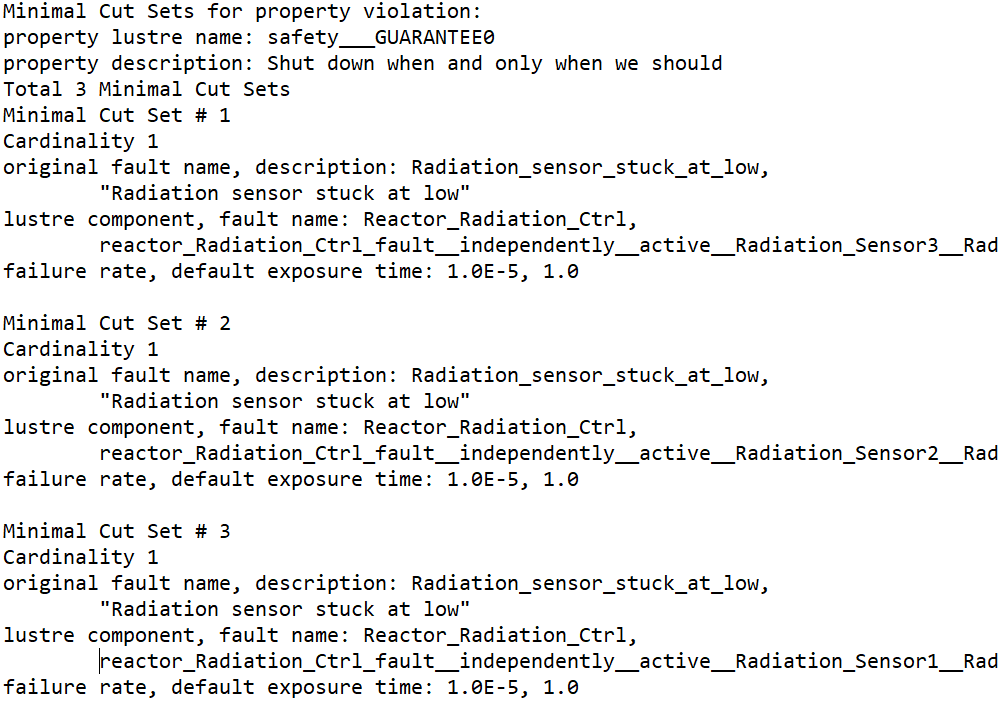
\includegraphics[scale=0.7]{images/detailedMCS.png}
	\caption{Detailed Output of MinCutSets}
		\label{fig:detailedMCS}
	\end{center}
\end{figure}

\item The minimal cut set information can be presented in tally form. This does not contain the fault information in detail, but instead gives only the tally of cut sets per property. This is useful in large models with many cut sets as it reduces the size of the text file. An example of this output type is seen in Figure~\ref{fig:tallyMCS}.
\begin{figure}[h!]
	\hspace*{-2cm}
	\vspace{-0.1in} 
	\begin{center}
		\includegraphics[scale=0.7]{images/TallyMCS.png}
	\caption{Tally Output of MinCutSets}
		\label{fig:tallyMCS}
	\end{center}
\end{figure}

\item The tool can also generate fault tree and minimal cut set information formatted as input to the SOTERIA tool~\cite{manolios2019model} to produce hierarchical fault trees that are consistent with the system architecture/component verification layers, or flat fault trees consist of minimal cut sets only, both in graphical form. A sample graphical fault tree output from the SOTERIA tool is shown in Figure~\ref{fig:soteriaFT}. The SOTERIA tool is also able to compute the probabilities for the top level event from a given fault tree. However, based on experience with the WBS example, our tool was a more scalable solution as it produces minimal cut sets for more complex systems, also in shorter amount of time. The text format of the minimal cut sets seemed anectodally easier to read than the graphical format for larger systems. 
% minimal cut set information can also be formatted as input to the SOTERIA tool \janet{[new soteria reference]} to display. 
%This
%\janet{The SOTERIA} tool can \janet{produce fault trees in }
%use the auto generated ocaml file to produce optimized fault trees in a graphical format instead of textual format. (See Section on SOTERIA for more information.) A sample output is shown in Figure~\ref{fig:soteriaMCS}. This \textit{.ml} file can be given as input to %SOTERIA to produce the optimized fault tree shown in Figure~\ref{fig:}. 
\begin{comment}
\begin{figure}[h!]
	\hspace*{-2cm}
	\vspace{-0.1in} 
	\begin{center}
		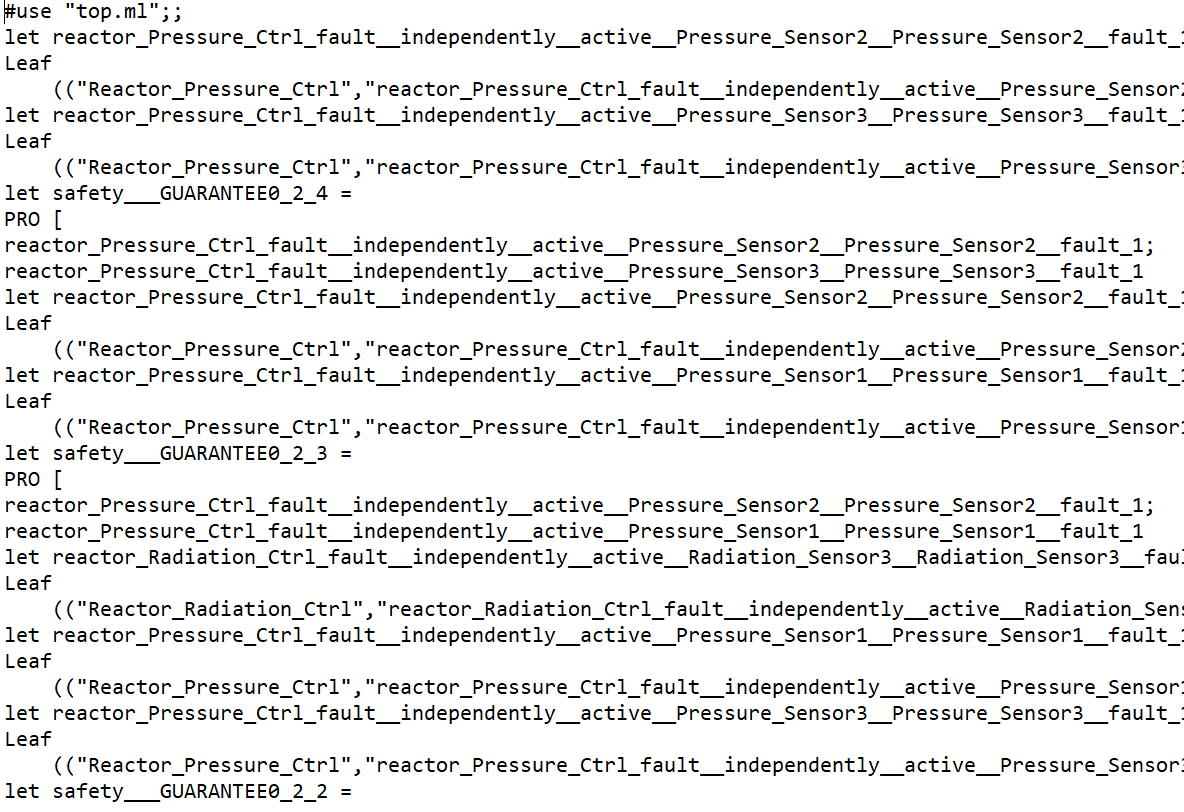
\includegraphics[scale=0.5]{images/soteriaMCS.png}
	\caption{SOTERIA Output of MinCutSets}
		\label{fig:soteriaMCS}
	\end{center}
\end{figure}
\end{comment}

\begin{figure}[h!]
	\hspace*{-2cm}
	\vspace{-0.1in} 
	\begin{center}
		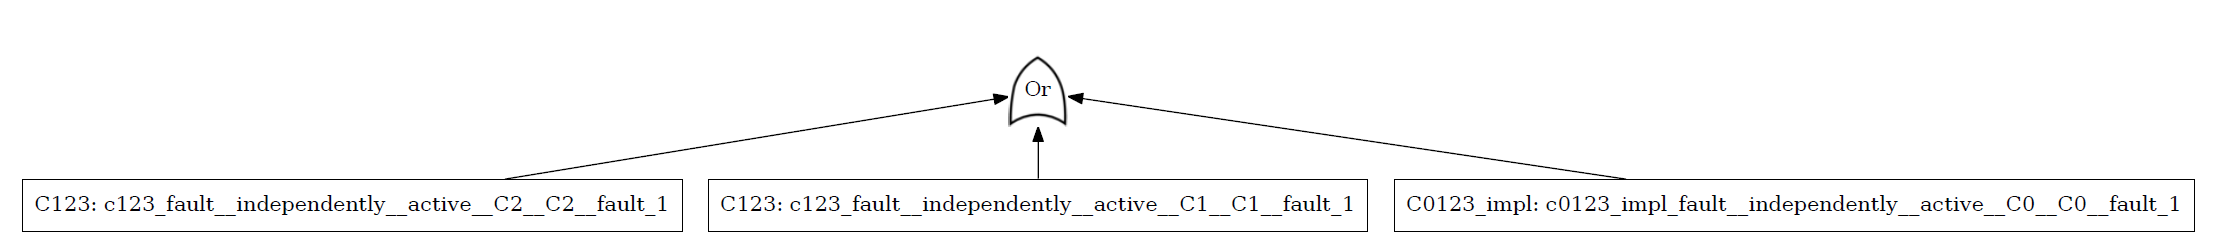
\includegraphics[scale=0.25]{images/Soteria_FT.png}
		\caption{Example SOTERIA Fault Tree}
		\label{fig:soteriaFT}
	\end{center}
\end{figure}

\end{enumerate}

\subsubsection{Use of Analysis Results to Drive Design Change}
We use a single top level requirement of the WBS: S18-WBS-0323 (Never indadvertent braking with all wheels locked to illustrate how Safety Annex can be used to detect design flaws and how faults can affect the behavior of the system). This safety property description can be found in detail in Section \ref{sec:fault_modeling}. Upon running max $n$ compositional fault analysis with $n = 1$, this particular fault was shown to be a single point of failure for this safety property. A counterexample is shown in Figure \ref{fig:counterexample} showing the active fault on the pedal sensor. 

\begin{figure}[h!]
	%\vspace{-0.2in}
	\begin{center}
		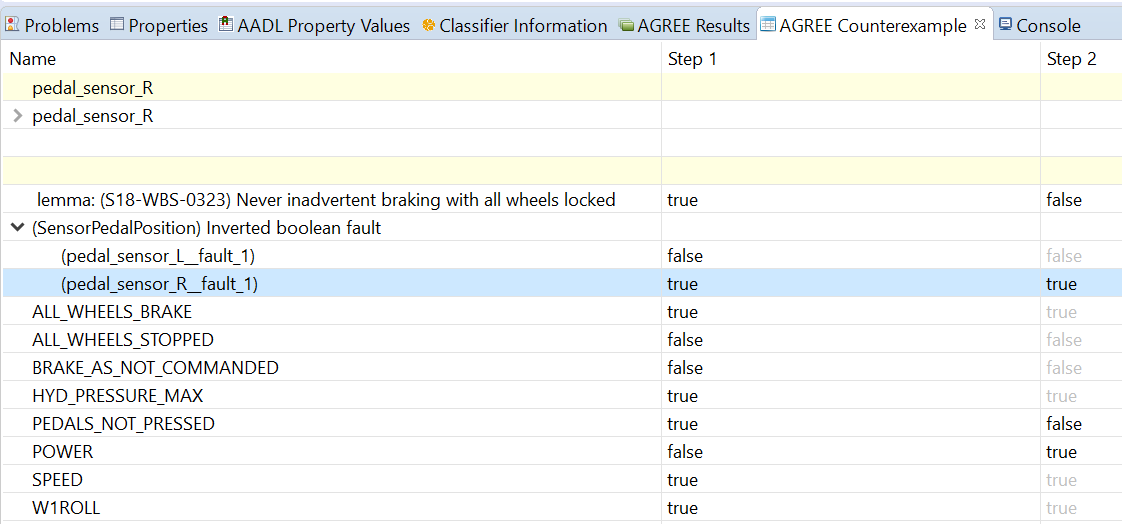
\includegraphics[width=\textwidth]{images/counterexample.png}
	\end{center}
	\vspace{-0.3in}
	\caption{AGREE counterexample for inadvertent braking safety property}
	\label{fig:counterexample}
	%\vspace{-0.2in}
\end{figure} 

Depending on the goals of the system, the architecture currently modeled, and the mitigation strategies that are desired, various strategies are possible to mitigate the problem.

\begin{itemize}
\item Possible mitigation strategy 1: Monitor system can be added for the sensor: A monitor sub-component can be modeled in which it accesses the mechanical pedal as well as the signal from the sensor. If the monitor finds discrepancies between these values, it can send an indication of invalid sensor value to the top level of the system. In terms of the modeling, this would require a change to the behavioral contracts which use the sensor value. This validity would be taken into account through the means of $valid \land pedal\_sensor\_value$. 
%In the real system however, this mitigation would need to be taken into account. Whether this is a flag to the pilot who can then override the electrical system and switch to a different mode or perform some other action to mitigate the failed sensor must be discussed and implemented. 

\item Possible mitigation strategy 2: Redundancy can be added to the sensor: A sensor subsystem can be modeled which contains 3 or more sensors. The overall output from the sensor system may utilize a voting scheme to determine validity of sensor reading. There are multiple voting schemes that are possible, one of which is a majority voting (e.g. one sensor fails, the other two take majority vote and the correct value is passed). 
When three sensors are present, this mitigates the single point of failure problem. New behavioral contracts are added to the sensor system to model the behavior of redundancy and voting. 
\end{itemize}

In the case of the pedal sensor in the WBS, the latter of the two strategies outlined above was implemented. A sensor system was added to the model which held three pedal sensors. The output of this subsystem was constrained using a majority voting scheme. Upon subsequent runs of the analysis (regardless which type of run was used), resilience was confirmed in the system regarding the failure of a single pedal sensor. Figure \ref{fig:sensorsystem} outlines these architectural changes that were made in the model.

\begin{figure}[h!]
	%\vspace{-0.2in}
	\begin{center}
		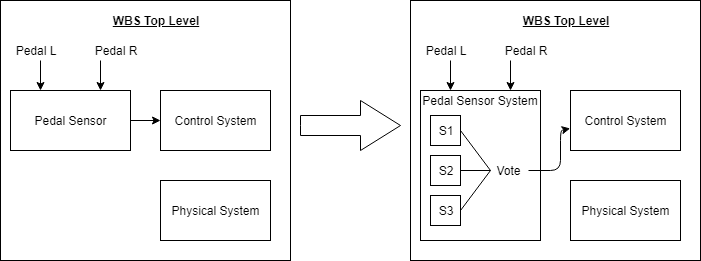
\includegraphics[width=\textwidth]{images/sensorsystem.png}
	\end{center}
	\vspace{-0.3in}
	\caption{Changes in the architectural model for fault mitigation}
	\label{fig:sensorsystem}
	%\vspace{-0.2in}
\end{figure}

As can be seen through this single example, a system as large as the WBS would benefit from many iterations of this process. Furthermore, if the model is changed even slightly on the system development side, it would automatically be seen from the safety analysis perspective and any negative outcomes would be shown upon subsequent analysis runs. This effectively eliminates any miscommunications between the system development and analysis teams and creates a new safeguard regarding model changes. 

For more information on types of fault models that can be created as well as details on analysis results, see the users guide located in the GitHub repository \cite{SAGithub}. This repository also contains all models used in this project. 




\section{Theoretical Foundations}
\label{sec:theory}
%As discussed in Section~\ref{sec:implementation}, there are two different types of analysis that can be performed on a fault model. The initial stages of the project implemented a \textit{Verify in the Presence of Faults} analysis that returned a single counterexample if a fault caused violation of a property. In later stages of this project, this was extended in order to collect all such fault combinations that caused these violations, \textit{Generate Minimal Cut Sets}. 

There are two different types of fault analysis that can be performed on a fault model, \textit{Verification in the Presence of Faults}, and \textit{Generate Minimal Cut Sets}, as introduced in Section~\ref{sec:implementation}. The theoretical foundations used to verify a model in the presence of faults relies on AGREE and the theory underlying the assume guarantee environment~\cite{cofer2012compositional}; this theory will not be discussed further in this report. The underlying theoretical framework used in the generation of minimal cut sets is described in detail in this section. 



%\subsection{Theory of Verification in the presence of Faults}
\label{sec:verify_theory}
The theoretical foundations used to verify a model in the presence of faults relies on AGREE and the theory used to prove the assume guarantee environment~\cite{cofer2012compositional}. 

\begin{comment}

Assuming that dependent faults have been collected and mapped appropriately, they are in the following form: \\
$\{\{f_1 \rightarrow\{f_3, f_7\}, f_5 \rightarrow\{f_2\},...\}$ meaning that $f_3$ and $f_7$ are dependent on $f_1$ and so on.

We make the assumption that there are no nested dependencies. To clarify this, we cannot have something of the form: \\
$f_1 \rightarrow \{f_3, f_5\}$\\
$f_3 \rightarrow \{f_4\}$

If this is the case, the user must define the dependency as follows: \\
$f_1 \rightarrow \{f_3, f_4, f_5\}$. 

\begin{algorithm}[H]
	% \KwData{this text}
	% \KwResult{how to write algorithm with \LaTeX2e }
	Input: $F$: map between allowable combination $F_i$ and associated probability (initially zero) \;
	Output: $F$: map between allowable combinations with dependencies and associated probability (nonzero) \;
	$newMCS =$ empty list \;
	$p=1$ \;
	\For{all allowable fault combinations $F_i \in F$}{
		Remove $F_i$ from $F$ \;
		\For{all $f_i \in MCS$ }{
		    \If{$f$ is key in dependency map}{
		    	$p = p*prob(f)$ \;
		    	append $f$ to $newMCS$ \;
		    	append dependent faults triggered by $f$ to $newMCS$ \;
		    	\For{all depFaults triggered by $f$ activation}{
		    		\If{depFault $\in MCS$}{
		    			remove depFault from $MCS$ \;
		    		}%end if depFault is in MCS
		    	} %end for all dep faults triggered
		    } %end if f is a key in the dependency map
		} % end for all faults in MCS
		Append $F_i \rightarrow p$ to $F$ \;
	}%end for all combos in F
	return $newMCS$ as the completed MCS \;
	\caption{Incorporate Dependencies}
	\label{alg:dep_alg}
\end{algorithm}

\end{comment}
%\subsection{Theory Behind the Generation of Minimal Cut Sets}
\label{sec:generate_theory}
The following sections describe in detail the background information, definitions, theory, and algorithms used in the process of generating minimal cut sets through the use of the All-MIVC algorithm.

\subsection{Fault Tree Analysis} 
The use of fault trees are common in many safety assessment processes and the ability to generate the cut sets needed for the construction of the fault tree is a useful part of any safety analysis tool. The fault tree is a safety artifact commonly referenced in requirement protocol documents such as ARP4761, ARP4754, and AIR6110~\cite{SAE:ARP4761,SAE:ARP4754A,AIR6110}.

% There are two main types of fault tree analysis that we differentiate here as \textit{qualitative} analysis and \textit{quantitative} analysis. In qualitative analysis, the structure of the fault tree is considered and the cut sets are a way to indicate which combinations of component failures will cause the system to fail. On the other hand, in quantitative analysis the probability of the TLE is calculated given the probability of occurance of the basic events. By being able to generate cut sets based on both probability and cardinality, this allows for either form of FTA to be created. 

A Fault Tree (FT) is a directed acyclic graph whose leaves model component failures and whose gates model failure propagation~\cite{0f356f05e72f43018211b36f97c8854a}. The system failure under examination is the root of the tree and is called the Top Level Event (TLE). The node types in a fault tree are \textit{events} and \textit{gates}. An event is an occurrence within the system, typically the failure of a subsystem down to an individual component. Events can be grouped into Basic Events (BEs), which occur independently, and \textit{intermediate events} which occur dependently and are caused by one or more other events~\cite{historyFTA}.  These events model the failure of the system (or subsystem) under consideration. The gates represent how failures propagate through the system and how failures in subsystems can cause system wide failures. The two main logic symbols used are the Boolean logic AND-gates and OR-gates. An AND-gate is used when the undesired top level event can only occur when all the lower conditions are true. The OR-gate is used when the undesired event can occur if any one or more of the next lower conditions is true. This is not a comprehensive list of gate types, but we focus our attention on these two common gate types. 
\begin{figure}[h]
\begin{center}
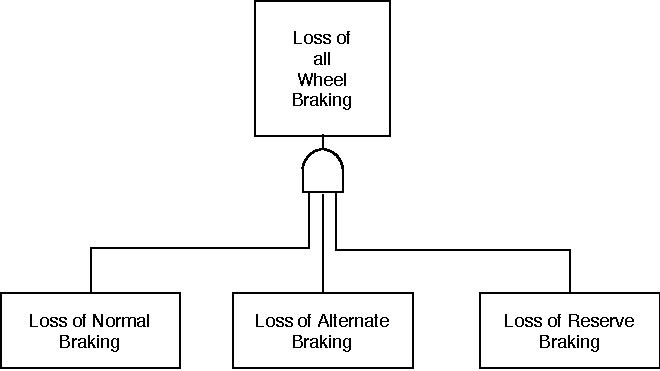
\includegraphics[width=8cm]{images/introFT2.pdf}
\caption{A simple fault tree} \label{fig:introFT}
\end{center}
\end{figure}

Figure~\ref{fig:introFT} shows a simple example of a fault tree based on SAE ARP4761~\cite{SAE:ARP4761}. In this example, the top level event corresponds to an aircraft losing all wheel braking. In order for this event to occur, all of the basic events must occur. This is seen through the use of the AND gate below the top level event. The gates in the fault tree describe how failures propagate through the system. Each gate has one output and one or more inputs. In Figure~\ref{fig:introFT}, the AND gate has three inputs and one output. The leaves of the tree represent the basic events of the system. %and 
In the case of this fault tree, these three events are also the Minimal Cut Sets (MinCutSets) for this top level event. A MinCutSet is the minimal set of basic events that must occur together in order to cause the TLE to occur. Generating and analyzing these MinCutSets is important to FTA and has been an active area of interest in the research community since fault trees were first described in Bell Labs in 1961~\cite{historyFTA,0f356f05e72f43018211b36f97c8854a}. 

There are two main types of fault tree analysis that we differentiate here as \textit{qualitative} analysis and \textit{quantitative} analysis. In qualitative analysis, the structure of the fault tree is considered and the MinCutSets are a way to indicate which combinations of component failures will cause the system to fail. On the other hand, in quantitative analysis the probability of the TLE is calculated given the probability of occurrence of the basic events. By being able to generate MinCutSets
based on both cardinality and probability, this allows for either form of FTA to be created. 


%\subsection{Inductive Validity Cores}

%Given a complex model, it is often useful to extract traceability information related to the proof, in other words, which portions of the model were necessary to construct the proof. An algorithm was introduced by Ghassabani, et. al. to provide Inductive Validity Cores (IVCs) as a way to determine which model elements are necessary for the inductive proofs of the safety properties for sequential systems~\cite{GhassabaniGW16}. Given a safety property of the system, a model checker can be invoked in order to construct a proof of the property. The IVC generation algorithm extracts traceability information from the proof process and returns a minimal set of the model elements required in order to prove the property. Later research extended this algorithm in order to produce all IVC elements~\cite{Ghassabani2017EfficientGO}. 

%The IVC algorithm considers a constraint system consisting of the assumptions and contracts of system components and the negation of the safety property of interest (i.e. the top level event). It then collects what are called Minimal Unsatisfiable Subsets (MUSs) of this constraint system; these are the minimal explanations of the constraint systems infeasibility in terms of the \textit{negation} of the safety property. Equivalently, these are the minimal model elements necessary to proof the safety property.

%In section \ref{sec:definitions}, we show the formal definitions of IVCs in detail. \\

%Our approach utilizes a few tools in order to generate the artifacts of interest and a brief background will be helpful. and hence the rest of the background section consists of a brief description of AADL, AGREE, and the SOTERIA tools and languages. 

%\subsection{Architecture Analysis and Design Language}
%We are using the Architectural Analysis and Design Language (AADL) to construct system architecture models.  AADL is an SAE International standard that defines a language and provides a unifying framework for describing the system architecture for ``performance-critical, embedded, real-time systems''~\cite{AADL_Standard,FeilerModelBasedEngineering2012}. From its conception, AADL has been designed for the design and construction of avionics systems.  Rather than being merely descriptive, AADL models can be made specific enough to support system-level code generation.  Thus, results from analyses conducted, including the new safety analysis proposed here, correspond to the system that will be built from the model.  

%An AADL model describes a system in terms of a hierarchy of components and their interconnections, where each component can either represent a logical entity (e.g., application software functions, data) or a physical entity (e.g., buses, processors). An AADL model can be extended with language annexes to provide a richer set of modeling elements for various system design and analysis needs (e.g., performance-related characteristics, configuration settings, dynamic behaviors). The language definition is sufficiently rigorous to support formal analysis tools that allow for early phase error/fault detection.

%\subsection{Compositional Analysis} Compositional analysis of systems was introduced in order to address the scalability of model checking large software systems. Monolithic verification and compositional verification are two ways that mathematical verification of component properties can be performed. In monolithic analysis, the model is flattened and the top level properties are proved using only the leaf level contracts of the components. On the other hand, the analysis can be performed compositionally following the architecture hierarchy such that analysis at a higher level is based on the components at the next lower level. The idea is to partition the formal analysis of a system architecture into verification tasks that correspond into the decomposition of the architecture. A component contract is an assume-guarantee pair. Intuitively, the meaning of a pair is: if the assumption is true, then the component will ensure that the guarantee is true. The components of a system are organized hierarchically and each layer of the architecture is viewed a system. For any given layer, the proof consists of demonstrating that the system guarantee is provable given the guarantees of its direct subcomponents and the system assumptions. This proof is performed one layer at a time starting from the top level of the system. When compared to monolithic analysis (i.e., analysis of the flattened model composed of all components), the compositional approach allows the analysis to scale to much larger systems~\cite{NFM2012:CoGaMiWhLaLu}. 

%\subsection{Assume Guarantee Reasoning Environment}
%The Assume Guarantee Reasoning Environment (AGREE) is a tool for formal analysis of behaviors in AADL models~\cite{NFM2012:CoGaMiWhLaLu}.  It is implemented as an AADL annex and annotates AADL components with formal behavioral contracts. Each component's contracts can include assumptions and guarantees about the component's inputs and outputs respectively, as well as predicates describing how the state of the component evolves over time.

%AGREE translates an AADL model and the behavioral contracts into Lustre~\cite{Halbwachs91:IEEE} and then queries a user-selected model checker to conduct the back-end analysis. The analysis can be performed compositionally or monolithically.

%\subsection{Safety Annex for AADL}
%The Safety Annex for AADL is a tool that provides the ability to reason about faults and faulty component behaviors in AADL models~\cite{Stewart17:IMBSA,SATechReport}. In the Safety Annex approach, formal assume-guarantee contracts are used to define the nominal behavior of system components. The nominal model is verified using AGREE. The Safety Annex weaves faults into the nominal model and analyzes the behavior of the system in the presence of faults. The tool supports behavioral specification of faults and their implicit propagation through behavioral relationships in the model as well as provides support to capture binding relationships between hardware and software compönents of the system. 

\begin{comment}
\subsection{SOTERIA}
The Safe and Optimal Techniques Enabling Recovery, Integrity, and Assurance (SOTERIA) tool is used to perform safety analysis of Integrated Modular Avionics (IMA) systems~\cite{SOTERIAproject}. In the SOTERIA project, a compositional modeling language was developed and this language is used as input in order to automatically synthesize the qualitative and quantitative safety analyses. The tool is compositional in that it requires safety aspects at each component level which enables the generation of compositional fault trees. 

\begin{figure}[h]
\begin{center}
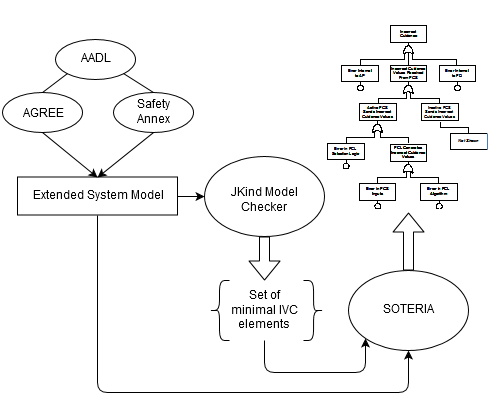
\includegraphics[width=8cm]{images/processFTA.png}
\caption{Outline of the fault tree generation process} \label{fig:processFTA}
\end{center}
\end{figure}

\end{comment}





\subsection{Definitions}
\label{sec:definitions}
Intuitively a constraint system contains the contracts that constrain component behavior and faults that are defined over these components. In the case of a nominal model augmented with faults, a constraint system is defined as follows. Let $F$ be the set of all fault activation literals defined in the model and $G$ be the set of all component contracts (guarantees). 

\begin{definition}A constraint system $C = \{C_1,C_2,...,C_n\}$ where for $i \in \{1,...,n\}$, $C_i$ has the following constraints for any $f_j \in F$ and $g_k \in G$ with regard to the top level property $P$: 
\begin{center}
$C_i \in \left\{ \begin{array}{ll}
	f_j :&  inactive\\
	g_k :& true\\
	P :& false\\
\end{array}\right.$	
\end{center}
\label{def:constraintsystem}
\end{definition}

Given a state space $S$, a transition system $(I,T)$ consists of the initial state predicate $I : S \rightarrow \{0,1\}$ and a transition step predicate $T : S \times S \rightarrow \{0,1\}$. Reachability for $(I,T)$ is defined as the smallest predicate $R : S \rightarrow \{0,1\}$ that satisfies the following formulas:
\begin{center}
$\forall s. I(s) \Rightarrow R(s)$\\
$\forall s, s' .  R \land T(s,s') \Rightarrow R(s')$\\
\end{center}
A safety property $\mathcal{P} : S \to \{0,1\}$ is a state predicate. A safety property $\mathcal{P}$ holds on a transition system $(I,T)$ if it holds on all reachable states. More formally, $\forall s . R(s) \Rightarrow \mathcal{P}(s)$. When this is the case, we write $(I,T) \vdash\mathcal{P}$~\cite{Ghassabani2017EfficientGO}. 

Given a transition system that satisfies a safety property $P$, it is possible to find which model elements are necessary for satisfying the safety property through the use of the \textit{All Minimal Inductive Validity Cores All-MIVCs} algorithms~\cite{Ghassabani2017EfficientGO,bendik2018online}. This algorithm collects all minimal unsatisfiable subsets of a given transition system in terms of the negation of the top level property. The minimal unsatisfiable subsets consist of component contracts constrained to \textit{true}. When the constraints on these model elements are removed from the constraint system $C$, this results in an UNSAT system. This can be seen as the minimal explanation of the constraint systems infeasibility. Recall that this constraint system is in terms of the \textit{negation} of the safety property. Thus, this algorithm provides all model elements required for the proof of the safety property. 

We utilize this algorithm by providing not only component contracts (constrained to \textit{true}) as model elements, but also fault activation literals constrained to \textit{false}. Thus the resulting MIVCs will contain the required contracts and constrained fault activation literals in order to prove the safety property. This information is used throughout this section to provide the underlying theory behind the generation of minimal cut sets from all MIVCs. 

Definitions 1-3 are taken from research by Liffiton et. al.~\cite{liffiton2016fast}. 

\begin{definition} : A Minimal Unsatisfiable Subset ($MUS$) of a constraint system $C$ is :\\
 $\{MUS \subseteq C$ $|$ $MUS$ is UNSAT and $\forall c \in MUS$: $MUS \setminus \{c\}$ is SAT$\}$. This is the minimal explaination of the constraint systems infeasability. 
\end{definition}

A closely related set is a \textit{minimal correction set} (MCS). The MCSs describe the minimal set of model elements for which if constraints are removed, the constraint system is satisfied. For constraint system $C$, this corresponds to which faults are not constrained to inactive (and are hence active) and violated contracts which lead to the violation of the safety property. In other words, the minimal set of active faults and/or violated properties that lead to the top level event.  

\begin{definition} : A Minimal Correction Set ($MCS$) of a constraint system $C$ is :\\
 $\{MCS \subseteq C$ $|$ $C \setminus MCS$ is SAT and $\forall S \subset MCS$ : $C \setminus S$ is UNSAT$\}$. A MCS can be seen to ``correct'' the infeasability of the constraint system.
\end{definition}

A duality exists between MUSs of a constraint system and MCSs as established by Reiter \cite{reiter1987theory}. This duality is defined in terms of \textit{minimal hitting sets}. A hitting set of a collection of sets $A$ is a set $H$ such that every set in $A$ is ``hit'' be $H$; $H$ contains at least one element from every set in $A$ \cite{liffiton2016fast}. The MCSs can be generated from the MUSs if all MUSs are known. Thus, the use of the All-MIVCs algorithm is required. 

\begin{definition}: Given a collection of sets $K$, a hitting set for $K$ is a set $H \subseteq \cup_{S \in K} S$ such that $H \cap S \neq \emptyset$ for each $S  \in K$. A hitting set for $K$ is minimal if and only if no proper subset of it is a hitting set for $K$. 
\end{definition}

Utilizing this approach, the MCSs are generated from the MUSs that are provided by the All-MIVCs algorithm~\cite{Ghassabani2017EfficientGO} and a minimal hitting set algorithm developed by Murakami et. al.~\cite{murakami2013efficient,gainer2017minimal}. \\

A Minimal Cut Set ($MinCutSet$) is a minimal collection of faults that lead to the violation of the safety property (or in other words, lead to the top level event in the fault tree). We define a minimal cut set consistently with much of the research in this field~\cite{0f356f05e72f43018211b36f97c8854a,historyFTA}

\begin{definition} :  A Minimal Cut Set can be defined as the set of faults in a system that cause the violation of the safety property. Furthermore, any strict subset of these faults will not cause violation of the safety property. 
\end{definition}








\subsection{Transformation of All-MIVCs into Minimal Cut Sets}
\label{sec:transformation}
%The IVCs
All Minimal Inductive Validity Cores are collected by use of the All-MIVCs algorithm~\cite{Ghassabani2017EfficientGO}. These are all of the Minimal Unsatisfiable Subsets (MUSs) which can be used as input to the Minimal Hitting Set algorithm~\cite{murakami2013efficient,gainer2017minimal} in order to collect all Minimal Correction Sets (MCSs). The MCSs are then transformed into Minimal Cut Sets according to the following theoretical results. 

The definition of the constraint system follows Definition 1 in Section~\ref{sec:definitions}.

\begin{theorem}  The MinCutSet can be generated by the transformation of the Minimal Correction Set (MCS).

\begin{proof}  All $MCS$s are of the form $MCS = G \cup \overline{F}$ where $G$ consists of contracts in the system and $\overline{F}$ consists of faults constrained to false for constraint system $C$. 

\textbf{Case 1}: $G = \emptyset$\\
In the leaf level of the system, only constrained faults are contained in $MCS$. According to the defintion of an $MCS$, upon removing the constraints from $C$ of the elements contained in the $MCS$, the constraint system is satisfiable. Furthermore, the $MCS$ is the minimal such set. Thus, the constraint system with the \textit{active} faults from $MCS$ will cause the \textit{negation} of the safety property to be satisfied. The set of unconstrained faults found in the $MCS$ is the defintion of a minimal cut set. 

\textbf{Case 2}: $G \neq \emptyset$\\
Let $MCS = \{\lnot f_1,...,\lnot f_n,g_1,...,g_m\}$ where $f_j \in F$ and $g_k \in G$ and $\lnot f$ is a fault activation literal $f$ constrained to \textit{false}. 
For all $g_i \in MCS$, we know that the validity of $g_k$ is required in the proof of the top level property $P$ due to its generation through the All-MIVCs algorithm. For $g_1 \in MCS$, there exists a set containing all minimal cut sets of $g_1$. Call this $Cut(g_1) = \{F_{1i} \subseteq F | F_{1i}$ is a min cut set for $g_1, i = 1,...,p_1\}$. 

Replace $g_1$ with $F_{1i}$ for all $i = 1,...,p_1$. This produces $p_1$ new MCSs of the form:
\begin{center}
$\{f_1,...,f_n,F_{11},...,g_m\}$\\
$\{f_1,...,f_n,F_{12},...,g_m\}$\\
$\vdots$\\
$\{f_1,...,f_n,F_{1p_1},...,g_m\}$\\
\end{center}

Perform this replacement for all $g_k \in MCS$, $k=1,...,m$. %This produces at most $|p_1| \times \hdots \times |p_m|$ MCSs containing only faults. 

Let $I_\alpha$ be one of the sets generated by full replacement of all contracts in some $MCS_\alpha$ with their respective minimal cut set and all fault activation literals constrainted to \textit{true}.\\

\textit{Claim: $I_\alpha$ is a minimal cut set for safety property $P$}\\
By the definition of $MCS_\alpha$, $C\setminus MCS_\alpha$ is SAT. Thus the fault activation literals in $MCS_\alpha$ are \textit{true} and the contracts in $MCS_\alpha$ are violated. This combination will cause violation of the safety property (i.e., the constraint system $C\setminus MCS_\alpha$ is SAT). 

The generation of $I_\alpha$ consists of replacing all contracts in $MCS_\alpha$ by their respective minimal cut sets and unconstraining all fault activation literals in $MCS_\alpha$. These unconstrained faults cause the violation of all contracts in $MCS_\alpha$. Hence together, the violation of $P$ since $C\setminus MCS_\alpha$ is SAT. Therefore $I_\alpha$ is a cut set for $P$.\\

Minimality follows from the defintion of $MCS$: \\

Assume that $I_\beta \subset I_\alpha$. Then there is at least one $f \in I_\alpha$ where $f \not \in I_\beta$. Let $\lnot f$ be the fault activation literal $f$ constrained to \textit{false}. \\

If $ \lnot f \in MCS_\alpha$ and $f \not \in I_\beta$, then by removing all constraints of the fault literals in $I_\beta$ from $C$ ($C \setminus I_\beta$), we see that the resulting constraint system is UNSAT by the minimality of $MCS_\alpha$. Therefore $I_\beta$ is not a cut set for $P$.\\

If $f \in MinCut(g)$ where $MinCut(g)$ is a minimal cut set for some $g \in MCS_\alpha$, then $C \setminus I_\beta$ will not remove constraints for all of the elements in $MinCut(g)$ and therefore $g$ remains unviolated, i.e., the constraint that $g$ is \textit{true} is not removed. Thus $C \setminus I_\beta$ will not remove constraints for all of the elements in $MCS_\alpha$ which means $C \setminus I_\beta$ is UNSAT. Therefore $I_\beta$ is not a cut set for $P$.

\end{proof}
\end{theorem}

The generation of MIVCs traverses the program in a top down fashion. The transformation of MIVCs to MinCutSets traverses this tree in a bottom up fashion if and only if All-MIVCs have been generated. It is a requirement of the minimal hitting set algorithm that \textit{all} MUSs are used to find the MCSs~\cite{liffiton2016fast,gainer2017minimal,murakami2013efficient}. Thus, once All-MIVCs have been found and the minimal hitting set algorithm has completed, %our 
the MinCutSets Generation algorithm can begin. 

%Initially, we begin with a list of MCSs for each layer. As mentioned previously, at the leaf layer this set only contains constrained faults, but at intermediate layers it is possible for the MCSs to contain a mixture of both constrained inactive faults and valid contracts. When this is the case, a replacement must be made between the contracts and the faults in the model that can cause their violation. Once this replacement begins, this set is no longer an MCS nor is it yet a MinCutSet. We call this set $I$ for \textit{Intermediate Set} in the following algorithm. 

%Initially, we begin
The MinCutSets Generation Algorithm begins with a list of $MCSs$ specific to a top level property. These $MCSs$ may contain a mixture of fault activation literals constrained to \textit{false} and %\textit{true} subcomponent contracts.
and subcomponent contracts constrained to \textit{true}. We remove all constraints from each $MCS$ and call the resulting sets $I$, for \textit{Intermediate} set. Replacement of subcomponent contracts with their respective minimal cut sets can then proceed. For each of those contracts in $I$, we check to see if we have previously obtained a $MinCutSet$ for that contract. If so, replacement is performed. If not, we recursively call this algorithm to obtain the list of all %$MCSs$ 
MinCutSets associated with this subcomponent contract. At a certain point, there will be no more contracts in the set $I$ in which case we have a minimal cut set for the current property. When this set is obtained, we store it in a lookup table keyed by the given property that this $I$ is associated with. 

%Initially, we begin with a list of MCSs for each layers contracts. At the leaf layer, the MCSs only contain constrained to inactive faults, and we remove the constraints to obtain MinCutSet for each component contract at the leaf layer. At the intermediate layers, the MCSs can contain a mixture of constrained inactive faults and valid component contracts. We first remove the constraints on them to obtain an \textit{Intermediate Set}, $I$, that contains active faults and invalid subcomponent contracts, and replace each invalid subcomponent contract with the MinCutSet obtained for that contract from the layer below. We call this intermediate set $I$ in the following algorithm and $List(I)$ is the set of all $MCSs$ for a component contract at the start of the algorithm and all intermediate sets once replacement begins. At the end of the algorithm the minimal cut sets for the top level property are generated.

Notes regarding the following algorithm: at the onset, the current property $P$ is a top level property. Each of the properties has a list of associated $MCSs$. When the algorithm states that constraints on these elements are removed, more specifically the fault activation literals in $MCS$ are constrained to \textit{true} and the component contracts are constrained to \textit{false}. $List(I)$ is the collection of all $MCSs$ with all constraints removed. Assuming All-MIVCs have been found and the minimal hitting set algorithm has terminated, giving us a list of $MCSs$ for each property in the system. 


\begin{algorithm}[H]
\SetKwFunction{FMain}{replace}
 \SetKwProg{Fn}{Function}{:}{}

	\Fn{\FMain{$P$}}{
		$List(I)$:= $List(MCS)$ for $P$ with all constraints removed \;
		\For{all $I \in List(I)$}{
			\eIf{there exists constrained contracts $g \in I$}{
				\For{all constrained contracts $g \in I$}{
					\eIf{there exists $MinCutSets$ for $g$ in lookup table}{
						\For{all $minCut(g)$}{
							$I_{repl} = I$ \;
							$I_{repl} :=$ replace constrained $g$ with $minCut(g)$ \;
							add $I_{repl}$ to $List(I)$ \;
						} %end for all cut sets of g
					}{
						replace($g$) \;
					} % end else if no cut sets in lookup table
				} % end for all constrained contracts in I
			}{
				add $I$ as $minCut(g)$ for $P$ \;
			} %end else if there exists contracts in I
		}%end for all I in list(I)
	}
%	\caption{Minimal Cut Set Generation Algorithm}
	\caption{MinCutSets Generation Algorithm}
	\label{alg:generation_alg}
\end{algorithm}

The number of replacements $R$ that are made in this algorithm are constrained by the number of minimal cut sets there are 
for all $\alpha$ contracts within the set \textit{I}. %$MCS$. 
We call the set of all minimal cut sets for a contract $g$: $Cut(g)$. The following formula defines an upper bound on the number of replacements. The validity of this statement follows directly from the general multiplicative combinatorial principle. Therefore, the number of replacements $R$ is bounded by the following formula where $g_1$ is the first contract being processed in the set \textit{I}.

$R \leq |Cut(g_1)| +  {\displaystyle \sum_{i=1}^{\alpha} }({\displaystyle \prod_{j=1}^{i} |Cut(g_j)|})$\\ 

It is also important to note that the cardinality of $List(I)$ is bounded, i.e. the algorithm terminates. Every new $I$ that is generated through some replacement of a contract with its minimal cut set is added to $List(I)$ in order to continue the replacement process for all contracts in $I$. Thus, the same bound for the number of replacements exists for the size of $List(I)$. Since no infinite sets (either MIVCs or MCSs) are generated by the All-MIVC or minimal hitting set algorithms, all sets are finite.

The reason for this upper bound is that for a contract $g_1$ in $MCS$, we make $|Cut(g_1)|$ replacements and add the resulting lists to $List(I)$. Then we move to the next contract $g_2$ in $I$. We must additionally make $|Cut(g_1)| \times |Cut(g_2)|$ replacements and add all of these resulting lists to $List(I)$, and so on throughout all contracts. Through the use of basic combinatorial principles, we end with the above formula for the upper bound on the number of replacements. 

%%%%%%%%%%%%%%%%%%%%%%%%%%%%%%%%%%%%%%%%%%%%

The results from this algorithm are the minimal cut sets for the top level properties. These are presented to the user as described in Section~\ref{sec:fault_analysis_2}.

The MinCutSets are filtered during this process based on the fault hypothesis given. Algorithm~\ref{alg:generation_alg} is the general approach, but this changes slightly depending on which form of analysis is being performed. These differences are outlined in the following subsections.



































\subsubsection{Transformation Algorithm for Max N Analysis}
Given a top level fault hypothesis statement of maximum $N$ faults, the transformation algorithm filters out any MinCutSets of cardinality greater than $N$. To assist in performance and scalability, if a minimum cut set exceeds the cardinality of $N$, it will no longer be considered for the algorithm. We call this \textit{pruning}. This pruning is done in Algorithm 2 in Section~\ref{sec:transformation}. If the number of faults in an intermediate set $I$ exceeds $N$, any further replacement of remaining contracts in that intermediate set can never decrease the total number of faults in $I$. Only the remaining sets are displayed. 











































\subsubsection{Probabilistic Analysis Algorithm}
\label{sec:probAlg}
In order to complete the probabilistic analysis, we must first calculate allowable combinations of faults. This allows us the option to eliminate unnecessary combinations while performing the algorithm, thus increasing performance and diminishing the problem of combinatorial explosions in the size of minimal cut sets for larger models. 

After the allowable combinations have been found, the algorithm described in Section~\ref{sec:transformation} is performed with pruning in order to eliminate probabilistically impossible fault combinations. \\

\textbf{Collect Allowable Fault Combinations}
The collection of allowable fault combinations is a prerequsite needed for both \textit{Verify in the Presence of Faults} and \textit{Generate Minimal Cut Set} analysis and the algorithm used is described in Section 6.2.2.  In order to calculate allowable combinations, we must take into account probabilities of the combined faults and compare with the given threshold. Each of the allowable fault combinations has a combined probability that we must later access. These combinations are saved in a list called $\mathcal{A}$:

$\mathcal{A} = \{A_i = FaultCombinations$ $|$  $P(FaultCombinations) > threshold\}$

The allowable combinations in $\mathcal{A}$ consist of independent faults. \\


%\textbf{Generate Minimal Cut Sets and Prune Combinations}
\textbf{Prune MinCutSets}
During the transformation process, if the minimal cut set for a contract is not a subset of any allowed fault combinations, this intermediate set containing this contract is pruned. (Recall that an intermediate set $I$ is obtained by removing all constraints from an $MCS$ and contract replacement has begun.) This pruning occurs in the algorithm described in Section~\ref{sec:transformation} and the resulting allowable combinations are displayed to the user.

%Theoretically, there are other places that pruning can occur in this algorithm. The implementation of the Safety Annex utilizes the pruning as described previously. Throughout this discussion, we use the following notation to describe these sets. They are listed here for convenience. 

The implementation of the Safety Annex utilizes the pruning as described above. Theoretically, there are two other options for pruning in this algorithm. They are outlined here for completion. Throughout this discussion, we use the following notation to describe these sets. They are listed here for convenience.

$\mathcal{A}$ : the set of all allowable fault combinations 

$\mathcal{A}_i $ : an individual allowable combination and an element of $\mathcal{A}$

$List(I)$ : the set of all intermediate sets

$I_i$ : an element of $List(I)$. 

$Cut(g_j)$ : all minimal cut sets for contract $g_j$. 

$cut_k(g_j)$ : a specific cut set for contract $g_j$. This is an element of $Cut(g_j)$.  \\

\textbf{Option 1}: Once the replacement is complete and the algorithm terminates, we have all $MinCutSets$ for a top level property. If $MinCutSet \not \subseteq \mathcal{A}_i$ for all $\mathcal{A}_i \in \mathcal{A}$, then we can safely eliminate $MinCutSet$. This is the latest form of pruning and the drawback is when the number of generated cut sets grows, no elimination occurs early. This can be difficult in terms of scalability. 

\textbf{Option 2}: Pruning can also be done by checking the union of a minimal cut set for a contract in $I$ with all the faults in that $I$. If the union of these faults is not an allowable combination, %it can be eliminated.
the minimal cut set for this contract in $I$ will be skipped for the replacement. More formally, if ($\{f_n | f_n \in I_i\} \cup cut_k(g_j)) \not \subseteq  \mathcal{A}_i $ for all $\mathcal{A}_i \in \mathcal{A}$, then we can safely eliminate this $I_i$. 

































\begin{comment}
At the leaf level, only faults are contained in IVCs (and consequently in $MCS$s). Thus we store these cut sets in a lookup table for quick access throughout the algorithm. For this algorithm, we assume we are in an intermediate level of the analysis. Given a hypothesis probability threshold, we find only the cut sets that contain allowable combinations of faults in terms of probability of occurrance. Assume we have used the hitting set algorithm to generate $MCS$s from the IVCs and we have calculated allowable fault combinations. This is where the algorithm begins. \\

Throughout this discussion, we use the following notation to describe these sets. They are listed here for convenience. 

$List(MCS)$ : the set of all MCSs

$MCS_i$ : an element of $List(MCS)$. 

$Cut(g_j)$ : all minimal cut sets for contract $g_j$. 

$cut_k(g_j)$ : a specific cut set for contract $g_j$. This is an element of $Cut(g_j)$.  \\

In this algorithm, we have a few options where to prune sets that do not correspond with allowed combinations. For completion, we include a discussion on these three options. In our implementation, we chose to perform Option 1 and pruned after inlining was complete. 

\textbf{Option 1}: Once the inlining is complete and we have a minimal cut set, if $MinCutSet \not \subseteq \mathcal{F}_i $, then we can safely eliminate $MinCutSet$. We avoid the overhead of checking subsets in $\mathcal{F}$, but we have the complete overhead of inlining. 

\textbf{Option 2}: Pruning can also be done to a $MCS$ if the cut set for any contract within a $MCS$ is not an allowable combination. More formally, if $cut_k(g_j) \not \subseteq \mathcal{F}_i$ where $\mathcal{F}$ is the set of all possible combinations $\mathcal{F}_i $, then we can safely eliminate the $MCS_i$ in which $g_j$ is located. This option has benefits terms of early elimination, but would have a detrimental overhead in other areas. A search over $\mathcal{F}$ is required to determine if $cut_k(g_j)$ is a subset of one of the allowed combinations and a final elimination after inlining is complete would also be required.

%Ex: Let $\mathcal{F} = \{\{f_1,f_2,f_5\},\{f_6\}\}\}$ be the allowed fault combinations. Let $MCS = \{f_1,g_1,g_2\}$,  $Cut(g_1) = \{\{f_2\}\}$, $Cut(g_2) = \{\{f_5\},\{f_6\}\}$. Then for option 2, we would not eliminate anything: $cut_1(g_1) = \{f2\} \subseteq \mathcal{F}_i$ and likewise for $cut_1(g_2)$ and $cut_2(g_2)$. 

%The MCSs generated through the inlining process are: $MCS_1 = \{f_1,f_2,f_5\}$ and $MCS_2 = \{f_1,f_2,f_6\}$ which provides one combination which should be eliminated. Thus we would have to perform another check at the end of the algorithm to eliminate these. \\

\textbf{Option 3}: Pruning can also be done by checking the union of a cut set for a contract in $MCS$ with the faults in that $MCS$. If the union of these faults is not an allowable combination, it can be eliminated. More formally, if ($\{f_n | f_n \in MCS_i\} \cup cut_k(g_j)) \not \subseteq  \mathcal{F}_i $, then we can safely eliminate this $MCS_i$.This option is beneficial in that we do not have to perform two searches in $\mathcal{F}$, but has the drawback of needing to find the union of all faults located in $MCS_i$, ignoring the $g_j$ in $MCS_i$, and then performing the subset search through $\mathcal{F}$. 


%Upside: $List(MCS)$ does not grow as fast IF we can eliminate things along the way.\\

%Downside: Worst case scenario, every $cut_k(g_j)$ has to be combined with faults in $MCS_i$ and a complete search of all subsets of $\mathcal{F}$ completed for every $MCS_i$ and NOTHING is eliminated. In this scenario, it is more efficient to wait until the end and do one search through $\mathcal{F}$ and eliminate accordingly. \\

%Let $|MCS| = n$ ($MCS = \{MCS_1,...,MCS_n\}$). In the worst case scenario, we have a contract in every $MCS_i$. There are $\alpha_i$ contracts in $MCS_i$. 

%Every contract has $m_{g_\alpha}$ minimal cut sets. Then every cut set is combined with faults remaining in $MCS_i$ and searched for in $\mathcal{F}_i$. \\ 



%Which option is better? For now in the algorithm, I will just write Option 1, Option 2, Option 3 in their respective locations. This assumes that if option 1 is used, options 2 and 3 are removed from the algorithm. Obviously. The choice of option will also change a lot depending on our data structures for these lists and what algorithms we use to check for subsets within lists. It is also highly dependent on the model that is used in this analysis. Depending on the model itself, different options would be more efficient.

\begin{algorithm}[H]
	% \KwData{this text}
	% \KwResult{how to write algorithm with \LaTeX2e }
	Input 1: $List(MCS)$ : MCSs that contain contracts \;
	Input 2: $Cut(g_j)$ : all minimal cut sets of the contract $g_j$ \;
	Output: List of allowed minimal cut sets \;
	$P_{List} = \{\}$ List that will hold the probabilities associated with each allowed $MinCutSet$ generated \;
	%$0 < j \leq \alpha$ \;
	%$0 < i \leq \gamma$ \;
	\For{all $MCS_i \in List(MCS)$ }{
	    Remove $MCS_i$ from $List(MCS)$\;
	    \For{all $g_j\in MCS_i$}{
		Remove $g_j$ from $MCS_i$ \;
		\For{all $cut_k(g_j) \in Cut(g_j)$}{
			\textbf{Option 2} : if $cut_k(g_j) \subseteq \mathcal{F}_i $ for some $\mathcal{F}_i  \in \mathcal{F}$, then add $cut_k(g_j)$ to $MCS_i$ else break \; 
			\textbf{Option 3}: if union of faults in $MCS_i$ with $cut_k(g_j)$ is subset of $\mathcal{F}_i $
				     for some $\mathcal{F}_i \in \mathcal{F}$, then add $cut_k(g_j)$ to $MCS_i$ else break \;
			\eIf{$\exists g\in MCS_i$}{
				Add $MCS_i$ to $List(MCS)$ \;
			}{
				
				\textbf{Option 1 and 2}: if $MCS_i \in \mathcal{F}$, add dependencies, calculate probability, and append $p(MCS_i)$ to $P_{List}$ , else break \;
				\textbf{Option 3} : add dependencies, calculate probability, and append $p(MCS_i)$ to $P_{List}$ \;
				
			}%end if-else there is another contract in MCS
		} % end for cut_i(g)
               } % end for contracts in MCS_i
	} % end for List(MCS)
	Overall probability $= sum\{p_i \in P_{List}\}$ \;
	\caption{Minimal Cut Set Generation for Probabilistic Analysis}
	\label{alg:prob_alg}
\end{algorithm}








\textbf{Step 3: Incorporate Dependencies and Calculate Probability}
\janet{Make step 3 of incorporating dependencies another subsection of 7.3, and remove "calculate probability"}
Assuming that dependent faults have been collected and mapped appropriately, they are in the following form: \\
$\{\{f_1 \rightarrow\{f_3, f_7\}, f_5 \rightarrow\{f_2\},...\}$ meaning that $f_3$ and $f_7$ are dependent on $f_1$ and so on.

We make the assumption that there are no nested dependencies. To clarify this, we cannot have something of the form: \\
$f_1 \rightarrow \{f_3, f_5\}$\\
$f_3 \rightarrow \{f_4\}$

If this is the case, the user must define the dependency as follows: \\
$f_1 \rightarrow \{f_3, f_4, f_5\}$. 

\begin{algorithm}[H]
	% \KwData{this text}
	% \KwResult{how to write algorithm with \LaTeX2e }
	Input: $F$: map between allowable combination $F_i$ and associated probability (initially zero) \;
	Output: $F$: map between allowable combinations with dependencies and associated probability (nonzero) \;
	$newMCS =$ empty list \;
	$p=1$ \;
	\For{all allowable fault combinations $F_i \in F$}{
		Remove $F_i$ from $F$ \;
		\For{all $f_i \in MCS$ }{
		    \If{$f$ is key in dependency map}{
		    	$p = p*prob(f)$ \;
		    	append $f$ to $newMCS$ \;
		    	append dependent faults triggered by $f$ to $newMCS$ \;
		    	\For{all depFaults triggered by $f$ activation}{
		    		\If{depFault $\in MCS$}{
		    			remove depFault from $MCS$ \;
		    		}%end if depFault is in MCS
		    	} %end for all dep faults triggered
		    } %end if f is a key in the dependency map
		} % end for all faults in MCS
		Append $F_i \rightarrow p$ to $F$ \;
	}%end for all combos in F
	return $newMCS$ as the completed MCS \;
	\caption{Incorporate Dependencies}
	\label{alg:dep_alg}
\end{algorithm}

The results from this algorithm are all minimal cut sets with combined probability greater than or equal to the threshold given at the top level. \\


\end{comment}














































































\section{Related Work}
\label{sec:related_work}

A model-based approach for safety analysis was proposed by Joshi et. al in \cite{Joshi05:Dasc, Joshi05:SafeComp, Joshi07:Hase}.  In this approach, a safety analysis system model (SASM) is the central artifact in the safety analysis process, and traditional safety analysis artifacts, such as fault trees, are automatically generated by tools that analyze the SASM.

The contents and structure of the SASM differ significantly across different conceptions of MBSA.  We can draw distinctions between approaches along several different axes.  The first is whether they propagate faults explicitly through user-defined propagations, which we call {\em failure logic modeling} (FLM) or through existing behavioral modeling, which we call {\em failure effect modeling} (FEM).  The next is whether models and notations are {\em purpose-built} for safety analysis vs. those that extend {\em existing system models} (ESM).

For FEM approaches, there are several additional dimensions.  One dimension involves whether {\em causal} or {\em non-causal} models are allowed.  Non-causal models allow simultaneous (in time) bi-directional %failure
error propagations, which allow more natural expression of some failure types (e.g. reverse flow within segments of a pipe), but are more difficult to analyze.  A final dimension involves whether analysis is {\em compositional} across layers of hierarchically-composed systems or {\em monolithic}.  Our approach is an extension of AADL (ESM), causal, compositional, mixed FLM/FEM approach.

%We believe this is in a unique area of the trade space compared to other state-of-the-art MBSA approaches.

%Formal model based systems engineering (MBSE) methods and tools now permit system level requirements to be specified and analyzed early in the development process~\cite{QFCS15:backes,CIMATTI2015333, NFM2012:CoGaMiWhLaLu, hilt2013:MuWhRaHe}. Design models from which aircraft systems are developed can be integrated into the safety analysis process to help guarantee accurate and consistent results. Integration of MBSA into safety analysis process is described by Bozzano and Villafiorita~\cite{Bozzano:2010:DSA:1951720}. There are tools that currently support reasoning about faults in architecture description languages such as SysML and AADL. We provide here a brief overview of the most relevant safety analysis tools.

%In analyzing an EMV2 model of the WBS, we found missing feedback loops between the wheels and BSCU
%Interactions are easily overlooked by analysts and thus not explicitly described. In our approach, faults are injected into the system and behaviorally propagated through the use of assume-guarantee statements in AGREE. This avoids the difficulties inherent with explicit fault enumeration and propagation.

Tools such as the AADL Error Model Annex, Version 2 (EMV2)~\cite{EMV2} and HiP-HOPS for EAST-ADL~\cite{CHEN201391} are {\em FLM}-based {\em ESM} approaches.  As previously discussed, given many possible faults, these propagation relationships require substantial user effort and become more complex.  In addition, it becomes the analyst's responsibility to determine whether faults can propagate; missing propagations lead to unsound analyses.  In our Safety Annex, propagations occur through system behaviors (defined by the nominal contracts) with no additional user effort.

Closely related to our work is the model-based safety assessment toolset called COMPASS (Correctness, Modeling project and Performance of Aerospace Systems)~\cite{10.1007/978-3-642-04468-7_15}.  COMPASS is a mixed {\em FLM/FEM}-based, {\em causal} {\em compositional} tool suite that uses the SLIM language, which is based on a subset of AADL, for its input models~\cite{5185388, criticalembeddedsystems}. In SLIM, a nominal system model and the error model are developed separately and then transformed into an extended system model.  This extended model is automatically translated into input models for the NuSMV model checker~\cite{Cimatti2000, NuSMV}, MRMC (Markov Reward Model Checker)~\cite{Katoen:2005:MRM:1114692.1115230, MRMC}, and RAT (Requirements Analysis Tool)~\cite{RAT}. The safety analysis tool xSAP~\cite{DBLP:conf/tacas/BittnerBCCGGMMZ16} can be invoked in order to generate safety analysis artifacts such as fault trees and FMEA tables~\cite{compass30toolset}.  COMPASS is an impressive tool suite, but some of the features that make AADL suitable for SW/HW architecture specification: event and event-data ports, threads, and processes, appear to be missing, which means that the SLIM language may not be suitable as a general system design notation (ESM).

%While it is clear that behavioral contracts can be specified in the SLIM model through the use of assume-guarantee statements, the focus of the tool and examples provided is on explicit fault propagation much like EMV2 AADL error annex~\cite{COMPASSusersguide}. Our approach is different in that the focus is not on explicit fault propagation, but instead leveraging the nominal model behavior in order to view the system behavior in the presence of faults.


% Say something about behavioral propagation here ---------------------------------------------------

SmartIFlow~\cite{info8010007} is a {\em FEM}-based, {\em purpose-built}, {\em monolithic} {\em non-causal} safety analysis tool that describes components and their interactions using finite state machines and events. Verification is done through an explicit state model checker which returns sets of counterexamples for safety requirements in the presence of failures.  SmartIFlow allows {\em non-causal} models containing simultaneous (in time) bi-directional %failure
error propagations.  On the other hand, the tools do not yet appear to scale to industrial-sized problems, as mentioned by the authors~\cite{info8010007}: ``As current experience is based on models with limited size, there is still a long way to go to make this approach ready for application in an industrial context''.


The Safety Analysis and Modeling Language (SAML)~\cite{Gudemann:2010:FQQ:1909626.1909813} is a {\em FEM}-based, {\em purpose-built}, {\em monolithic} {\em causal} safety analysis language.  System models constructed in SAML can be used used for both qualitative and quantitative analyses. It allows for the combination of discrete probability distributions and non-determinism. The SAML model can be automatically imported into several analysis tools like NuSMV~\cite{Cimatti2000}, PRISM (Probabilistic Symbolic Model Checker)~\cite{CAV2011:KwNoPa}, or the MRMC probabilistic model checker~\cite{Katoen:2005:MRM:1114692.1115230}. 
%The focus of SAML is to provide modeling support for safety analysis. This is a different focus than what the safety annex provides through AADL.

%Given that AADL is an SAE International standard modeling language, the goal of AADL is system engineering and the development of performance-critical, embedded, real-time systems. What we accomplish is to provide safety engineers with a way to incorporate safety engineering into already existing model development practices in industry.

%In earlier work, an approach to MBSA was demonstrated using the Simulink\textsuperscript{\textregistered} notation~\cite{Joshi05:SafeComp,Joshi05:Dasc}. In this approach, a behavioral model of system dynamics was used to reason about the effects of faults in the system. This approach allows an implicit and natural notion of fault propagation through the system. However, non-functional architectural properties were not captured as Simulink is not designed as an architecture description language. In our approach, we are applying quantitative reasoning and implicit fault propagation to a more rich architecture language.

AltaRica~\cite{PROSVIRNOVA2013127,BieberERTS2018} is a {\em FEM}-based, {\em purpose-built}, {\em monolithic} safety analysis language with several dialects.  There is one dialect of AltaRica which use dataflow ({\em causal}) semantics, while the most recent language update (AltaRica 3.0) uses non-causal semantics.  The dataflow dialect has substantial tool support, including the commercial Cecilia OCAS tool from Dassault~\cite{bieber2004safety}.  For this dialect the Safety assessment, fault tree generation, and functional verification can be performed with the aid of NuSMV model checking~\cite{symbAltaRica}. Failure states are defined throughout the system and flow variables are updated through the use of assertions~\cite{Bieber04safetyassessment}.  AltaRica 3.0 has support for simulation and Markov model generation through the OpenAltaRica (www.openaltarica.fr) tool suite.

Formal verification tools based on model checking have been used to automate the generation of safety artifacts~\cite{symbAltaRica,10.1007/978-3-540-75596-8-13, DBLP:conf/tacas/BittnerBCCGGMMZ16}. This approach has limitations in terms of scalability and readability of the fault trees generated. Work has been done towards mitigating these limitations by the scalable generation of readable fault trees~\cite{10.1007/978-3-319-11936-6-7}.






\section{Conclusion}
\label{sec:conclusion}
We have developed an extension to the \gls{aadl} language with tool support for formal analysis of system safety properties in the presence of faults. The nominal model is extended with fault definitions, which allows safety analysis and system implementation to be driven from a single common model. The use of formal methods supports comprehensive exploration on the effect of faulty component behaviors on the system level failure condition without the need to add separate propagation specifications to the model. During the development of this approach we worked closely with safety engineers to ensure that the needs of the analysts are supported. This approach was illustrated through the use case of an aircraft system, but can be applied on the development of critical systems in multiple domains. 

The contributions described in this paper are as follows:

\begin{itemize}
\renewcommand{\labelitemi}{\textbullet}
		\item close integration of behavioral fault analysis into \gls{aadl}, which allows close connection between system and safety analysis and system generation from the model,
		\item support for behavioral specification of faults and their  implicit propagation through behavioral relationships in the model,
		\item additional support to capture binding relationships between hardware and software and logical and physical communications, %and
		\item the use of formal methods to automatically verify safety properties in the presence of faults and comprehensively enumerate all applicable fault combinations leading to failure conditions under quantitative objectives as part of the safety assessment process, and
		\item guidance on integration into a traditional safety analysis process.
\end{itemize}

Future work includes compilation of minimal cut sets into graphical fault tree format, expanding the user interface to provide ease in fault model creation, and transforming the counterexample into a sequence flow showing how the system changes as faults are activated. The research presented in this paper, as well as the contributions of future work, all serve to support the safety assessment process. These contributions do not encompass all of the assessment process, but instead aim to provide automated and comprehensive analysis and also to generate evidence for the assessment process.



\vspace{2 mm}
\noindent {\bf Acknowledgments.} This research was funded by NASA contract NNL16AB07T and the University of Minnesota College of Science and Engineering Graduate Fellowship.



\vspace{-0.40cm}
\bibliographystyle{abbrv}
\bibliography{biblio}
%\vspace{-7.25cm}
% This ~ seems to fix an odd bibliography alignment issue
~

%\ifdefined\TECHREPORT
%\appendix
%
%\section{Appendix: Proof of Equivalence}
%\input{appendix}
%\fi

%\section{Appendix: GPCA CENTA Model}
%\label{appendix:gpcacenta}
%\begin{figure}[!ht]
%\begin{center}
%\includegraphics[scale=0.6]{images/sampled_pca.PNG} %[trim = 0 2 0 0, clip=true]{Comp}
%\caption{GPCA AGREE Properties modeled as a Timed Automata} \label{fig:samplepca}
%\end{center}
%\end{figure}

%\balancecolumns

\end{document} 